\documentclass[master=ene,english]{kulemt}
\setup{title={Analysis of households' Distributed Energy Resources adoption: An Agent-Based Modeling approach},
  author={Thomas Vanderhaeghe},
  promotor={Prof.\,dr.\,ir.\ Erik Delarue},
  assessor={Prof.\,dr.\,ir.\ Dirk Van Hertem \and Dr. ir. Hakan Ergun},
  assistant={Dr.\, ir.\ Jorge Andr\'es Moncada \and Ir.\ Zhenmin Tao}}
% De volgende \setup mag verwijderd worden als geen fiche gewenst is.
\setup{filingcard,
  translatedtitle={Beste masterproef ooit al geschreven},
  udc=621.3,
  shortabstract={Hier komt een heel bondig abstract van hooguit 500
    woorden. \LaTeX\ commando's mogen hier gebruikt worden. Blanco lijnen
    (of het commando \texttt{\string\pa r}) zijn wel niet toegelaten!
    \endgraf \lipsum[2]}}
% Verwijder de "%" op de volgende lijn als je de kaft wil afdrukken
%\setup{coverpageonly}
% Verwijder de "%" op de volgende lijn als je enkel de eerste pagina's wil
% afdrukken en de rest bv. via Word aanmaken.
%\setup{frontpagesonly}

% Kies de fonts voor de gewone tekst, bv. Latin Modern
\setup{font=lm}

% Hier kun je dan nog andere pakketten laden of eigen definities voorzien

% Tenslotte wordt hyperref gebruikt voor pdf bestanden.
% Dit mag verwijderd worden voor de af te drukken versie.
\usepackage[pdfusetitle,colorlinks,plainpages=false]{hyperref}
\usepackage{marvosym}
%%%%%%%
% Om wat tekst te genereren wordt hier het lipsum pakket gebruikt.
% Bij een echte masterproef heb je dit natuurlijk nooit nodig!
\IfFileExists{lipsum.sty}%
 {\usepackage{lipsum}\setlipsumdefault{11-13}}%
 {\newcommand{\lipsum}[1][11-13]{\par Hier komt wat tekst: lipsum ##1.\par}}
%%%%%%%

%\includeonly{chap-n}
\begin{document}

\begin{preface}
With this Thesis, the five year long student career that I embarked upon in September 2015 comes to an end. Over the course of half this decade, I had the opportunity to be immersed in the world of science by unique figures, both at KU Leuven and Tsinghua University. The most important figures in this journey have been those that guided me through this research project, whom I would like to thank for their support.
\newline \newline
First and foremost, I would like to thank Prof. Delarue for the opportunity to perform this research, his clear and creative feedback and the knowledge gathered in his courses. In addition, my sincerest gratitude goes to my mentors in this project, Jorge and Zhenmin. Their meticulous feedback and willingness to push me just that little bit further were the driving force behind the quality of this Thesis. My sincerest gratitude also goes to Isabelle Bonjean for her input on the economic aspects of this Thesis. As a final note, I would like to thank my family, friends and my girlfriend Teresa for supporting me over the course of this year. Thank you very much indeed! 
\end{preface}

\tableofcontents*

\begin{abstract}
In an attempt to reduce global emission levels, several technologies are in strong development to reshape the electricity generation landscape. Since electricity markets are also becoming liberalised, distributed energy sources (DER) like residential PV and batteries are a gateway for renewable energy sources (RES) to become widely diffused into the market. To enhance the diffusion of these renewable DER, governments have put different incentive schemes into place to accelerate this DER adoption process. To predict the effectiveness of different policies, an adequate modeling approach is required.
 \newline \noindent
Since previous work often made ideal assumptions concerning the decision makers by using the expected utility theory (EUT), this Thesis will make the bridge with behavioral economics by using cumulative prospect theory (CPT) to incorporate behavioral factors. An agent-based model (ABM) will be constructed to simulate the behavior of the households. Within this ABM, an optimization model will determine the costs and revenues of a set of residential DER configurations (PV/battery systems). These results will be interpreted by a behavioral model incorporating the elements of the CPT, combined with the peer effects in the system. According to these results, the households will adopt DER. This DER adoption will cause the aggregate electricity consumption to decrease, making the DSO adapt its tariffs, causing the households to adapt their behavior. This "utility death spiral" will also be accounted for in this Thesis.
\newline \noindent
The model will be evaluated for four policies: (i) annual net metering, (ii) annual offtake capacity tariff, (iii) net billing and (iv) battery subsidies. Depending on the objectives of the policy makers, different policies can be preferable. The results show that the net billing policy is more suitable for a rapid adoption of smaller DER installations, whereas net metering will be more suitable if the end objective is a more gradual adoption of larger installations. By adding battery subsidies, the adoption of large battery packs will increase even more. With regards to the network charges, the results show that the volumetric distribution tariff will cause a large utility death spiral effect. By changing the network charge to a capacity-based system, this vicious spiral will be partially mitigated. From the results it also emerged that CPT showed some interesting characteristics compared to EUT.
\newline \noindent
The results of this Thesis will help policy makers gain an understanding of the effectiveness of different policies to enhance DER adoption when considering behavioral factors of human beings.
  
\end{abstract}

\begin{abstract*}
 In recente jaren zijn twee tendensen de structuur van het elektriciteitssysteem aan het defini\"{e}ren. Enerzijds zijn de klimaatdoelstellingen van de Europese Unie het technologielandschap van de electricteitsopwekking aan het veranderen: traditionelere, vervuilende technologie\"{e}n zoals steen -en bruinkool moeten wijken voor schonere technologie\"{e}n zoals gascentrales, zonne-energie en windenergie. Anderzijds is het ontwerp van de markt in de Europese Unie aan het veranderen van een gecentraliseerde markt naar een geliberaliseerde markt waar in een competitief kader door meerdere actoren kan worden deelgenomen aan het opwekken en opslaan van elektriciteit. Gedistribueerde energietechnologie\"{e}n (DER) kunnen in beide aspecten een oplossing aanbieden, daar de meeste DER op een hernieuwbare manier elektriciteit produceren en ze vanwege hun beperkte omvang en kost door een brede waaier aan actoren in het energielandschap kunnen ge\"{i}nstalleerd worden. 
 \newline
 Met oog op het verminderen van de wereldwijde uistoot van broeikasgassen zijn er meerdere initiatieven in ontwikkeling om een $CO_2$ vrije toekomst te kunnen waarborgen. Een belangrijke pijler in dit globaal project is het verminderen en/of verschonen van residentieel energieverbruik, waarvan elektriciteitsverbruik een groot deel uitmaakt. Door huishoudens fotovoltaïsche cellen en batterijen the laten installeren, kan de ecologische impact van residentieel energievebruik enerzijds worden verminderd, maar anderzijds kan het huishouden hier economische voordelen van genieten. Door zelf elektriciteit te produceren en op te slaan zal het huishouden minder elektriciteit van het net moeten verbruiken, wat zijn elektriciteitsfactuur ten goede komt. 
   \newline \noindent
 Daar de maatschappij veel baat heeft bij het verspreiden van zonnepanelen en batterijen op residentieel niveau, is het voor overheden en beleidsmakers van cruciaal belang om te kunnen inschatten welke factoren doorslaggevend zijn in het bevorderen van deze verspreiding. Verschillende mogelijkheden kunnen door de overheid worden aangewend om huishoudens aan te zetten tot adoptie van propere energietechnologieën, zoals subsidies, terugleververgoedingen, salderen en netto facturering. Om het nut van deze verschillende programma's te bestuderen, zal in deze Thesis een model worden opgesteld om dit te evalueren.
   \newline \noindent
 Daar waar in vroeger onderzoek perfecte assumpties werden gemaakt omtrent het gedrag van huishoudens in besluitvorming door het gebruik te maken van de verwachtenutstheorie ("Expected utility theory (EUT)"), zal dit proefschrift concepten uit de gedragseconomie incorporeren voor het accurater simuleren van menselijk besluitvorming. Vooruitzichttheorie ("Cumulative prospect theory (CPT)") zal hiervoor aangewend worden. Daar waar eerdere besluitvormingstheorie\"{e}n maar in beperkte mate rekening hielden met de risicoaversie en de referentiesituatie van besluitvormers, kan vooruitzichttheorie deze factoren incorporeren. Aangezien het systeem onder beschouwing het gedrag van huishoudens in een energiesysteem tracht te modelleren, zal een agent-gebaseerd model gebruikt worden. Door deze twee theorie\"{e}n en technieken met elkaar te combineren, wordt een model opgesteld om het gedrag en interacties te beschrijven van huishoudens en een elektriciteitsdistributeur (DSO) ten aanzien van hernieuwbare energiebronnen in een energiesysteem. Eerder werk heeft deze denkoefening reeds vaak gedaan, maar tot op heden is deze nog nooit gedaan vanuit de bril van de vooruitzichttheorie. Daar waar deze theorie reeds toegepast is in financi\"{e}le markten, brandbreedteveilingen en participatie in energiemarkten, met innovatieve resultaten, wordt in deze Thesis de brug gemaakt naar het toepassen van deze theorie in het investeringsproces in DER.
  \newline \noindent
 Uitgaand van een optimalisatiemodel dat de kosten en opbrengsten van verschillende PV/batterij configuraties berekent, zullen deze kosten en opbrengsten worden ge\"{i}nterpreteerd door een model dat de vooruitzichtheorie, gekoppeld met omgevingseffecten, zal gebruiken om een humane  interpretatie van de resultaten te geven. In functie van deze resultaten zal er al dan niet in een bepaalde configuratie worden ge\"{i}nvesteerd. Deze investeringen in DER zullen de totale elektriciteitsconsumptie van het net doen verminderen, wat de distributeur zijn inkomsten onder druk zal zetten, waardoor de nettarieven zullen aangepast worden. Deze aanpassing in tarieven zal op zijn beurt weer de optimale kosten en opbrengsten voor de huishoudens veranderen, wat de investeringen verder zal doen veranderen, etc.. Deze dynamiek zal voor verschillende overheidsprogramma's worden bestudeerd: (i) netto volumetrische tarieven, (ii) capaciteitstarieven, (iii) net billing en (iv) batterijsubsidies. De resultaten tonen aan dat net billing het ideale programma is om op korte termijn kleine installaties wijd verspreid te maken. Netto volumetrische tarieven zijn dan weer een gepastere kandidaat indien het doel is een graduelere verspreiding van installaties met een grotere capaciteit. Batterijsubsidies kunnen helpen om de diffusie van deze technologie verder te bevorderen. 
 \newline \noindent
De "utility death spiral" zal voor het volumetrisch distributietarief zichzelf manifesteren door een vermindering van de elektriciteitsconsumptie van het net, wat de elektriciteitsdistributeur zal dwingen het nettarief te verhogen, waardoor de motivatie voor de huishouden groter zal zijn voor DER te installeren, wat de de elektriciteitsdisributeur wederom zal dwingen zijn tarieven weer te verhogen etc. . Het effect van deze vicieuze cirkel kan worden verzwakt door een capaciteitstarief te introduceren. De voordelen van CPT in deze context zijn ook duidelijk geworden in deze Thesis.
\newline \noindent
De resultaten van deze Thesis zullen beleidsmakers helpen inzichten verschaffen in de effici\"{e}ntie van verschillende energieprogramma's om DER verspreiding te bevorderen door gedragsfactoren in rekening te brengen. 
\end{abstract*}	

% Een lijst van figuren en tabellen is optioneel
%\listoffigures
%\listoftables
% Bij een beperkt aantal figuren en tabellen gebruik je liever het volgende:
\listoffiguresandtables
% De lijst van symbolen is eveneens optioneel.
% Deze lijst moet wel manueel aangemaakt worden, bv. als volgt:
\chapter{List of Abbreviations and Symbols}
\section*{Abbreviations}
\begin{flushleft}
  \renewcommand{\arraystretch}{1.1}
  \begin{tabularx}{\textwidth}{@{}p{12mm}X@{}}
    DAM   & Day-ahead market \\
    EUT   & Expected utility theory \\
    PT  & Prospect theory \\
    CPT  & Cumulative prospect theory \\
    PV  & Photovoltaic \\
    LF  & Load factor \\
    DSO & Distribution system operator\\
    DER & Distributed energy resources\\
    CAS & Complex adaptive system\\
    ABM & Agent-based modeling\\
    EV & Electric vehicles\\
    CAGR & Cumulative annual growth rate\\
    IEA & Internation Energy Agency\\
    CCGT & Combined cycle gas turbine\\
    PWR & Pressurized water reactor\\
    LCOE & Levelised cost of electricity\\
    LCOS & Levelised cost of storage\\
    TSO & Transmission system operator\\
    ODD & Overview, design concepts and details\\
    FiT & Feed-in Tariff\\
    DSM & Demand side management\\
    NPV & Net present value\\
    RCT & Rational choice theory\\
    SPT & Smooth prospect theory\\
    Capex & Capital expenditures\\
    Opex & Operational expenditures\\
    RES & Renewable energy sources\\    
    GHG & Greenhouse gases\\
  \end{tabularx}
\end{flushleft}
\section*{Symbols}
\begin{flushleft}
  \renewcommand{\arraystretch}{1.1}
  \begin{tabularx}{\textwidth}{@{}p{12mm}X@{}}
    $V(x)$    & Value function according to cumulative prospect theory (years)\\
    $UT_{eco}$   & Economic utility (years) \\
    $NUT_{eco}$   & Normalised economic utility (-)\\
    $UT_{soc}$ & Social utility (-)\\
    $UT_{tot}$ & Total utility (-)\\
    $w_{eco}$ & Weight economic utility (-)\\
    $w_{soc}$ & Weight social utility (-)\\
    $w(p)$   & Probability distortion weighting (-)\\
    $distcost$ & Distribution cost to consumer (\EUR{})\\
    $dist_{net}$ & Fixed volumetric distribution tariff (\EUR{}/\textit{kWh})\\
    $dist_{net,var}$ & Variable volumetric distribution tariff (\EUR{}/\textit{kWh})\\
    $q_{net}$ & Net volumetric distribution tariff (\textit{kWh}) \\
    $dist_{cap}$ & Fixed capacity offtake distribution tarrif (\EUR{}/\textit{kW})\\
    $dist_{cap,var}$ & Variable capacity offtake distribution tarrif (\EUR{}/\textit{kW})\\
    $q_{cap}$ & Maximal grid offtake capacity (\textit{kW})\\
    $\lambda_{DAM}[t]$ & DAM price electricity (\EUR{}/\textit{kWh})\\
    $\alpha_{DAM}[t]$ & DAM injection price (\EUR{}/\textit{kWh})\\
    $d[t]$ & Residential demand without DERs (\textit{kWh})\\
    $q[t]$ & Residential demand with adopted DERs (\textit{kWh})\\
    $i[t]$ & Grid offtake (\textit{kWh})\\
    $e[t]$ & Grid injection (\textit{kWh})\\
    $pv[t]$ & Power production by the photovoltaic configuration (\textit{kW})\\
    $ch[t]$ & Charging power of the battery (\textit{kW})\\
    $dch[t]$ & Discharging power of the battery (\textit{kW})\\
    $PV_{Max}$ & Maximal power production point of the PV installation (\textit{kW})\\
    $LF_{PV}[t]$ & LF of the PV installation [-]\\
    $e_{BAT}[t]$ & Energy level of the battery (\textit{kWh})\\
    $P_{Max}^{ch}$ & Maximal charging power of the battery (\textit{kW})\\
    $P_{Max}^{dch}$ & Maximal discharging power of the battery (\textit{kW})\\
    $E_{Max}^{BAT}$ & Maximal energy level of the battery (\textit{kWh})\\
    $E_{Min}^{BAT}$ & Minimal energy level of the battery (\textit{kWh})\\
    $\eta_{ch}$ & Charging efficiency of the battery[-]\\
    $\eta_{dch}$ & Discharging efficiency of the battery[-]\\
    $r$ & Weighted average cost of capital (WACC)\\
    $L_{Tech}$ & Lifetime technology (years)\\
    $PB$ & Effective payback period DERs investment (years)\\
    $PB_{ex}$ & Expected payback period DERs investment (years)\\
    $AS$ & Annual savings of an investment (euro)\\
    $TS$ & Total savings of an investment (euro)\\
    $TC$ & Total cost of an investment (euro)\\
    $AC_{noPV}$ & Annual electricity cost without DERs (\EUR{})\\
    $AC_{PV}$ & Annual electricity cost with DERs (\EUR{})
    \\
  \end{tabularx}
\end{flushleft}

% Nu begint de eigenlijke tekst
\mainmatter
\chapter{Introduction}
\section{Context and motivation}
In this Thesis, households' Distributed Energy Resources (DER) adoption will be modelled and discussed. Despite being new players in the electricity generation landscape, DER like solar PV, wind power, residential battery storage and electric vehicles (EV) are gradually becoming popular technologies. Contrary to the traditional electricity generation system, where electricity is generated in central facilities and distributed through transmission and distribution systems to the end customer, DER can provide on-site production and storage of electricity, decreasing the dependency of the consumer on the distribution system and centralized power producer. This is a major shift in the structure of the electricity market, which is putting a lot of pressure on the utility providers. Traditional players in the electricity market, like utility providers, DSO or TSO, need to maintain their electricity transportation and delivery infrastructure, which is a costly operation and requires many end consumers using this infrastructure to scale and recover the costs of this investment. The emerging adoption of DER, however, causes the amounts of electricity sold by operators to decline, which could motivate utility providers to adapt their pricing towards end customers, making grid electricity more expensive, which in turn enhances the popularity of DER due to larger savings for adopting households. This phenomenon, often referred to as the "utility death spiral", will be discussed in parallel with the DER adoption over the course of this dissertation.
\newline \newline \noindent
Theories from behavioral science and methods from complexity science will be used to model households' investor behavior. Prospect theory (PT), more specifically cumulative prospect theory (CPT), will be used to model the investment decisions made by individuals. Unlike expected utility theory (EUT), CPT can account for human behavioral traits like loss aversion and the reference situation of the decision maker. Since this Thesis will attempt to capture the behavior of individuals or households, these behavioral factors of investment decision making with a level of risk will have to be accounted for. This is a major difference with the traditional power generation system of a few decades ago, where a central decision maker determined what the structure of the entire power generation portfolio would be. As a well established theory in behavioral economics/finance, CPT will be used in this Thesis to capture behavioral factors on a household level. This decision-making theory will be formalized into an agent-based model. Agent based modeling (ABM) is a modeling technique that can simulate the actions and interactions between different agents, with the purpose of observing how these actions and interactions bring about the overall system dynamics. Contrary to solving sets of equations to determine an optimal state of a certain process, as is done in optimization or equilibrium modeling, agent based modeling will serve as a more adequate modeling technique to describe the evolution of dynamically evolving complex adaptive systems (CAS). Using agent-based modeling and prospect theory, the aim of this research is to incorporate human, non-rational behavior in the DERs investment decision making process at the household level. The results of this work may help policymakers understand how the diffusion of residential PV-battery configuration will change the grid revenues for utilities and what the consequences will be for both the utility providers and consumers (i.e. to what extent the utility death spiral will keep evolving).
\newline \newline \noindent
The necessity for this research stems from one of the most important trends in the electricity market, being the emergence of small-scale renewable energy technologies due to growing environmental concerns. To a lesser extent, the liberalisation of the electricity market has also been shaping this trend. In recent years, the amount of small-scale PV, wind, storage and other DERs has been increasing steadily. Between 2010 and 2018, the total installed PV capacity increased from 39 GW to 480 GW, growing at a cumulative annual growth rate (CAGR) of 36.9\% \cite{PVevolution}. In the same period, the total amount of wind power capacity installed increased from 198 GW to 591 GW, growing at a CAGR of 14.6\% \cite{Wind18}. Between 2013 an 2018, the globally installed energy storage capacity increased from 0.2 GW to 3.1 GW, growing at a CAGR of 73\% \cite{Storage}. When comparing these growth rates with the annual growth in electricity demand, which is about 2.1\% every year and the annual growth rate in global power generation capacity of 3.7\% \cite{WEO} \cite{WEO20}, it becomes clear that technologies like PV, wind and storage are experiencing a period of rapid expansion. Although the future is uncertain and projections must be interpreted with some level of scrutiny, this growth is likely to continue over the next few years, to make solar PV and wind power the two most prominent electricity generation technologies by the year 2040, as can be seen in Figure \ref{Figure:global}. Storage technology will also keep expanding, but not on the same scale as solar or wind power. The importance of the adoption of these small-scale technologies will, therefore, only become more important as time goes by.
\newline 
\begin{figure}[h!]
\centering
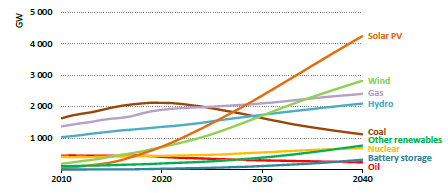
\includegraphics[width=10cm]{GlobalEnergy.PNG}
\caption[Evolution of total generation capacity under Sustainable Development Scenario by IEA]{Evolution of total generation capacity under Sustainable Development Scenario by IEA \cite{WEO}}
\label{Figure:global}
\end{figure}
\newline 
\noindent
In addition to the growing importance of small-scale renewables, a second trend in the electricity market that enhances the effect of utility death spiral is the gradual liberalization of the electricity market, especially in the European Union. The design of the market in its current state allows participants to join into the open market and set up some local DERs generation to fill up a local demand gap. In reality, however, this local DERs adoption is often performed by individuals with little information concerning the market because of the absence of active demand side management and access to real-time information. DERs adoption will, therefore, often be done by actors with limited or imperfect information about the market they are operating in. This imperfect DERs adoption and operation will often impose an additional burden on the utilities and grid operators, since the DERs will cause additional stresses on the grid, making it more challenging for the utility providers to maintain grid balance and stability \cite{EnergyMarket}. 
\newline \newline \noindent
One of the implications of these trends in investments in electricity generation assets is that many more actors will be involved in the investment decision making process, since the nameplate capacity of DERs is lower than that of large generation plants. Whereas historically one central decision maker would choose in what assets to invest, there is a gradual evolution towards a situation where, in theory, every household could make a decision about their means of electricity production and storage. These two opposing scenarios have their implications on the way investment decisions are made. A central decision maker will, most likely, be well informed about all options that can be invested in. In addition, he will likely make decision on a rational basis, since he has dedicated research teams to do so. A household, on the other hand, will be less informed and rational in its investment decisions related to electricity generation assets. In the context of the energy transition and reducing the consumption of fossil fuels of emission of GHG, reducing or transforming the energy consumption on a household level is an important step in the global emission reduction effort \cite{Totalenergy}. Of this total energy consumption, electricity consumption contributes significantly. A good understanding of the investment decisions in electricity related items on a residential level, therefore, is of major importance to be able to make the reduction in overall emissions as efficient as possible. So far, however, this potential has remained underdeveloped \cite{underdeveloped}. In this Thesis, therefore, these investment decisions will be further investigated with a particular focus on the effects  of the DERs adoption on the utility death spiral.
\newline \newline \noindent
The research that has been hitherto conducted in these areas has often had a large amount of assumptions about the actor's behavior that imply rationality, full information and an objective assessment of all facts available. To accurately model the behavior of households or individuals, however, these assumptions must be tweaked. As mentioned earlier, in the current liberalised electricity market, all actors can participate in the supply side of the electricity market, often lacking decent information on the demand, balance and pricing that prevails in the market \cite{EnergyMarket}. Rather than considering the objective value of a few different options to invest in, the crucial parameter in household decision making is the subjective value an actor will attribute to several decision options. These behavioral decision phenomena have been extensively researched in behavioral economic theories like expected utility theory, rank-dependent utility theory and prospect theory. These theories, especially prospect theory, are the basis for the analysis of decision making by individuals or households.  
\newline \newline \noindent
Although these behavioral finance theories are useful in increasing the understanding of decision making by households, the only subjective value (or utility) they consider is an economic one. The decision making of a household in DERs adoption, though, is one that has more motivations than a purely economic one. In the case of individual or household-level decisions, there are social, cultural, environmental and other circumstantial factors that need to be accounted for. In the scope of this Thesis, these additional effects will be represented as the social utility of an investment decision. This will be done through the peer influence, which will consider the influence actors can extert on each other in their decision making \cite{peer}. 
\subsection{Research question and contribution}
The general aim of this research is to determine what the effect is of different policies on DERs adoption and the utility death spiral. These policies include annual net volumetric tariff, annual offtake capacity tariff, net billing and battery subsidies. The main research question of this Thesis, therefore, will be:
\newline\newline
\textbf{Research question 1: What is the effect of annual net metering, annual offtake capacity tariff, net billing and battery subsidies on both households' DERs adoption under uncertainty and the utility death spiral?}
\newline\newline
Since prospect theory is used and interaction between households and the DSO is assumed, there are a some important variables in the system whose sensitivity to the model should be determined. An underlying question in this Thesis, therefore, is to what extent variables like risk aversion, peer influence and variable network charges, among other factors, will shape a household's DERs adoption. The effect of DERs adoption on the revenues of the utilities and distribution grid operators will also be examined. The implementation of prospect theory also gives rise to the thought of what the added value of this theory in this setting is. This objective motivated the following research sub-questions:
\newline\newline
\textbf{Research sub-question 1: What is the effect of risk aversion and network charges on both the DERs adoption on a household level and the utility death spiral?}
\newline \newline
\textbf{Research sub-question 2: What is the added value of using a cumulative prospect theory to model investment decision making, compared to expected utility theory?}
\newline \newline \noindent
These questions will be addressed within a defined scope: the spatial scope is a set of households interacting with each other and a DSO, while the time scope is the lifetime of the technology at hand (being about 20 years). The scope of this research is at the household level because the actors at this level of analysis have access to limited amounts of information and will often behave irrationally in their usage of this information. Thereby, they will take less rational investment decisions. In the development and analysis of this model, it is worth noting two matters. First of all, since this research focuses more on the qualitative insights rather than a quantitative forecast of a certain use case, insights into the different aspects of the model through extensive sensitivity analysis of all parameters are extremely important to gain a comprehensive understanding of the model dynamics. The parameters listed in Research Sub-question 1 (risk aversion, peer influence and network charges) are the most important ones, but other seemingly less influential parameters will also be tested. With these insights, the developed model can be compared with other models as to its results and parameter sensitivity, making Research Sub-question 1 complementary to Research Question 1. In addition, Research Sub-question 2 will address the novelty of CPT in the modeling framework by comparing the results those of the currently used decision making theory, being the EUT. By addressing this main research question and the two research sub-questions, sufficient insights into the model should be obtained to determine in which domains the model can be used for further research.
\subsection{Structure}
This Thesis consists of five chapters. In \textbf{Chapter 2}, the Literature Review, the in the relevant domains will be summarized. Here, the investments in DERs at the household level will be discussed. This will be done by initially focusing on the trends in DERs investments and a discussion of the different emerging DERs technologies, only to elaborate on the investment characteristics and drivers in the following section. Since it also is an important part of this research, the utility death spiral will be discussed separately. In \textbf{Chapter 3}, the Theory and Methods, the concepts and modeling considerations required to describe the DERs adoption will be discussed. This includes the discussion and implementation of the theories and methods that were resorted to in the model development. These include complex adaptive systems theory, prospect theory (and the concepts of behavioral economics like bounded rationality and sub-optimal decision making) and agent-based modeling. In \textbf{Chapter 4}, the Model Design, the theories and methods of Chapter 3 will be used to describe the model. First, the relevance of the chosen modeling techniques in the consumer-centric energy system of this Thesis will be discussed. Subsequently, the model will first be discussed conceptually, after which the model will be described in detail. In \textbf{Chapter 5}, the Results and Discussion, the data resulting from testing different policies in the model will be discussed. In the given framework of the model, this will be done by analyzing how the model results vary as a function of a few key parameters (Network charge, peer influence, loss aversion etc.). Note that the main goal is striving for qualitative insights here rather than quantitative predictions for a specific use case. In \textbf{Chapter 6}, after having discussed the results that the model provides, the key findings of this research as well as the model limitations will be discussed and placed in the broader perspective of the ongoing research.
\newline \newline \noindent
A graphical overview of the structure of this Thesis can be found in Figure \ref{Figure:struct}.
\newline 
\begin{figure}[h!]
\centering
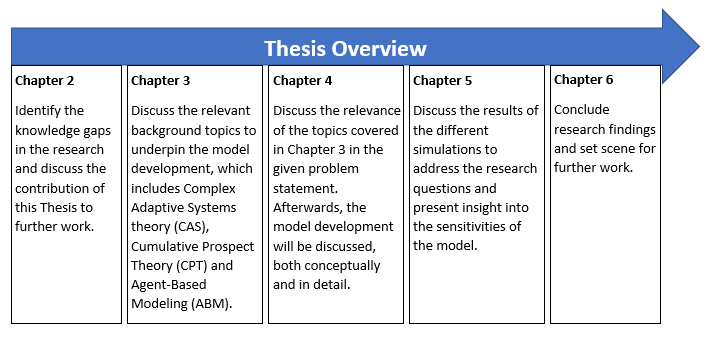
\includegraphics[width=\textwidth]{overview.PNG}
\caption[Overview Thesis]{Overview Thesis}
\label{Figure:struct}
\end{figure}
\newline 
\noindent
\chapter{Literature Review}
\section{{Introduction}}
This chapter will set the scene for the research performed in this Thesis by providing a thorough overview of the literature on investment decision making in the electricity sector, more specifically investments in DERs and the associated utility death spiral. In section \ref{Trends}, the nature and drivers of DERs investments will be discussed. First, the scene will be set by discussing the relevant technologies to this Thesis. These technologies are PV and residential battery storage. Subsequently, in section \ref{Investmentss}, the investment drivers and characteristics of DERs will be discussed, with a particular focus on PV. The possible negative effects of DERs, like grid stability issues, will also be discussed. One possible negative consequence of large scale DERs adoption, called the utility death spiral, will be discussed separately in section \ref{spiral}, since a great deal of attention will be spent on this trend in the electricity market throughout this Thesis. 
\section{Trends in DERs investment} \label{Trends}
\subsection{Introduction}
In this section, different trends in the DERs investment landscape will be discussed. When considering the broad definition of DERs, many technologies qualify as candidates. In this case, however, the discussion will be limited to three technologies. The first two are the most popular renewable energies/DERs: PV and wind power. The final one, battery storage, is much less popular than the two aforementioned ones, but is a very important one in the scope of this Thesis and will, therefore, be included in the discussion. Subsequently, some data will be presented concerning the investments and trends in the considered DERs technologies. There will also be a forward look into the required investments in the future to meet certain environmental/sustainability goals. 
\subsection{DERs technologies}
%To understand the emergence of DER, it is important to mention. Although the most important DER are solar PV and wind power, the latter will not be discussed since it is beyond the scope of this Thesis. 
 As mentioned earlier, the emergence of new electricity generation technologies is reshaping the generation and investment profile of the electricity market. A discussion of the different technologies that cause this transformation is important to understand the background of DERs. Covering all DERs technologies, however, is beyond the scope of this Thesis since many different energy technologies can identify as DERs. The two most prominent technologies in this perspective are solar energy (photovoltaics in particular). There are, of course, other renewable energy sources available, like geothermal, tidal and hydropower, but their potential is limited compared to solar and wind, so investments in these technologies will not be considered. A second technology that will be considered in this Thesis is battery storage, since the model in this dissertation will consider the adoption of PV-battery systems. The characteristics, emergence and evolution of these technologies will be discussed in the following paragraphs
\newline\newline \noindent
\textbf{Solar Power}
\newline \newline \noindent 
Solar power, and photovoltaics (PV) in particular, have become very popular in recent years. Despite there being many environmental and technology-related reasons for the adoption of PV, economics remain the main considerations for PV adoption. Initially, this was due to financial aid given by the government, since solar panels (the main technology used for residential applications and solar panel parks) were too expensive compared to other electricity technologies. Subsidies were one of the first financial aids given by governments, followed by additional incentive schemes like net metering and feed-on tariffs, to name a few. Recently, however, solar panels have gained popularity without the benefit of government subsidies. In Flanders, the Dutch-speaking part of Belgium, for instance, the sales of solar panels reached their highest level last year since 2012, when the government subsidies for the installation of solar panels got abolished \cite{Zonnepanelen}. This indicates that solar PV is getting economically attractive, which can only enhance their popularity in the future. As discussed in Chapter 1, the global PV capacity was 480GW in 2018 and is set to become the most popular generation technology by 2040. 
\newline \newline \noindent
As can be seen in Figure \ref{Figure:1}, the Levelised Cost of Electricity (LCOE) of solar PV has experienced a steep decline throughout the period 2012-2017. In all considered regions (China, India, Japan, United States and European Union) the LCOE decreased by more than 50\  over this period. Although already showing a historical decrease, the LCOE is likely to decrease further in the future, albeit not at the rate it has been in recent years. The data in Table \ref{table:1} shows how the different cost components of the cost are expected to evolve. Although the $O\&M$ cost is set to decrease over the next few decades, the main reduction in LCOE will be due to the decrease in capital cost. In the EU, for instance, the capital cost is expected to decrease from $1300\frac{\$}{kW}$ in 2017 to $760 \frac{\$}{kW}$, or 41\ .
\begin{figure}[h!]
\centering
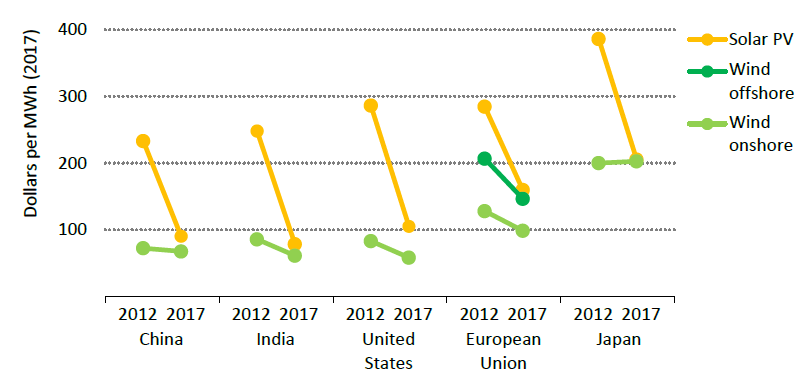
\includegraphics[width=10cm]{LCOE.PNG}
\caption[LCOE of Solar PV, Onshore wind and Offshore Wind]{LCOE of Solar PV, Onshore wind and Offshore Wind \cite{WEO}}
\label{Figure:1}
\end{figure}
\noindent
\newline 
\newline
To elaborate further on this projected price decrease, it is important to note that this capital cost evolution depends on how PV adoption will evolve over the next few decades. This evolution for different IEA scenarios can be seen in Figure \ref{Figure:adopt}.
\begin{figure}[h!]
\centering
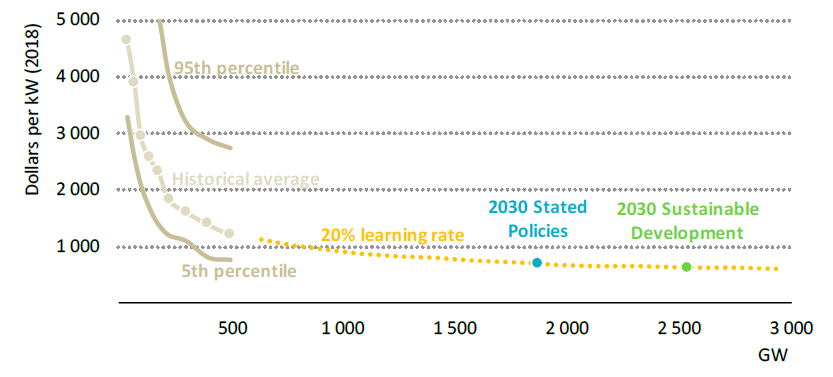
\includegraphics[width=10cm]{PVadoption.PNG}
\caption[Projection of PV capital cost]{Projection of PV capital cost \cite{WEO20}}
\label{Figure:adopt}
\end{figure}
\noindent
According to this Figure, the capital cost is set to decrease at a learning rate\footnote{The learning rate of a technology is the rate at which the cost will decrease if the cumulative installed capacity of the technology doubles} of 20\ . Depending on the adoption speed, therefore, the capital cost will decrease further. For both the Stated Policies and Sustainable Development, however, the capital cost is set to decrease significantly over the next few years. Since PV has no fuel costs, the capital cost decrease will have a major influence on the overall LCOE, which is also set to decrease further as time and adoption rates go by.  
 \newline \newline \noindent
% \textbf{Wind Power}
 %\newline \newline \noindent
 %Wind power, which is mainly exploited in the form of wind turbines, has become the most popular non-hydro renewable energy source in recent years. In 2018, 51.3GW of capacity was added, to bring the total wind power capacity to 591GW \cite{Wind18}. Like solar power, this adoption was initially fueled by government-backed incentives, followed by a decrease in price due to increased learning and scalability. As can be seen in Figure \ref{Figure:1}, the LCOE of onshore wind has seen a steady decrease (except in Japan) over the last few years. This LCOE is also expected to keep on decreasing, as can be seen in table \ref{table:1}.
%\begin{table}[h!]
%\begin{center}
 %\begin{tabular}{||c||c||c|c|c|c|c|c||} 
 %\hline
  %\multirow{\textbf{Region}} & \multirow{\textbf{Technology}} & \multicolumn{2}{c|}{\textbf{Capital} (\$/kW)} & \multicolumn{2}{c|}{\textbf{O\&M} (\$/MWh)} & \multicolumn{2}{c|}{\textbf{LCOE}     (\$/MWh)} \\  
   %\cline{3-8}
   %& & 2017 &2040 & 2017 & 2040 & 2017 & 2040\\
  %\hline 
%\multirow{USA}  & Nuclear & 5000 & 4500 & 30 & 30 & 105 & 100\\
 %&Coal & 2100 & 2100 & 30 & 35 & 75 & 75\\
 %&Gas CCGT & 1000 & 1000 & 30 & 40 & 50 & 65\\
%&Solar PV & 1560 & 860 & 10 & 5 & 105 & 50\\
 %&Wind onshore & 1620 & 1480 & 10 & 10 & 60 & 50\\
 %&Wind offshore & 4720 & 2960 & 40 & 25 & 180 & 105\\
%\hline
%\multirow{EU}  & Nuclear & 6600 & 4500 & 35 & 35 & 150 & 110\\
 %&Coal & 2000 & 2000 & 45 & 45 & 120 & 145\\
 %&Gas CCGT & 1000 & 1000 & 55 & 75 & 90 & 120\\
%&Solar PV & 1300 & 760 & 20 & 15 & 160 & 85\\
 %&Wind onshore & 1820 & 1700 & 20 & 15 & 100 & 90\\
 %&Wind offshore & 4260 & 2820 & 35 & 25 & 150 & 90\\
%\hline
%\multirow{China}  & Nuclear & 2320 & 2500 & 25 & 25 & 60 & 65\\
 %&Coal & 800 & 800 & 35 & 30 & 50 & 70\\
 %&Gas CCGT & 560 & 560 & 70 & 90 & 85 & 115\\
%&Solar PV & 1120 & 640 & 10 & 10 & 90 & 45\\
 %&Wind onshore & 1200 & 1180 & 15 & 15 & 70 & 65\\
 %&Wind offshore & 4120 & 2740 & 35 & 25 & 145 & 90\\
%\hline
%\multirow{India}  & Nuclear & 2800 & 2800 & 30 & 30 & 70 & 70\\
 %&Coal & 1200 & 1200 & 35 & 35 & 60 & 55\\
 %&Gas CCGT & 700 & 700 & 80 & 90 & 95 & 105\\
%&Solar PV & 1120 & 620 & 10 & 10 & 80 & 40\\
 %&Wind onshore & 1080 & 1040 & 10 & 10 & 60 & 50\\
 %&Wind offshore & 3320 & 2220 & 40 & 25 & 155 & 95\\
%\hline
%\end{tabular}
%\end{center}
%\caption[Overview of capital intensity of different technologies]{Overview of capital intensity of different technologies \cite{WEO}}
%\label{table:1}
%\end{table}
 %\newline 
% Despite the hype that exists around wind power, this technology has a few major issues. The first one is the fluctuations in the power output \cite{WindDisAd}. The second one, which is a result of the first one, is the sudden stresses wind power can cause on the grid stability \cite{WindStability}. When talking about wind power, however, one must make a distinction between onshore and offshore wind power, since both technologies do have some difference in costs, operation and regional popularity.
% \newline \newline \noindent
% Onshore wind has been deployed in most regions around the world. First developed in the 1980s, this technology gradually expanded through the 1990s to become a well-established technology. Over time, many countries started adopting wind power to make it achieve its state of popularity it enjoys now \cite{Onshoreoffshore}. Of the 51.3 GW that was installed in 2018, 46.8 GW was onshore (about 91.2\  of the overall installed capacity). The main advantages of onshore wind are its ease of installation, lower cost of installation and less maintenance difficulties. The disadvantages of the technology are its limited size potential, visual and auditive obstruction, and less constant wind patterns.
% \newline \newline \noindent
% Offshore wind is a smaller but very popular branch of wind power which is steadily increasing in capacity in Nothern Europe (note how data on offshore wind power is only available for the European Union in Figure \ref{Figure:1}). In 2018, only 8.8\  (or 4.5 GW) of all installed wind power capacity was offshore \cite{Onshoreoffshore}. Despite being more challenging to construct and maintain, the overall production and potential of offshore wind is higher than onshore and is so far underexploited.
% \newline \newline \noindent
% Due to its popularity, wind power has been severely decreasing in price over the last few years across all regions, as can be seen in Figure \ref{Figure:1}. This price is expected to decrease further in the future, as can be seen in table \ref{table:1}. In the EU, the capital cost for onshore wind power is projected to decrease from $1820\frac{\$}{kW}$ in 2017 to $1700\frac{\$}{kW}$ in 2040, a 6.6\  decrease, while offshore wind power is projected to decrease from $4260\frac{\$}{kW}$ in 2017 to $2820\frac{\$}{kW}$ in 2040, which is a decrease of 33.8\ 
% Fueled by this popularity, the amount of wind power capacity is expected to triple by 2040, as can be seen in Figure \ref{Figure:global}. Some even claim this technology has sufficient potential to meet the worlds entire electricity demand if well managed \cite{WindPotential}. Fueled by continuously decreasing costs (up to 40\  by 2050), the technology is often called a 'game-changer' in the electricity generation transition.
% %\newline \newline \newline \noindent
%\newline \newline \noindent
\textbf{Residential Batteries}
\newline \newline \noindent
The need for residential storage is becoming a major concern for the efficient implementation of DERs in a residential context because of the intermittent character of renewable energy technologies. Due to the mismatch between PV production and residential consumption patterns, storage is an important means to reduce the destabilizing grid injection of residential PV during peak production and low consumption. The amount of storage capacity on a global level, however, is very low compared to the overall production capacity, as can be seen in Figure \ref{Figure:storage}. The overall storage capacity was 2.2\  of the total generation capacity. Of this overall capacity, however, the vast majority of the storage infrastructure is pumped hydro storage (98.9\  of the overall storage capacity is in pumped hydro storage). Only a portion of the remaining storage capacity is battery storage. The overall battery storage capacity has historically, therefore, been very low. 
\newline
\begin{figure}[h!]
\centering
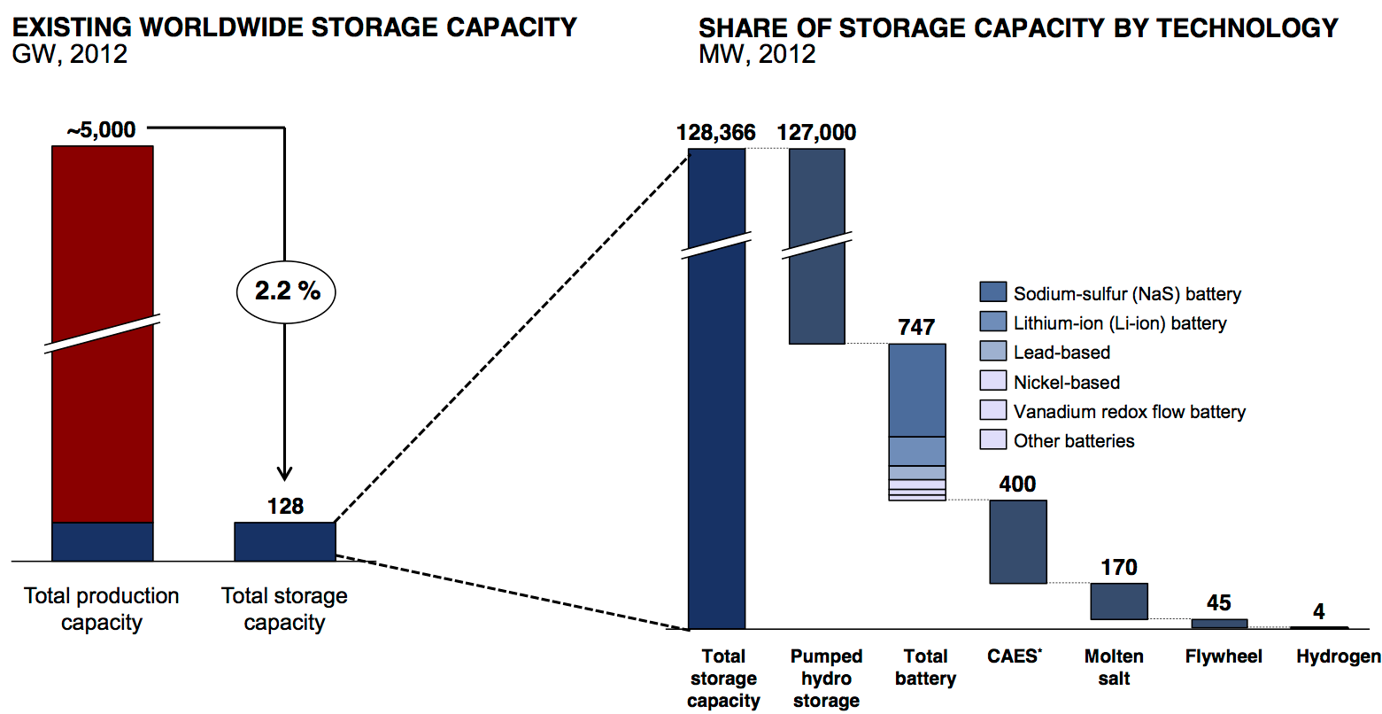
\includegraphics[width=10cm]{Storage.png}
\caption[Global storage capacity]{Global storage capacity \cite{Storage}}
\label{Figure:storage}
\end{figure}
\noindent
\newline
Even though the overall storage capacity in the world is very low and battery storage accounts for an even smaller portion of the overall storage capacity, storage capacity has been increasing rapidly, at a CAGR of 73\  between 2013 and 2018 \cite{Storage}. This large growth, however, will make the most recent values of the overall battery storage capacity (3.1 GW) still account for only a small portion of the global generation capacity. When comparing this value with the most recent data available for the global power generation capacity, which is a value of 7220 GW, it becomes clear the proportion between these two values is very unbalanced (the global generation capacity outnumber the battery storage capacity by a factor of 2329). 
\newline \newline \noindent
Since storage is often postulated as a major solution to the intermittent and unpredictable production patterns of wind and solar electricity generation, it may be interesting to consider what level of storage is required to allow for high renewables penetration in the grid. Solomon et al. tried to address this question by examining different cases of high renewables integration \cite{penetration}. In this research, the minimal amount of battery storage capacity required for a 90\  renewables penetration was determined to be the equivalent of the daily demand for electricity. To ensure minimal power loss, this storage capacity should be even higher. To ensure a reliable grid integration with large amounts of intermittent generation (i.e. large amount of solar and wind power, as is projected in Figure \ref{Figure:global}), the amount of storage will have to drastically increase over the next few decades. This increase require increased investments in residential battery systems, like Tesla Powerwall. Nevertheless, the emergence of electric vehicles (EV) can partially offset the need for investments in stationary storage capacity since EV batteries can also be used for residential storage purposes \cite{EV1,EV2}. 
\newline \newline \noindent
Despite being quite expensive nowadays, battery technology prices are expected to decrease rapidly over the next few years. Lithium-ion batteries, to take an example\footnote{In recent years, this technology has become the most promising battery technology, mainly due to its usage in Tesla and other electric automobiles}, have seen its levelised cost of storage (LCOS) decrease from \$1,160 in 2010 to \$176 in 2018, as can be seen in Figure \ref{Figure:bloom}.
\newline 
\begin{figure}[h!]
\centering
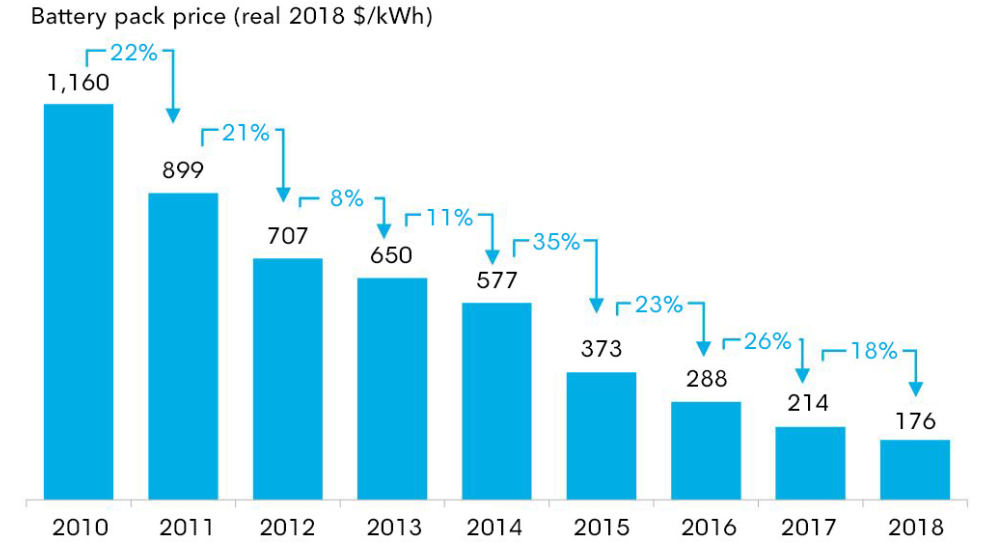
\includegraphics[width=10cm]{LCOS.PNG}
\caption[LCOS of Lithium-ion]{LCOS of Lithium-ion \cite{bloomberg}}
\label{Figure:bloom}
\end{figure}
\newline 
This LCOS is expected to decrease further to 94 $\frac{\$}{kWh}$ in 2024 and 62 $\frac{\$}{kWh}$ in 2030 \cite{bloomberg}. This projected decrease in price, combined with the increasing demand for batteries for grid integration purposes, will cause battery adoption to increase significantly over the next few decades, as can be seen in Figure \ref{Figure:global}.
\newline \newline \noindent
\textbf{Other}
\newline \newline \noindent
Although there are many more emerging technologies that can be implemented in a distributed context, these go beyond the scope of this Thesis. A quick enumeration of these technologies, however, will still be done. Wind power, both onshore and offshore, is the most prominent one. Another one is geothermal heat on a residential level, where ground heat is used for passive cooling and heating on a residential level. In this Thesis, electrical storage is considered, but thermal storage is also a form of DERs that is gaining popularity. Other forms of DERs include small hydro, biomass, biogas and small wind turbines.

%\subsection{DERs investment data}
%Having discussed which technologies are shaping the future electricity system, an overview of investments and capacity additions of these technologies will be discussed. According to the International Energy Agency, worldwide investments in electricity generation, networks and storage amounted \$750 billion in 2017 \cite{WEO}. Of the overall investment amount in electricity generation assets, two-thirds went to renewable assets. Figure \ref{Figure:RESINV} shows how these investments in different renewable energy technologies have evolved in the period 2013-2017.
%\begin{figure}[h!]
%\centering
%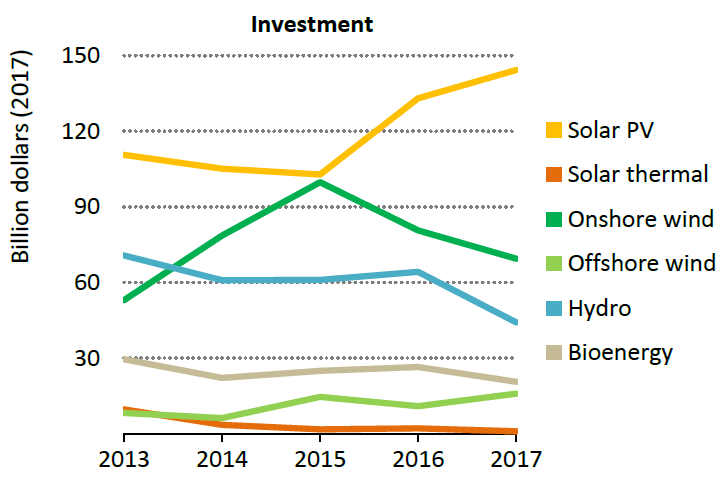
\includegraphics[width=8cm]{RESinvest.PNG}
%\caption[Global investments in renewable electricity investments]{Capacity for energy transition \cite{WEO}}
%\label{Figure:RESINV}
%\end{figure}
%\noindent
%\newline
%Judging by the evolution of the different curves in this Figure, solar PV is the most popular technology among investors in recent years. Surprisingly, investments in onshore wind decreased in the period '15-'17 after a period of growth in '13-'15. The investments in offshore wind, on the other hand, increased. The capacity additions that result from the investment data in Figure \ref{Figure:RESINV} can be found in Figure \ref{Figure:CAP}.
%\newline
%\begin{figure}[h!]
%\centering
%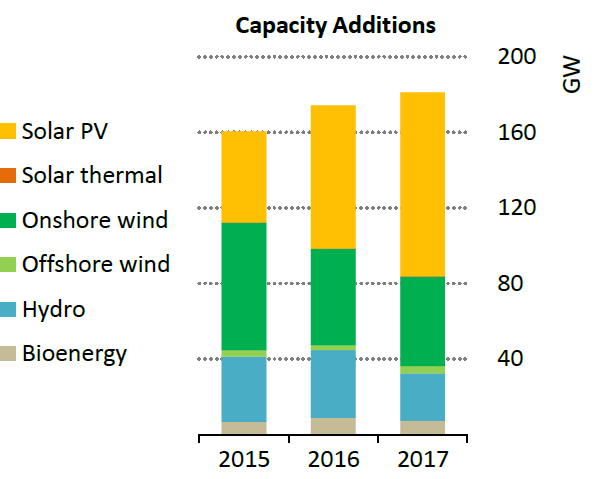
\includegraphics[width=8cm]{REScap.PNG}
%\caption[Global RES capacity additions]{Global RES capacity additions \cite{WEO}}
%\label{Figure:CAP}
%\end{figure}
%\noindent
%\newline 
%As is the case with the investment data, solar PV additions have been dominating the overall RES capacity additions in the period 2013-2017. When considering how these additions compare to the addition of fossil fuel electricity generation technologies like oil-fueled plants, coal-fired power plants, or CCGT, Figure \ref{Figure:comparions} shows that the amount of RES capacity added in 2017 surpasses the amount of conventional, fossil fuel capacity added in that period. This clearly shows how DERs, especially solar PV, are gaining popularity and will shape the future of the electricity market.
%\newline 
%\begin{figure}[h!]
%\centering
%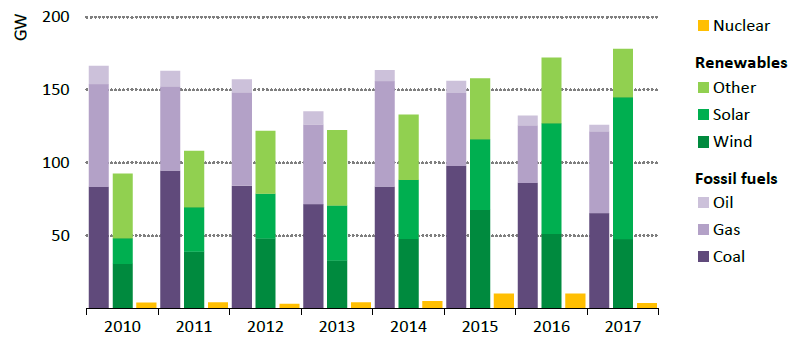
\includegraphics[width=10cm]{comparison.PNG}
%\caption[Global RES and fossil fuel capacity additions]{Global RES and fossil fuel capacity additions  \cite{WEO}}
%\label{Figure:comparions}
%\end{figure}
%\newline
%When looking into the future, the extent of the additional investments required in DERs and other renewables is also an interesting consideration. Since the call for a massive reduction of emissions is becomes more and more clear, there has been research into what the investment requirements are to meet a near-to-zero emission energy infrastructure over the next three decades, as was done by Jacobson et al. \cite{jacobson}. In this work, the cost of the New Green Deal to transition to a 100\  clean energy system was evaluated. This new infrastructure, consisting of wind, water and solar energy, increased efficiency and storage technology, is estimated to come at a cost of \$73 trillion if the objectives are to be met by 2050. The International Energy Agency estimates the cost of performing the New Policies Scenario and Sustainable Development Scenario at \$60 trillion and \$68 trillion, respectively, as can be seen in Figure  \ref{Figure:transition}. 
%\newline
%\begin{figure}[h!]
%\centering
%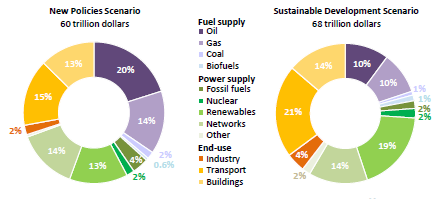
\includegraphics[width=\textwidth]{scenarioInvestment.PNG}
%\caption[Investment overview for IEA Scenarios]{Investment overview for IEA Scenarios \cite{WEO}}
%\label{Figure:transition}
%\end{figure}
%\noindent
%\newline
%Note how in both these scenarios, the investments in power supply are a substantial part of the total investments. For the New Policies Scenarios, the projected investments in renewable power supply technologies amount to 13\  of the total investment, or\$7.8 trillion, while for the Sustainable Development Scenario the portion for renewables is 19\ , or \$12.92 trillion. Although this is a sizeable investment amount for both scenarios, over time these goals must be met to ensure a sustainable energy infrastructure in the future.
\section{Investments in Distributed Energy Resources} \label{Investmentss}   
\subsection{Introduction}
In this section, the drivers, characteristics, and consequences of investments in DERs will be discussed. First of all, the characteristics of DERs investments will be discussed. This discussion will subsequently be narrowed to investments in PV and the resulting adoption patterns that arise from these investments. To conclude, a few points of attention in the investment in DERs and PVs, in particular, will be discussed.
% \subsection{DERs Investment Characteristics}
% When considering the installation of a PV-battery or another DERs, one must actually consider if this infrastructure expense is an investment altogether, since the costs a household must incur for a PV-battery installation is of the same magnitude as certain consumption goods\footnote{The investment in a PV-battery system, as will become clear in Chapter 3, is of the magnitude \$5,000 - \$10,000. Compared to certain household consumption appliances like electronics or transportation, this is a comparable cost}. An expense in a certain asset can be classified as an infrastructure investment if the following criteria are met \cite{infrastructure}:
% \begin{itemize}
%     \item \textbf{Asset exposure}: The infrastructure that is invested in consists of tangible assets.
%     \item \textbf{Stable, inflation-linked cash flows}: The infrastructure asset must generate a certain cash  flow that benefits the %investor throughout its operational lifetime.
%     \item \textbf{Long asset life:} The definition of a 'long lifetime' in this case refers to a value of  twenty years or longer. 
 %    \item \textbf{Uncorrelated to the equity markets, GDP and systemic risk}: The performance of the asset must  not be dependent on financial markets, as equities and fixed income do. This can either be for better or for  worse: the systemic risk of a financial collapse cannot directly influence the performance of the infrastructure asset.
     %\item \textbf{Direct investment can lead to low fees due to low maintenance costs}: The majority (or at least a large part) of the overall cost is in the capital investment into the asset.
 %\end{itemize}
 %When considering how an investment in a DERs like a PV-battery installation fits into these characteristics, there are a lot of similarities to be spotted. A PV-battery system is a tangible object. Since a PV-battery will cause the household to consume less electricity from the grid, the electricity bill for the household will be lower than it would have been if the household had not installed a PV-battery system. The cash flows the installation will generate are the savings caused in electricity cost due to lower gird offtake. Even though electricity prices tend to vary and are not inflation-linked, the cash flows that will be generated by this installation are going to be reasonably stable. 
% \newline \newline \noindent
 %The operational energy lifetime of a PV module is currently estimated about 20 to 25 years \cite{lifetime,lifetime2}. Given certain further innovations, this lifetime could increase to as much as 50 years \cite{lifetime3}. Throughout this lifetime, the cash flows will steadily be generated.
% Since the cash flow mainly depends on the electricity price, the effect of the financial markets and GDP is very limited in this cash flow generation. This electricity price is quite heavily regulated and will, therefore, not be completely exposed to the systemic risk of the equity and other financial markets. Finally, to comment on the last criterion, the maintenance and other operational costs of the PV-battery system are low, since there are no fuel costs.
 %\newline \newline 
% \noindent
 %The installation of a PV-battery system, therefore, clearly is an infrastructure investment. When considering what the actual characteristics of this DERs are, a few points must be commented upon. Olsina et al. listed several characteristics of power generation investments \cite{3}. Although this work concerns investments in power plants, these characteristics also apply to DERs investments. These include capital intensity, sunk cost, one-step investment, long-run uncertainties, long payback periods, investment irreversibility and investment postponement options.  
% \subsubsection{Capital intensity}
 %Although the investment in residential PV-battery systems is a limited financial commitment, this investment only accounts for a limited amount of production capacity. To get an idea of the overall capital requirements of DERs, table \ref{table:1} gives an overview of the cost components for different electricity generation technologies. Looking at the data in this table, it becomes clear that the capital cost of the renewable DERs still is higher than some conventional technologies. Solar PV still has higher capital requirements than gas CCGT in most regions, whereas offshore wind still is more expensive than coal-fired plants and gas CCGT. The second trend that can be noted, as has been discussed in section \ref{Trends}, is that the capital costs of renewable DERs like solar PV and wind power are set to decline significantly over the next few decades. 
% \newline \newline \noindent
 %Investing in DERs like solar PV and wind power, therefore, is a capital intensive process. To illustrate this, the data in table \ref{table:cost} shows the estimated capital requirement for different generation capacities. As can be seen, the total investment amount for an industrial-scale generation plant like Doel Power Station is very high, because of high capital cost and a high power plant capacity. The investment amount for a residential PV installation, on the other hand, is much lower because the capacity is much lower. 
 %\newline 
 %\begin{table}[h!]
 %\begin{center}
 % \begin{tabular}{||c|c|c|c||} 
 % \hline 
  %\textbf{Power plant} & \textbf{Technology} & \textbf{Capacity }(MW) & \textbf{Capital cost} (\$)\\
  %\hline
  %Doel power plant & Nuclear (PWR) & 2,923 & 19,291,800,000 \\
  %Ibbenbüren power plant & Coal-fired & 838 & 1,676,000,000\\
  %Amercoeur Power Unit & CCGT & 420 & 420,000,000\\ 
  %Vestas Wind Turbine & Onshore Wind & 4 & 7,644,00 0\\
 %PV installation & Solar PV & 0.004 & 5,200\ \
 % \hline
 %PV installation & Solar PV & 2,923 & 3,799,900,000\\
 % \hline
 % \end{tabular}
 % \end{center}
 % \caption[Nameplate capacity \& estimated capital cost of different]{Nameplate capacity \& estimated capital  cost of different %\cite{Vestas,Doel,Ibbenburen,Amercoeur}}
  %\label{table:cost}
 %\end{table}
 %\noindent
 %\newline 
 %When considering what the total investment in solar PV would be to obtain the same capacity as a large power generation station like Doel, it becomes clear that this amount is also considerable. Considering the load factor of PV panels is much lower than that of a power plant like a PWR or CCGT, the amount of capacity required for the same amount of energy produced will be much higher, thereby increasing the investment requirement even more. 
 %\subsubsection{Long-run uncertainties}
 %The combination of large investments, long lifetimes, and long payback periods pose a significant risk to the economic viability of DERs. A large number of possible risks exist, which can negatively influence the economics of the DERs. A few important ones are:
 %\begin{itemize}
 %    \item \textbf{Weather conditions}: Although not very important for fossil fuel power plants, this factor is very important for the emerging renewable technologies like wind and solar PV, since the performance of these technologies directly depends on the governing  weather conditions. Note that this uncertainty is predominantly short-run, since weather conditions can rapidly change, but also long-run to a certain extent due to changing weather patterns over the last few decades, as has been examined in Pakistan and the Himalayas \cite{Weather} and many more places around the world.
 %  \item \textbf{Future demand}: Depending on the future demand for electricity, the DER in construction or operation may not even be necessary at a certain point in the future. The fact that the generation capacity may potentially become obsolete in the future provides an additional level of uncertainty to the investment.
 %  \item \textbf{Long-term electricity prices}: The long term change in electricity prices can have a severe influence on the economics of any electricity generation asset. Since the economics of DERs depend on the potential savings they can realize, electricity prices are an important factor in assessing the economics of adopting a DER. If the electricity prices were to steadily increase over time, on-site production would become more attractive since the savings realized by the DER are going to increase, but if the electricity prices will decrease over time, the on-site production will become less attractive since the savings realized by the DER are going to decrease. 
 %\end{itemize}
 %Other parameters that need to be accounted for include:
 %\begin{itemize}
  % \item \textbf{Technological innovation}: The entry of more efficient technologies into the electricity generation landscape could easily substitute an existing technology, thereby making existing power plants or DERs unpopular. In the context of emerging small-scale technology, this is quite a big risk since the emergence of a technology could easily be hampered by another technology.
  % \item \textbf{Policy changes}: Since liberal electricity markets are relatively young, there is a continuous process of changing policies, which can influence the attractiveness of a certain generation technology. Especially for DERs, with government incentives like green certificates and Feed-in Tariffs (FiT) being regular topics of debate, these policy changes can pose a risk to the attractiveness of certain DERs. 
 %\end{itemize}
 %\subsubsection{Large sunk cost}
 %\noindent
 %Besides demanding large capital commitments, investments in DERs will also have what is called a sunk cost. This sunk cost, which is not only the case for electricity investments but any kind of dedicated infrastructure investment, is a cost that has already been incurred but that cannot be recovered. In the case of the electricity sector, a firm or another investor could incur a sunk cost if a certain power generation asset cannot be sold or transformed for another purpose without too much effort.
 %\newline \newline \noindent
 %In the current context of emerging technologies, conventional technologies with a long lead time and lifetime face an additional challenge. Throughout the lifetime of a certain electricity generation asset, technical progress comes in to play. The sudden emergence of a new energy technology could make certain DERs in use economically unattractive, forcing the investor to incur large costs \cite{Helm}.
 %\newline \newline \noindent
 %Although the absolute investment requirement for renewable energy technologies is lower, as was illustrated in table \ref{table:cost}, these technologies also have a very high sunk cost, proportionally even higher than is the case for conventional power plants. Renewable energy technologies like solar or wind do not have any fuel costs, contrary to conventional power generation. The majority of the costs in the technology, therefore, will be in the investment in the technology itself.
 %The sunk cost can, therefore, account for a very large proportion of the overall costs for DERs, posing a significant risk to the investor.
 %\subsubsection{One-step investment}
 %When installing a DER installation, a lot of functionalities must be fulfilled to make the unit operational. Therefore, a large amount of capital expenditures is required before the production capacity can become operational. Once this capacity is operational, the required capex required is merely maintenance capex and will, therefore, account for a limited amount of the overall capital requirements. 
% \subsubsection{Long payback period}
% The combination of a high overall cost and a large one-step investment for electricity generation assets will demand a high financial commitment by the investor, which often will be partially financed with debt. Over the duration of the operational lifetime, therefore, this debt will have to reimbursed. Considering the fact that the lifetime of a PV installation is about 20 years and 25 years for a wind turbine, the payback period for these assets can easily be years. There has been a some research in these matters \cite{Czec,CSP}. In \cite{Czec}, the payback period of a photovoltaic power plant was studied back in 2010, which came to 10-11 years, almost half the overall lifetime of the technology. In \cite{CSP}, the payback period of concentrated solar plant (CSP) was calculated, with results that go from 3.5 to 6 years, also a significant portion of the lifetime of a CSP plant. The overall payback period for DERs, therefore, is significant for different renewable energy technologies.
% \subsubsection{Investment irreversibility}
% The investment in generation capacity is considered a form of sunk cost, since a power plant can only serve the purpose it is designed for. If market conditions turn unfavorable and render the power plant unprofitable, there is little other purpose that the power plant infrastructure can serve. Even if it were to be sold, it would probably have to be done so at a loss. 
% There has been related work describing the irreversibility of investments in power generation \cite{irreversible}.
% \subsubsection{Investment postponement option}
% Since investing in a power plant or DER requires some financial commitment on behalf of the investor, it is very easy for the investing party to decide to postpone this decision. Especially in the context of investing in small-scale renewable technologies, where policies, tariffs and subsidies tend to change regularly, potential investors could easily choose to await new subsidies or tariffs before deciding to invest in DERs. In the case of DERs, there also is no immediate urgency for the technology to be installed, since electricity will remain available from the grid, which only adds to the possibility to postpone the investment. 
 \subsection{PV characteristics}
 \newline \newline \noindent 
 With the knowledge of the general investment characteristics of DERs, the scope can be narrowed to the technology that is under consideration in this Thesis, being solar PV. For the specific case of PV technology, there are a few specific investment characteristics that can be identified and can make it a preferred choice over solar powers greatest competitor, wind power. These can be grouped into three categories, as was identified by Ernst\&Young: operational, scalability and financial \cite{EY}.
 \subsubsection{Operational}
 There are a few potentials costs and benefits to investors because of technical characteristics of solar power. First of all, there will be less inherent production uncertainty, since solar irradiation forecast usually are more reliable than wind forecast. The increased reliability of the forecasts makes the future production of solar PV more certain, thereby making the future cash flows more certain, which makes the investment in solar PV more attractive compared to other intermittent DERs.
 \newline \newline \noindent
 In addition, the technology risk is lower compared to wind power due to less moving parts and few mechanical parts. Since residential PVs are installed on the roof of any residence, maintenance is very easy due to the accessibility of the installation. Compared to wind turbines (especially offshore), therefore, maintenance cost are much lower. Due to this major accessibility and fewer mechanical/moving parts, the lead time of a PV project, even a big one, is limited to months, compared to years for some large wind projects. 
 \subsubsection{Scalability}
 In addition to having interesting operational advantages, solar power has interesting scalability characteristics due its modularity. First of all, since solar panels can be fitted on any surface, flat or inclined at an angle, solar panels can be fitted anywhere. This makes it easy to install solar close to where the demand is, closer than any other renewable DER. Since the smallest unit size also is so small, the design of PV configurations is very modular and can range from kWs to MWs. Depending on the available space for installing solar PV modules, the number of modules can be adapted. Solar PV, therefore, is a very flexible technology in terms of installation and size, making it appeal to a wide range of investors, more than other DERs. 
 \subsubsection{Financial}
 As a final advantage, solar panels can also be a good investment for someone seeking returns on his or her investment. Ernst \& Young estimates that over the course of the next 35 years, the expected annual returns generated by investments in solar panels can vary anywhere between 6.6\  and 10.1\ , depending on how the efforts to combat climate change evolve \cite{mercer}. To put this into perspective, a US government bond will yield an annual return between 0.03\  and 1.30\ , depending on the maturity of the bond \cite{bonds}. The benchmark for the stock market, the S\&P 500, has had an average annual return of 9.8\  over the last 90 years \cite{stocks}. The returns of the solar panels, therefore, make a strong case for investments in because of good returns on investment.
 \subsection{Investment Drivers}
 As with many emerging trends, there are several drivers behind the emergence of small-scale renewables. These drivers cut across technical, economic, and environmental dimensions. Due to the increasing levels of pollution on a global level and the increasing awareness that this pollution might have dire consequences for the planet, there are strong environmental arguments for the rapid adoption of small-scale renewable DERs
 \newline \newline \noindent
 Since DERs will provide on-site production and storage of electricity, their adoption could have several technical advantages. First of all, since the DERs do not depend on the transmission or distribution grid for electricity production, remote communities can rely on these DERs to be self-sufficient in their electricity needs. In addition, grid operators will not need to extend their costly infrastructure to these remote areas to serve just a few customers. DERs, therefore, could avoid a great deal of expenses for the grid operators while making these remote communities self-sufficient. The case for the synergies that can be created by adoption DERs in remote areas has been made in numerous works for remote areas in Western Australia, Alaska and Canada \cite{remote1,remote2,remote3}. All this research strongly supports remote DERs adoption, provided that sufficient storage capacity is installed, to mitigate the risk of power shortages.
 \newline \newline \noindent
 In areas where there is a transmission and distribution infrastructure, DERs can help reinforcing the grid resilience by improving grid balancing. The importance of distributed resources for balancing purposes has been studied in other work \cite{balancing}. In this work, the authors were able to show that local storage devices are preferable compared to a central capacity. The authors in \cite{balancing2} also showed the usefulness of having local DERs assets for increased flexibility and balancing possibilities. In addition to these technical advantage associated with DERs, some other advantages have been identified \cite{technical}.  
 \newline \newline \noindent
 First of all, the DERs reduce the cost of energy, since the grid infrastructure doesn't have to be extended to all possible consumers if DERs can be adopted. Since more people can have access to electricity (and also heat and cooling when cogeneration is being used) by adopting DERs, the overall security of supply of the power system increases. Since production becomes more on-site and self-sufficient through DERs adoption, the reliability of the power system increases (since supply no longer depends on a central producer but many remote and local producers), which will make the consequences of a power outage on the grid less severe and costly. Since many of the DERs are renewable energy technologies, like solar PV, wind power and biomass, the adoption of DERs will go in parallel with a reduction of greenhouse gas emissions. Since more of the demand will be met by on-site production, there is also less need for constructing large generation units, relaxing the investment requirements for large utility providers. In the case of renewable DERs that don't require any fuel for operation, the fuel dependency, fuel cost risk and fuel supply will decrease for larger communities. Ancillary services can also be provided by DERs.  As a final point, DERs can increase the energy efficiency levels of the overall energy infrastructure. 
 \newline \newline \noindent
 Note how the three main pillars of sustainability, being security of supply, affordability and reduced pollution, all fit in the adoption of DERs. This is one of the reasons why this class of energy technologies is so promising for the future energy infrastructure.  
\subsection{Adoption of DERs on a household level}
Having discussed the characteristics and drivers of the investments in DERs, PV in particular, some empirical data on the adoption of DERs can be discussed. Since the focus in this Thesis is on the household level, it is important to determine    what the evolution of PV has been on a residential level and what the main drivers of this adoption are. There has been research into the diffusion of residential PV in different regions, such as Flanders \cite{FlandersAdoption} and Italy \cite{ItalyAdoption}. In addition there has been research into the evaluation of different policies related to PV technology and their effect on the evolution of PV adoption \cite{ABMPV}. 
\newline \newline \noindent
It may be interesting, at this point, to identify the main drivers of residential PV adoption, since this will provide insights for the model development in Chapter 3. In \cite{FlandersAdoption}, these drivers are identified. Since this work considers the drivers of Flanders, where the KU Leuven is located, an extensive discussion of these drivers is appropriate. The main drivers were identified to be: 
\begin{itemize}
    \item \textbf{Local subsidies}: These incentives, as there are green certificates and net metering, have had a significant impact on the adoption of PV technology in Flanders, especially when the cost of this technology was significantly higher in the recent past. Additionally, the more regional subsidies and incentives also seem to have benefited the evolution of the PV adoption rates.
    \item \textbf{Dispersion of income}: Through these subsidies, it was found that mostly rich households were able to benefit from these subsidies. The average income and economic status of the household adoption the PV, therefore, is also an important driver of PV adoption. 
    \item \textbf{Value of a house/household size}: With respect to the previous driver of PV adoption, it should be noted that an additional driver for PV adoption is the household size and house ownership. Since a larger family will, on average, consume more electricity, the incentive for PV adoption will be higher. On average, larger households will also have houses that are more conducive to the installation of PV technology, thereby increases adoption in this household category. If a certain households is the owner of a house, the decision power lies only with the occupant of the house, since he is the owner as well. This will make PV adoption more likely in this household category. If,on the other hand, the household is renting the house, the decision power lies with an external party, making the adoption of PV less likely.
    \item \textbf{Household characteristics}: A final aspect that will determine PV adoption is the 'characteristic' of the household, most importantly the age and size of the house. Overall, PV adoption is more likely in large or recently built houses. Since younger families will, on average, live in more recently built homes, this age category will have a larger percentage of PV adoption.  Despite this possibly being a result of changing mores between generations, the authors in \cite{FlandersAdoption} argue that this mainly is due to the fact that younger families will live in younger houses, not the actual age of the family.  
\end{itemize}
To elaborate on a few of these items, Palmer et al. showed that the economic profitability of the investment (through decreasing prices and subsidies) is the largest driver for adoption. In addition, the adoption will be the most stimulated by a gradual withdrawal of supportive measures, rather than abruptly withdrawing these \cite{ItalyAdoption}. As is the case in this Thesis, the authors consider different drivers than merely the economic ones, like the environmental and communication aspect in new technology adoption. The weight of these non-economic decision factors is lower than the economic weight. Their influence is also of limited duration. Over the longer term, the popularity of the PV technology will depend on the economic viability of this technology. De Villena et al. studied how different regulatory frameworks and incentive schemes by the government could influence the economic attractiveness of certain DERs \cite{Regulation}. To incentivize the DERs adoption, volumetric distribution rates rather than fixed ones should be implemented. The authors also determined net billing to be a better alternative than net metering to minimize the effects of the utility death spiral in the grid (see section \ref{spiral}). This work, however, assumes full rationality of the agents. Robinson and Rai use bounded rationality to determine factors influencing energy technology adoption \cite{spatiotemp,spatiotemp2}. An interesting finding in their work is the required incentives for PV adoption in lower-income. To have a significant impact on the adoption levels among low-income household, the rebates/incentives in PV cost must be substantial. Another interesting finding is in the time dependency of the rebate levels. If rebate levels are changed early in a program, when the amount of adopters is limited, the effect on the technology adoption is limited. If this rebate level is changed in a later stage of adoption, when the number of adopters is much larger, the effects will be more visible, since the social effect between adopters will cause the adoption to change. Zhao et al. argue that besides the household profile and the payback period of the PV, there are other factors at play \cite{ABMPV}. These mainly include the advertisement effect and the neighborhood effects. These two effects will account for the human perception of the product. In this Thesis, this will be represented as social utility (see Chapter 3\&4). From a technical point of view, Murakami combined the analysis of electric power flows from residential PV and social effects to determine how social policy and neighboring effects influence the diffusion of residential PV configurations \cite{flowanalysis}. The research points at that government intervention with regards to reverse current in the grid due to grid injection by peak PV production during periods of low demand, can have significant effects on the PV technology diffusion. By limiting the permitted reverse current, especially close to high-power distribution transformers, the diffusion is further enhanced. This will cause less variations in the voltage levels in the grid, reducing fluctuations and the need for batteries, which reduces to overall cost of DERs adoption. In areas located further from the distribution transformers, this reverse restriction must be relaxed since the overall system cost will increase due to higher requirements in battery capacity. The batteries are necessary to compensate for the lost possibility to inject power into the grid, causing the overall system cost to increase.
\newline \newline \noindent
When taking a step back from the adoption drivers and considering the adoption data itself, it becomes clear that PV is undergoing a rapid growth trend, as has been discussed in Chapter 1. The CAGR of the PV capacity (36.9 \  between 2010 and 2018) shows to what extent the global PV capacity has been growing. The future evolution of PV capacity can be found in Figure \ref{Figure:PVfut}. When focusing a bit more on the exact split between the different kinds of configurations installed, Figure \ref{Figure:split} shows that for the case of Italy, most of the installed PV installations in 2010-2011 had capacities between 1 and 20 kW, which is a size that can be implemented on a residential level.
\newline 
\begin{figure}[h!]
\centering
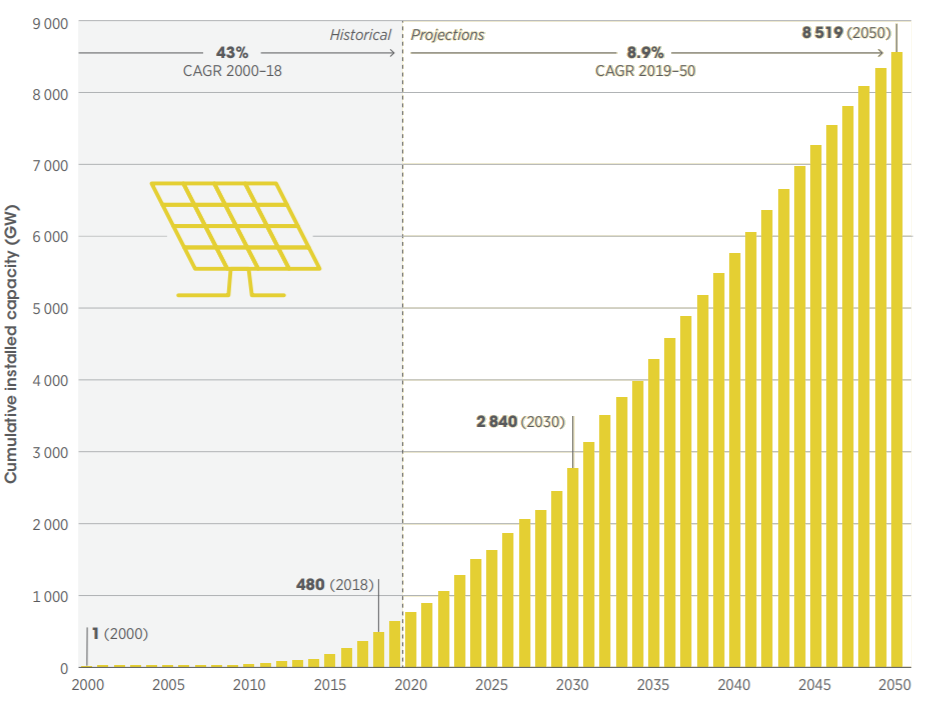
\includegraphics[width=6m]{PVfuture.png}
\caption[PV capacity evolution]{PV capacity evolution \cite{PVevolution}}
\label{Figure:PVfut}
\end{figure} 

\newline 
\begin{figure}[h!]
\centering
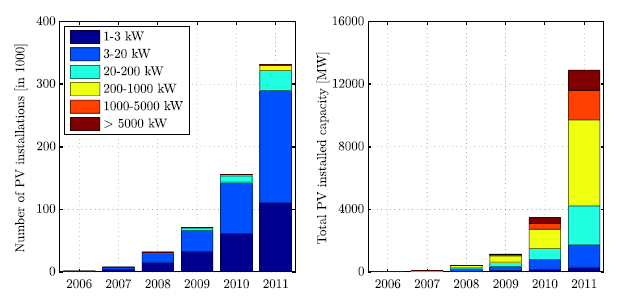
\includegraphics[width=10cm]{PVsplit.PNG}
\caption[PV configuration split]{PV configuration split \cite{ItalyAdoption}}
\label{Figure:split}
\end{figure}
\newline 
When looking at the overall capacity, however, it seems that the majority of the installations are in the range of 200 kW - 1MW. These installations, which may appear on large buildings or industrial estates, are also an important part of the overall PV adoption Figures. The adoption of PV on a residential level, therefore, is a consequence of various socio-economic factors. While social and other circumstantial factors play an important role in explaining adoption on a residential level, the economic consideration in the investment decision process remains the most important one.
 \subsection{Potential drawbacks}
 Over the course of the last few sections, the potential benefits and drivers for the adoption of small-scale DERs have been discussed. There are, however, also a few potential drawback or risks of this large scale DERs adoption. These include large area requirements, intermittency, grid requirements, material usage and, finally, the utility death spiral. Since the latter is an important phenomenon in the scope of this Thesis, it will be discussed separately in the next section. The other items, being very important to the overall DERs adoption discussion but less relevant in this dissertation, will be briefly discussed over the next few paragraphs.
 \newline \newline \noindent
 As has been discussed in the previous section, DERs technologies like PV and wind power are going to become increasingly popular (see Figure \ref{Figure:global}). These intermittent electricity generation sources add a level of uncertainty and complexity to the grid, since the supply and demand patterns of a renewable electricity production market will rarely align. As was discussed in section \ref{Trends}, there will be an increasing demand for storage capacity to cover this discrepancy between supply and demand patterns. In addition, the grid itself will need updates, to make its functioning more flexible and allow all DERs to be integrate into the functioning of the grid. The solution for this increased flexibility is not straightforward, since there still is debate on both sides of the argument whether the solution is a smart grid or super grid \cite{integration2} and how emerging technologies like EVs will be integrated into this grid \cite{integration1}. 
 \newline \newline \noindent
 In addition to imposing strict requirements on the entire grid, DERs will require a fair amount of land area to be able to meet the sustainability goals in the future. In a study by Cheng and Hammond, the energy density (in $\frac{GWh}{km^2}$) was determined for a few different energy generation technologies \cite{land}. A glossary of the data can be found in table \ref{table:land}
 \noindent 
 \begin{table}[h!]
 \begin{center}
  \begin{tabular}{||c|c||} 
  \hline 
  \textbf{Technology} & \textbf{Land density $(\frac{GWh}{km^2})$}\\
  \hline
  Nuclear (diffusion) & 3233 \\
  %uclear (centrifuge) & 3371\\
  Wind onshore & 872.4 \\
  Wind offshore & 22.64\\
  Solar PV (mc-Si) & 61.84\\
  Solar PV (pc-Si) & 48.86\\
  \hline
  \end{tabular}
  \end{center}
  \caption[Land density different energy generation technologies]{Land density different  energy generation technologies \cite{land}}
  \label{table:land}
 \end{table}
 \noindent
 Looking at the data in this table, it becomes clear how big a difference there is in the energy production per unit of land for different technologies. The renewables technologies like solar and wind require a much larger amount of land to produce the same amount of energy as a conventional generation plant, like a PWR. Over time, as solar PV and wind power will continue growing, the amount of land required to accomodate these DERs will also increase.
 \newline \newline \noindent
 Another issue that has been gaining attention in recent years is the recycling of the materials of the DERs at the end of their operational lifetimes. If the projections in Figure \ref{Figure:global} turn out to be accurate, the amount of waste from DERs will gradually keep increasing over time. At the moment, there still is no conclusive method for recycling end of lifetime DERs components. Turbine blades of wind turbines, for instance, are often dumped in landfills, rather than being recycled \cite{recyclig}. For PV, the management of all materials coming from end-of-life units is also becoming an increasingly frequent problem. So far, however, only the European Union has specific regulation of PV waste. The US, Japan and other nations treat PV waste as industrial waste. Since the recycling of PV waste could contribute significantly to the PV value chain, introducing specific measures on the recycling and treatment of PV waste is a necessity in the future as the amount end of life panels and waste will pile up \cite{recycling}. 
 \newline \newline \noindent
 A final issue with DERs and PV in particular is the utility death spiral. Since this is quite an important topic, this will be discussed separately in the next section. 
\section{Utility Death Spiral} \label{spiral}
\subsection{Introduction}
In section \ref{Investmentss}, the different consequences, both positive and negative, of the increasing levels of DERs adoption were discussed. An important one, called the utility death spiral, was not discussed since it deserves more attention in the scope of this Thesis. Since this utility death spiral is a serious challenge to the current business model of the utility providers, it will be discussed separately in this section. First, the phenomenon will be discussed and since there still is a strong debate among academics about the extent to which this utility death spiral could manifest itself, different positions in this debate will be presented. Subsequently, some possible solutions to the utility death spiral, if it were to become a problem, will be discussed. 
\subsection{Phenomenon description}
The concept of the utility death spiral emerged for the first time in the early 2010s, when the adoption trend of residential PV started to catch on. The first time this term was used in mainstream media, was in an article by the Wall Street Journal in 2013 \cite{wsj}. In this article, an analysis of the utility market was presented. Over the course of the article, the historically stable and indispensable nature of the utilities industry is questioned given the emerging trend of increasing PV adoption. The idea behind the utility death spiral is that due to the gradual adoption of PV, residential batteries and other DERs, consumers/prosumers will become increasingly self-sufficient in fulfilling their electricity demand. Consequently, these households will consume less electricity from the grid. Occasionally, however, the household will still require the services of the grid, in cases of extremely high demand or extremely low DER production (for exampled due to extremely unfavourable weather conditions for a limited period of time). The utility provider/grid operator will, therefore, still need to maintain its infrastructure for lower volumes consumed, which will force him raise his tariffs to offset the lost revenues due to the decreased consumption. This increase in prices will encourage more households to adopt DERs since the savings are greater, which will decrease the grid consumption again which, in its turn, which will force utility providers to raise his prices again and so forth. This reinforcing feedback loop is schematically represented in Figure \ref{Figure:spiral}:
\begin{figure}[h!]
\centering
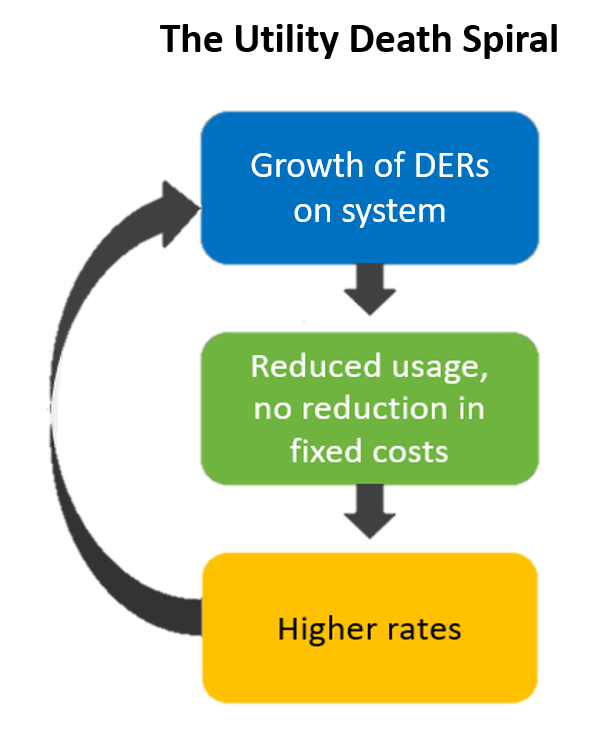
\includegraphics[width=4m]{UtilityDeathSpiral.png}
\caption[Representation of the utility death spiral]{Representation of the utility death spiral \cite{spiral}}
\label{Figure:spiral}
\end{figure}
There are different trends that have been causing the debate surrounding the utility death spiral, as was discussed by Graffy and Kihm \cite{spiralcauses}. Since the emergence of PV adoption is the main cause for the utility death spiral discussion, the reasons for this discussion are the same as the ones that caused PV to become a popular energy technology. As has been discussed in section \ref{Trends}, the main reasons for this are environmental (less GHG emission), technical (less central production, less risk for complete outages \& less stress on grid) and economic (subsidies \& decreasing prices PV technology).
\noindent
One of the reasons why this death spiral is happening, is due to the costs of the electricity transmission and distribution infrastructure being fixed, whereas the fees to the customer are often volumetric, i.e. they are a function of the end consumer's demand \cite{spiral2}. There has been research into the extent to which the utility death spiral has already been manifesting itself \cite{spiral3}. In this research, the effects of PV adoption on the revenues of the utility provider is limited since there is ample non-residential (commercial) demand which, combined with the declining residential demand, will cause the consequences for the TSO/DSO to be limited. Another finding from the research is that the transition to the large PV adoption state will be a smooth one rather than an abrupt one. Darghouth et al. studied how different electricity infrastructure rates influence the feedback on PV deployment \cite{fixedvar}. Since both fixed and time-varying rates will exist in the electricity market, different feedback loops will balance the equilibrium of this market. The fixed tariff will include a positive feedback
\newline \newline \noindent
Despite that there are some signals to confirm the utility death spiral is a consequence of PV adoption, there also voices who suggest that this is due to the traditional tarifing structure of the utilities \cite{spiral4}. Since DERs owners still rely on the distribution infrastructure, not only as consumer but also as producers, a redesign of the distribution tariffs will need to happen. This solution, along with others, will be discussed in the next subsection. A possible way to redesign the tariff structure, as has been proposed in the discussed literature, is by splitting up the fixed and variable costs the grid operator has to incurr and charge the end customer accordingly (based on the grid usage and electricity consumption). This way, DERs production and consumption can be rewarded more efficiently. 
\subsection{Possible solutions}
A possible way to redesign the tariff structure, and thereby mitigate the utility death spiral, as has been proposed in the discussed literature, is by splitting up the fixed and variable costs the grid operator has to incur and charge the end customer accordingly (based on the grid usage and electricity consumption). This way, DERs production and consumption can be rewarded more efficiently \cite{spiral4}. 
\newline \newline \noindent
There are three other ways utilities are exploring to mitigate the potential effects of the utility death spiral, according to an article by Forbes \cite{solutions}. The first one, which is in line with the aforementioned solution, is a transformation of the business model. In doing so, utility providers will focus on ways to exploit the interaction between connected devices on the grid. In doing so, the most valuable locations for DER can be located, allowing for utility providers to adapt their services and pricing in these location to be in a better competitive position, rather than having a uniform electricity charge over the entire grid. In addition, increases in energy efficiency and the use of smart grid are to be compensated by the DERs prosumers. A second avenue that is being considered involves the emergence of EVs. This trend will increase electrification and, therefore, the amount of electricity and ancillary services required on the grid. Utility providers could capitalize on this new trend by offering charging services to the owners of these EVs, either by renting the infrastructure or renting subscriptions to intelligent charging platforms. A final way to combat the utility death spiral is modernizing the grid. To make this costly investment worthwhile for the utility providers, however, utility providers should focus on reducing pollution levels, reducing the average costs of the grid (by increasing the efficiency), increasing customer interaction and improving the grid reliability/resilience. In doing so, the intrinsic value of the grid can be enhanced, creating new opportunities for the utility provider.
\newline \newline \noindent
Although the emergence of DERs, PV in particular, is threatening the current state of affairs for utility providers, there are ample opportunities for these organisations to transform their business model and be prepared for the future. 
\section{Contribution to literature}
Whereas in previous work the adoption of DERs was studied using economically rational theories, like utility maximization or NPV, this Thesis attempts to capture the human character traits in investment decision making. Using cumulative prospect theory (CPT), the subjective perception of the economic utility is used as decision variable, rather than the NPV itself. By incorporating this subjective value, the behavioral traits of individuals, like loss aversion and the reference point of the decision maker will be accounted for. 
\newline \newline \noindent
In addition, this Thesis is one of the only works to study the relationship between DERs adoption on a residential level and the DSO revenues using an ABM. The work that has been done in this domain so far, however, assumed rational behavior by agents \cite{Regulation}. In this work, the adoption of DERs and evolution of network charges are evaluated for different energy-related policies. In doing so, however, the authors assume rational behavior by the electricity consumers. Behavioral traits like risk aversion are not considered in this work. The second major contribution of this Thesis, therefore, is the incorporation of behavioral decision making character traits in the interaction between DER adoption and network charges using
an agent-based modeling framework.
\chapter{Theory and Methods}
\section{{Introduction}}\label{intro}
\newline \newline \noindent
In this chapter, the theories and methods used in this Thesis will be the main point of focus. The problem under consideration is the adoption of DERs and the utility death spiral for different policies. In this system, there will be many complex processes going on in the system, like emergence, adaptation, prediction, and state-based responses because of the interactions between different households and the DSO. Therefore, the system under consideration, it will be treated as a complex adaptive system (CAS). Since this type of system requires an appropriate modeling technique to account for all the complexities and details embedded within its structure, agent-based modeling (ABM) is an appropriate modeling technique to do so. Within the ABM, a decision making theory will be required to account for the decision-making patterns of the households in the investment process. Cumulative prospect theory will be implemented to incorporate human behavior in the decision-making process.
\newline \newline \noindent
In the following sections of this chapter, the different theories and methods are to be discussed. First, in section \ref{CAS}, the properties of CAS will be the main point of focus. Subsequently, in section \ref{Prospect}, the decision making theories relevant to this Thesis will be discussed. Since the selected decision making theory (cumulative prospect theory) belongs to behavioral economics, this broader topic of science will be the first point of discussion before elaborating on the specific characteristics and equations related to both prospect theory (PT) and cumulative prospect theory (CPT). In this discussion, a few alternatives to the CPT will also be highlighted, like the expected utility theory (EUT) and the rank-dependent utility theory. These different theories will also be compared to the CPT. In section \ref{Modeling}, the different modeling techniques that can be used to address the problem under consideration will be covered. These techniques include optimization modeling, equilibrium modeling and agent-based modeling (ABM). Each of these modeling techniques has its specific properties, advantages, and drawbacks, which will be discussed and synthesized in this section. In section \ref{approach}, research approach will be elaborated upon in detail in Chapter 4.
\section{Complex Adaptive Systems} \label{CAS}
The notion of what a complex adaptive system (CAS) entails is important in the selection of an appropriate modeling technique. The literature surrounding CAS, however, fails to give a formal definition or overview of what a CAS exactly is. Intuitively, however, the different characteristics of a CAS can be explained. According to \cite{ABM}, an adaptive system is one that, over time, will improve its relation to the environment. This can be any kind of environment: a physical, biological, social, technical or cultural one, just to name a few. Adaptations are not the same as change in response to a stimulus, since a change can be for better or for worse, whereas an adaptation always is for the better. These stimuli are from the environment itself and must also appear in some patterns in the system, either on a constant or a regular basis. Note that an adaptation is not the same as an evolution, since evolution is the aggregate effect (or algorithm) of all adaptations that produce all these improvements, as was examined by Charles Darwin in his "Origin of Species"\cite{Darwin}. Based on the stimuli that the system/environment will produce, therefore, agents in a CAS will gradually adapt their behavior to increase their synergies with the situation presented by the environment. This behavior is often referred to as self-organization. When a system develops over time, through emergent behavior, patterns and structures in the system will arise. These patterns and structures are not predefined in the model, but are a consequence of actions performed by the actors in the system. Self-organization is the result of these adaptive responses of the actors, which will gradually shape the system \cite{ABM}. 
\newline \newline \noindent
A complex system is, to put it bluntly, the opposite of a simple system. This simplicity can be either structural or functional. When simulating systems, however complex the assumptions and models are, there will always be some simplifications or limitations imposed on the system. In ABM, however, it is possible to capture these complexities to a decent level, allowing for the modeling of CAS. 
\newline \newline \noindent
Railsback identified several key characteristics of CAS for modeling the complex dynamic behavior of agents in a system \cite{6CAS}. These will be discussed over the next few points:
\begin{itemize}
    \item \textbf{Emergence}: One of the key elements of CAS is the emergence of system-level properties. Although the emergent behavior of the properties will occur on a system level, it is a consequence of the character traits of agents and individuals. If the emergence of properties follows from simple decision rules, it is possible to predict how different properties will emerge from different sets of decision rules. It is also a good guarantee that the model is general and can be applied to untested situations. The approach to system modeling, in this case, is very different compared to optimization and equilibrium modeling: rather than describing the CAS from a system level, which can require a large number of equations for advanced models, the system is described from an agent/individual level. For more complex models, this often allows for a more straightforward definition of the rules. The emergent response of agents cannot be confused with imposed response of agents. The latter forces agents to make certain decisions or perform certain actions in a specific situation. These imposed responses are often the result of what has been observed in real-world experiments. The validity of the imposed responses is, therefore, limited to the situations that have been observed in the field. For a generally valid model, therefore, the responses must be extended beyond the empirical situations available. Ideally, the model should be designed in a mechanistic rather than an empirical manner. The decision should also be formalized in a mechanistic way (i.e., the agent should make decisions or perform actions based on a minimal/maximal value of a certain parameter, surpassing a certain threshold value, etc.). In doing so, the empirical limitations of a model are removed. If the emergent response of a mechanistic model resembles the imposed response from the empirical findings, it is safe to assume that this emergent behavior is generally applicable to different situations. Therefore, the important traits of the agents are necessary knowledge to design a model.
    \item \textbf{Adaptation}: Together with emergence, adaptation is one of the core elements of CAS. As has been discussed in previous paragraphs, adaptation refers to the ability of agents to improve their fitness in their environment through behavioral changes. Depending on the complexity of the model, a system can show elementary or very advanced adaptive behavior. Although adaptation stems from biological evolution, which is an adaptive process that took many centuries, this behavior in CAS can occur in different spatial and temporal scales. As a function of these spatial and temporal scales, the relevant characteristics that must be adaptive can be identified: short-term adaptations must be a function of a relevant short-term event (like the adaptation of animals becoming more aggressive when they suddenly feel threatened) while long-term adaptations should be a function of the relevant long-term events (to stay with the animal example, the physiology of animals will adapt as the weather patterns in their environment gradually evolve).
    \item \textbf{Fitness and strategy}: The definition of fitness in the context of CAS must be clearly defined in the scope of the problem at hand. Fitness in a model is the state agents are seeking to obtain by optimizing their synergies with the environment. This seeking process will happen through a series of adaptive actions. The concept of fitness is important to define rules that will allow the agents to adapt their behavior. If fitness for the different agents is not defined, the adaptive actions cannot be clearly defined either. This fitness strategy can also be a function of the state of the agents and a function of time.
    \item \textbf{State-based responses}: Agents in the CAS will, since they will have adaptive character traits, respond to certain stimuli that the environment exposes them to. This response, however, is not a static response, but rather a dynamic response depending on the state or situation the agents finds himself in. Animals living in ecosystem, for instance, will hunt and move about depending on their fitness. In the case of investment decision making, people with large savings and capital reserves will be more likely to invest in new, uncertain technologies, whereas people with limited savings and capital reserves will be less prone to invest in such technologies.
    \item \textbf{Prediction}: Since the agents in a CAS show intelligent behavior, these agents will be able to predict or anticipate the occurrence and outcome of certain events. This anticipation and prediction is a result of a learning process from past experience throughout the evolution of the system. This predictive ability appears in the most simple CAS (bacterial models) as well as very advanced CAS (like population behavior models). Holland identified two different kinds of prediction: tacit and overt \cite{CAS}. Tacit prediction happens when actions are performed based on assumptions that are implicitly present in the model since they are considered commonly accepted knowledge (for example, underlying physical models in a system). Overt predictions happen on a more explicit basis since the assumption are explicit in the model and action will be taken accordingly. Decisions will be made by forecasting different alternatives and considering the consequences of these alternatives, only to choose the most promising alternative. Being able to distinguish the different alternatives and computing their possible outcomes is key in understanding the adaptive behavior of agents. 
    \item \textbf{Computer simulations}: For the vast majority of all cases, the simulation of agent behavior in CAS relies on computer simulations. Since the development of a CAS and its implementation in computer code almost always goes hand in hand, the formulation and implementation of CAS models must be considered jointly. In this perspective, an important part of the relation between the conceptual model and computer implementation is the user interface of the model. To understand a CAS and its adaptive/emergent traits, studying the input-output evolution of a model is very important, so the way in which a model will provide output to the user is very important. Although the representation of output variables increases the computational requirements of a model, it is a vital part of a computer program to understand and improve its functioning. If the output of a model is simply taken for granted and the model itself is treated like a black box, a recipe for disaster from a model validation point of view is presenting itself. In addition to having a good user interface, the model must be well documented in detail, since a small attribute of a model can easily render it erroneous. By fully documenting a model, it becomes easy to decompose and reproduce by other researchers. The ODD protocol can serve as a good framework to perform this model description. Finally, there must be sufficient quality control of the computer code and results that the model produces to ensure the validity of the model.
\end{itemize}
% justify the selection of ABM as a modelling technique
A visualisation of a CAS can be found in Figure \ref{Figure:CASS}. Here, the emergent behavior of self-organising sets of agents can be seen. The feedback loops causing the adaptive behavior between the environment and agents are also represented in the Figure.
\newline 
\begin{figure}[h!]
\centering
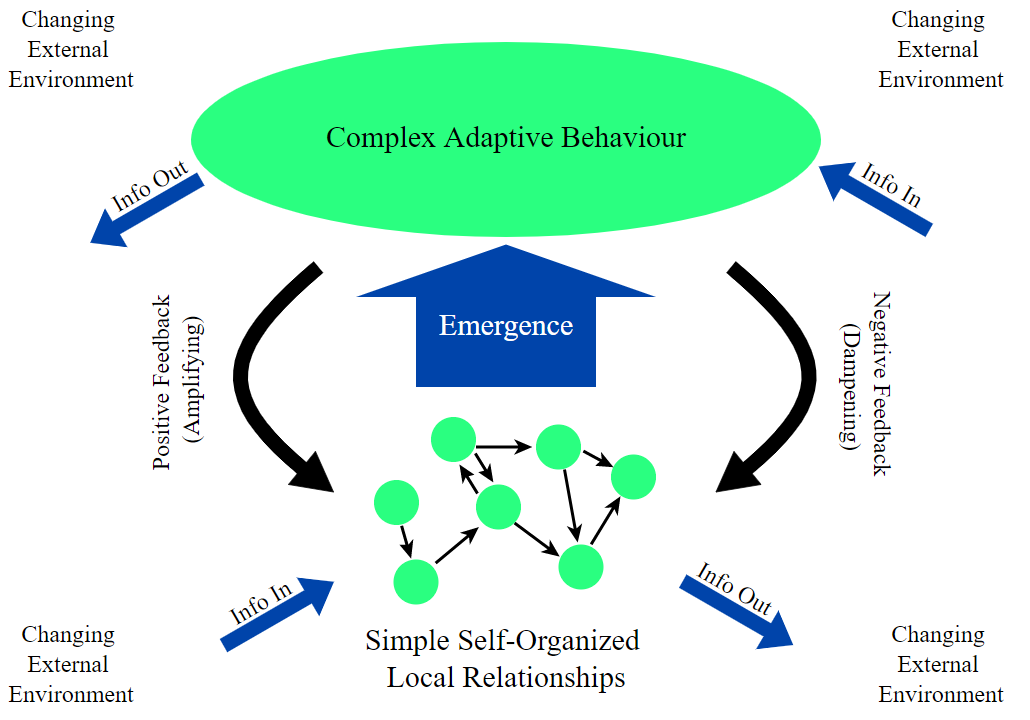
\includegraphics[width=10cm]{Complex_adaptive_system.png}
\caption[Conceptual example CAS]{Conceptual example CAS \cite{CAsexample}}
\label{Figure:CASS}
\end{figure}
\newline \noindent
Since these system characteristics imply a great deal of dynamics, like emergence and adaptive behavior, an appropriate modeling technique will be required to simulate these dynamics. As will be discussed in section \ref{Modeling}, agent-based modeling is the preferred technique over other techniques like optimization and equilibrium modeling.
 
\section{{Decision-making theories}} \label{Prospect}
\subsection{\large{Introduction}} 
Since the model in this Thesis deals with the simulation of decision making on a household level, an appropriate decision making theory must be selected to account for sub-optimal, irrational decision making traits. As will become clear over the course of this section, behavioral finance or economics are a branch of science that can help account for sub-optimal decision making on a household/individuals level. From the different theories in behavioral finance, cumulative prospect theory (CPT) will emerge as the preferred candidate for the simulation of decision making. 
\newline
\newline
Over the course of this section, the scene will first be set by broadly discussing behavioural finance and economics. Subsequently, the specifics of prospect theory will be discussed. In doing so, a brief history and a summary of the theory will be the main focus. Finally, prospect theory will be compared to other theories of choices under risk that have been developed over the last few decades in parallel with it. 
\subsection{\large{Behavioral economics}}
As the name suggests, behavioral economics deals with the economic implications of human behavior. In doing so, this starts from observations of actual human behavior, which behavioral economists attempt to formalize into a theory. Empirical data in this field will, therefore, constantly challenge a certain theory. Many theories in behavioral economics will subsequently only be as good as the experiments it describes. This makes it challenging for the theories to be operational, which is still is one of the major challenges in this branch of science. Although having been in development for many decades, behavioral economics has been gaining lots of popularity in recent years through recognition of the highest academic level for renowned scientists like Daniel Kahneman \& Vernon L. Smith in 2002 \cite{NobelKahne}, Eugene F. Fama, Lars Peter Hansen \& Robert J. Shiller in 2013 \cite{Nobelshiller} and Richard H. Thaler in 2017 \cite{Nobelthaler}. This recognition has strengthened the case for behavioral finance and economics, which strongly opposed itself to the classical economics theories of rational choices.
\newline \newline \noindent
In classical economic theory, which can be traced back to the principles first postulated by Adam Smith, many ideal assumptions prevail about decision making in economics \cite{adamsmith}. In a world existing under these assumptions, people make decisions based on fully informed calculations whose results they interpret rationally. These choices will also align with the best self-interest of the decision-making agent. This agent will often be referred to as the "homo economics", since the agent is assumed to be an economically rational human being, putting economic considerations in decision making before any other consideration. This approach to economic thinking was later incorporated in the theory that is often referred to as rational choice theory. This rational choice theory (RCT hereafter) serves as an umbrella term for theories in neoclassical economics, where the outcomes of certain actions can in some way be construed as rational \cite{RCT}. This "ensemble" of theories, often referred to as neoclassical economics, relies on three major assumptions:
\begin{itemize}
  \item Individuals have selfish preferences
  \item Individuals maximize their utility
  \item Individuals act independently based on full information
\end{itemize}
\noindent
The most "simple" version of neoclassical economics/RCT assumes that all individuals are fully informed about all decisions alternatives, the probabilities of their outcomes, their consequences and assumes no cognitive limitations for the agent in the processing of all this information. These assumptions are very strict and demanding and can, therefore, hardly be implemented for real-life experiments. Herbert Simon, therefore, introduced the concepts of bounded rationality in 1957 \cite{boundedrat}. This concept relaxes the assumptions of full rationality. Under bounded rationality, the agent/decision maker recognizes that gathering information is an energy and time demanding process, thereby limiting the amount of information that will be gathered and processed for decisions making. Whereas full rationality is the process of "maximizing" someone's situation, bounded rationality is the process of 'satisficing' a certain situation. 
\newline \newline \noindent
In its attempts to reshape economics as a natural science through rationality assumptions and terms such as the "homo economicus", the first economic theories on decision making imposed many ideal assumptions on the behavior of economic agents, creating a very artificial representation of certain models. Through his theory of bounded rationality, Herbert Simon put a limit to these assumptions by saying that rationality is constrained due to limited time to process all information available and limited tractability of the decision problem at hand. This already is the first step in the direction that humans or other decision makers will inevitably make suboptimal choices, away from the economically rational theory developed by neoclassical economists. By the end of the 1960s, as cognitive psychology became a more established and commonly accepted branch of psychology \cite{cognitive}, Kahneman and Tversky used this new development in science to lay the conceptual foundations of prospect theory, which will be discussed in the next section.
\subsection{\large{Prospect theory}} \label{ProspectTheory}
As discussed in the previous subsection, prospect theory (PT) is the result of many different stages in the transition from rational, neoclassical economics assuming that the "homo economicus" will always make economically optimal decisions, to the rationally bounded, cognitive agent that will make sub-optimal decisions that are satisfying, rather than optimal, to him. In this section, the different aspects of prospect theory will be highlighted and discussed. The development of prospect theory arose through lab experiments obtained by Kahneman and Tversky that diverged from the decision making theory that was widely accepted at the time, being the Expected utility theory (EUT). The authors, therefore, postulated a different version of decision making, which will be the main point of attention over the course of the next few paragraphs.
\newline \newline \noindent
When choosing among uncertain scenarios, an agent is choosing from a set of prospects or gambles \cite{prospect1}. A prospect is nothing more than an overview of different outcomes a certain asset evolution have, while taking into account the probability of all these different outcomes. Mathematically, this prospect can be represented as:
 \begin{equation}
     (x_1,p_1; x_2,p_2;...;x_n,p_n)
 \end{equation}
 Where $p_1$ is the likelihood that this contract of outcomes will yield the result $x_1$, $p_2$ the likelihood that the contract of outcomes will yield the result $x_2$, etc.. Note that that this set of probabilities is subject to the constraint:
 \begin{equation}
     p_1 + p_2 + ... + p_n = 1 
 \end{equation}
The assumptions EUT makes around these prospects (see section \ref{EUT}) had already been severely challenged by previous work. This can be divided into a few different parts. First of all, there was significant criticism in what is referred to as the \textit{certainty effect}. If this effect is manifesting itself, people overweight outcomes that are considered certain, relative to outcomes which are perceived as probable. A good case for this certainty effect is given in \cite{Allais}. What also arose from these test is that in a case where winning is possible but not probable (i.e. there are gains to be made but the likelihood of receiving them is small), most people choose the prospect that offer the larger gain. A second aspect where EUT failed, according to Kahneman and Tversky, is the incorporation of negative prospects. This effect, referred to as the \textit{reflection effect} by the authors of PT \cite{prospect1}, states that the preference between positive and negative prospects are the mirror image of each other. This brings with itself an important factor of PT, more specifically that risk aversion in the positive domain (i.e. when facing gains) is accompagnied by risk seeking in the negative domain (i.e. when facing losses). Parts of this theory had already been suggested by previous research, only to be reconfirmed by Kahneman and Tversky \cite{Marko} \cite{Williams}. Besides the two aforementioned criticisms, which are the main criticism PT had on EUT, there are many more mentioned in \cite{prospect1}, but a discussion of all these points are out of the scope of this research. It is worth noting that over the course of their academic career, Kahneman and Tversky provided an initial prospect value theory in \cite{prospect1} in 1979 and provided an update in 1992, called the cumulative prospect theory (CPT) \cite{prospect2}. Over the course of the 1980s, prospect theory came under increasing criticism by other theories, like the rank dependent theory (see section \ref{EUT}). In the classical theory, the utility of an uncertain prospect is the sum of the utilities of the outcomes, each weighted by its probabilities \cite{prospect1}. The new CPT, however, provides a few updates. Based on the finding of the rank-dependent utility theory, the probability function now is of the cumulative kind. Since CPT is the updated version of the initial PT, this is the version of the theory that will be used in this Thesis. Nevertheless, a quick overview of the original theory and its subsequent improvement will be given in the next few paragraphs
\newline \newline \noindent
The original PT divided the decision making process into two different stages: the editing phase and evaluation phase. This was done to avoid any violation of first-order stochastic dominance in the results. In the editing phase, all the options are laid out and reformulated to simplify the evaluation or organisation of the decision making. Different outcomes will be classified as either gains or losses compared to a certain reference point, which usually is the current asset position of the decision maker\footnote{A generally accepted definition of this reference point hasn't been formulated yet, which is one of the main reasons why PT is not operationalizable}. All prospects will also be simplified and segregated into riskless and risky prospects. This editing will be based on heuristics, which means that the decisions will be motivated by past experiences of the decision making agent. 
\newline \newline \noindent
Following the editing phase, the evaluation phase will kick off and the decision maker will value each of the prospects and choose the one with the highest value. This selection will be done according to the computation of the value $V(x)$:
\begin{equation}
    V(x) = \sum_{i=1}^{n} \pi(p_i)*v(x_i)
\end{equation}
\noindent
With $\pi(p_i)$ the decision weight and $v(x_i)$ the subjective value of the outcome to the agent. Note that at the time of the first publication of PT, there was no formal definition of how to compute these components. Together with the criticism that came once published, particularly from Quiggin's rank-dependent utility theory (see section \ref{EUT}), all these items were updated and formalised in the CPT \cite{prospect2}.
\newline \newline \noindent
The value function $v(x)$ in CPT can be described using the following set of functions:
\[   \left\{
\begin{array}{ll}
      x^\alpha & x \geq 0 \\
       -\lambda(-x)^\beta & x < 0 \\
\end{array} 
\right. \]
\newline 
Where \textit{x} is the prospect variable. As in PT, this variable will be the difference between a certain outcome and the reference level of the prospect variable. This reference level can be defined in several ways, like a constant value or a reference value given a certain riskless asset. The exponents $\alpha$ and $\beta$, representing the risk aversion, are both equal to 0.88, as was determined by Kahneman and Tversky after having performed and extensive amount of tests. The final parameter of the value function equation, $\lambda$, is the loss aversion coefficient. Through their experiments, Kahneman and Tversky set this value of this parameter at 2.25. These values, however, have never been obtained in replications of the experiments done by the authors of CPT. The values obtained by Kahneman and Tversky, however, were measured separately, which would allow for them to be duplicated in this Thesis. Nevertheless, these values (the loss aversion in particular) are quite high compared to other more recent experiments. These differences in loss and risk aversion as well as a selection of an appropriate value will be discussed in Chapter 4. A graphical representation of a possible value function can be found in Figure
\ref{Figure:value}.   
\newline 
\begin{figure}[h!]
\centering
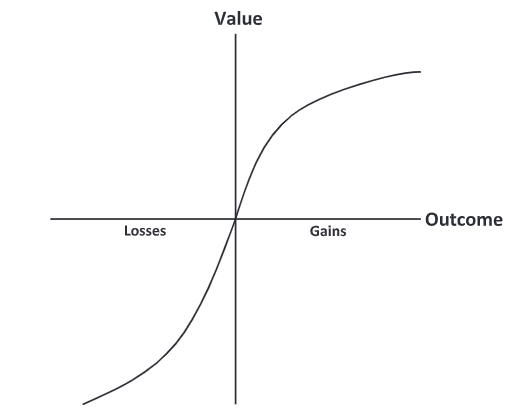
\includegraphics[width=7cm]{ValueFunction.PNG}
\caption[Representation of hypothetical value function]{Representation of hypothetical value function, based on \cite{prospect2}}
\label{Figure:value}
\end{figure}
\newline \noindent
Another aspect that needs further discussion in cumulative prospect theory is the so called probability weighting function. Based on their initial findings and later those of the rank-dependent utility theory, Kahneman and Tversky realized that people will not objectively perceive the probabilities of certain outcomes. This has been researched in many domains of psychology, beyond the applications of prospect theory \cite{Weighting}. In this work, the authors postulate that, as is the case in prospect theory, decision makers will not treat probabilities linearly. As can be seen in Figure \ref{Figure:weight}, the weighting function of a linear probability curve shows has an inverse-S-shaped evolution. 
\newline 
\begin{figure}[h!]
\centering
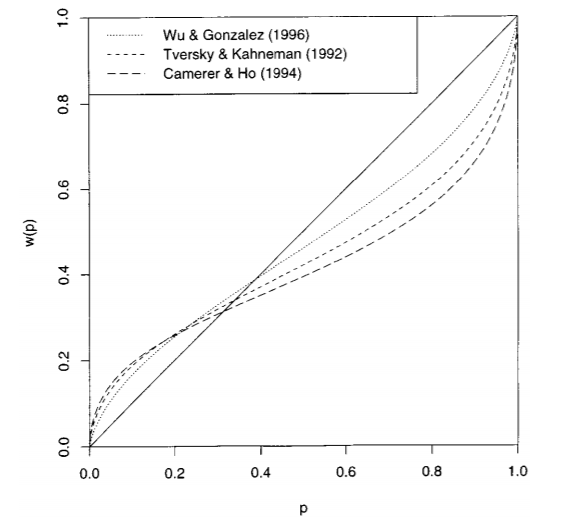
\includegraphics[width=8cm]{weighting-functions.png}
\caption[Representation of distorted weighting probability function]{Representation of distorted weighting probability function \cite{Weighting}}
\label{Figure:weight}
\end{figure}    
\newline
The evolution of this curve has been supported in several studies \cite{prospect2} \cite{Weighting2} \cite{Weighting3}. The probability weighting curve is concave for low probabilities (close to 0) and convex for higher probabilities (closer to 1). Intuitively, the evolution of this weighting function can be explained as the fact that people become less sensitive to changes in probability as this probability moves further away from the reference point. These reference point are the probabilities where a certain outcome 'is gonna happen for sure' or 'not going to happen at all', so 0 and 1. The evolution of the weighting function, therefore, will be more extreme when moving towards the reference point than when it moves towards the middle of the scale (probability of 0.4-0.6). Kahneman and Tversky referred to this effect as \textit{Diminishing Sensitivity}. The equation that satisfies this weighting function is:
\begin{equation}
    w^{+}(p) = \frac{p^{\gamma}}{(p^{\gamma} + (1-p)^{\gamma})^{1/\gamma}}
    \label{weight1}
\end{equation}
For positive prospects (i.e. when $x \geq 0$) and 
\begin{equation}
    w^{-}(p) = \frac{p^{\delta}}{(p^{\delta} + (1-p)^{\delta})^{1/\delta}}
    \label{weight2}
\end{equation}
\newline \newline \noindent
For negative prospects (i.e. when $x < 0$). The exponents $\gamma$ and $\delta$ have both been determined through extensive tests by Kahneman and Tversky. The value of $\gamma$ was found to be 0.61 and that of $\delta$ to be 0.69.
\newline \newline \noindent
With all the items of CPT known, a comparison with other behavioral economic theories can be done to determine if prospect theory is the more promising theory to model human behavior in investment decisions under risk. Nevertheless, two alternative decision making theories to prospect theory will be discussed, being expected utility theory (EUT) and rank dependent utility theory.
\subsection{\large{Related theories}}
As mentioned in section \ref{Prospect}, prospect theory is a continuation of different previously established behavioral economics models. In this section, therefore, these different theories will be highlighted. The most related are expected utility theory (EUT) and rank dependent utility theory.
\subsubsection{Expected utility theory} \label{EUT}
Like prospect theory, EUT is a theory to model decision making under risk. Rather than looking at the overall dollar value of a certain decision, EUT will consider the subjective value of a set of choices whose outcome is uncertain. Contrary to PT or CPT, the computation of the utility is very straightforward. Given a set of possible outcomes:
\begin{equation}
    (x_1,p_1;x_2,p_2;...;x_n,p_n)
\end{equation}
Then the expected utility can be calculated using the formula:
\begin{equation}
        E[u(x)] = \sum_{i=1}^{n}    p_i*u(x_i)
\end{equation}
According to EUT, agents will select the maximal utility of a set of possible choices. This computation, straightforward and easy to implement as it may seem, does make a few assumptions that make the theory unreliable and incomplete. The first one is the assumption that probabilities are perceived on a linear basis, which has been disproven by rank dependent utility theory, which will be discussed in the next subsection. In addition, as discussed in section \ref{Prospect}, the EUT fails to make good estimations of the certainty and reflection effect, estimations that were improved by PT. 
\newline \newline 
Despite being developed and postulated over two centuries before prospect theory (the foundations of EUT were laid by cousins Daniel and Nicolas Bernouilli in the so-called St-Peterburg Paradox in the first half of the 18th century \cite{Bernoulli}) and having been a widely accepted decision making model for a long time, recent efforts in behavioral economics have made the concepts proposed in EUT obsolete. This has already been proven in the literature \cite{EUTvsPT}. In this research, EUT and PT are compared as decision making models under risk in financial markets. The application of PT in this work is the so-called smooth prospect theory (SPT). The result from this work, where the authors simulated the behavior of agents populating an artificial market, were much more "realistically"  when using SPT compared to EUT. This already is a first indication that PT is the preferred candidate.
\subsubsection{Rank dependent utility theory}
This theory, developed as a response to the classical prospect theory by Kahneman and Tversky, is a generalised expected utility theory. The new ideas developed in this model were subsequently incorporated by Kahneman and Tversky in their cumulative prospect theory \cite{prospect2}. What makes rank dependent utility theory different from the general utility theory or the initial version of prospect theory, is the idea to introduce a cumulative probability distribution function of the outcome probabilities. This is contrary to using the individual probabilities to different outcomes \cite{rankdependent}. One of the main criticisms on PT that rank dependent utility theory tries to solve is the way the so-called first-order stochastic dominance\footnote{In statistics, a set \textit{F} first-order stochastically dominates a set G if a decision maker weakly prefers \textit{F} over \textit{G} for any weakly increasing utility function} was bypassed by Kahneman and Tversky. Aware of this problem, they introduced the editing phase into their PT \cite{prospect1}. This, however, had additional issues, like violations in transivity\footnote{A relationship \textit{R} over a set of variable {a,b,c} is said to be transitive if whenever \textit{R} relates to a and b and b and c, it also does so to a and c}.
\newline \newline \noindent
The rank-dependent model presented by Quiggin surpassed these issues by introducing transformations to the cumulative probability distribution function, rather than doing so to the probabilities of the outcomes. What Quiggin introduced, was the idea that outcomes with a very low likelihood of occuring will have a disproportionately perceived probability, whereas the probability of other, less extreme outcomes will be perceived normally. Since the innovations of the rank-dependent utility theory were later incorporated into the CPT, the latter theory can be concluded to be the most complete theory in behavioral economics for the modeling of decision making, which is the reason why it is the one that will be used for the remainder of this Thesis. 
\newline \newline \noindent
An overview of the different decision making theories can be found in table \ref{tab:overview1}.
\begin{table}[h!]
    \centering
    \begin{tabular}{||c|c|c|c||}
    \hline 
        \textbf{Theory}  & Flexibility & Complexity & Validity \\
    \hline \hline
         \textit{Expected utility} & Medium & Low & Low \\
    \hline
        \textit{Rank Dependent}  &  Medium & Medium & Medium\\
    \hline 
        \textit{Prospect}  & High & High & Medium\\
    \hline 
        \textit{Cumulative prospect}  & High & Medium & High\\
    \hline 
    \end{tabular}
    \caption{Overview decision making theories}
    \label{tab:overview1}
\end{table}
\subsection{Prospect theory in literature} \label{prospectliterature}
In the previous sections, the different aspects of behavioral economics and finance have first been discussed, followed by a description of the theories involved (prospect theory, expected utility theory and rank dependent utility theory). From this discussion, cumulative prospect theory (CPT) turns out to be the most suitable candidate to model investment decisions under risk. Since this Thesis focuses on investments in power generation and storage assets, it may be interesting to determine whether there has been related research. In doing so, it is important to consider that the research in this Thesis is on a household/prosumer level.  
%\newline \newline \noindent
%There has been research into the consumption-investment behavior of a household in more than one period \cite{Consumption}. In this work, the consumption and investment patterns of a household are analysed using prospect theory. The main purpose of the research is to determine how assets are being allocated, between the more risky ones and riskless ones, compared to the consumption of the household. 
%\newline \newline \noindent
%Prospect theory has also been applied in financial markets, investments and portfolio management\cite{portfoliochoice, portfoliochoicestat, portfoliochoicean}. In both works, cumulative prospect theory (CPT) is used for the optimal portfolio selection with one risk-free asset and one risky asset. This is done in a multi-period setting. In doing so, portfolio constraints are taken into account. In \cite{portfoliochoicestat}, the portfolio returns are static, whereas a stochastic process is imposed on them in \cite{portfoliochoice}. Through numerical simulations, all the different parameters are subsequently tested. In \cite{portfoliochoicean}, this test is done in an analytical manner. In some papers, the focus is rather on multiple assets rather than investments over multiple periods \cite{multistock}. In this work, prospect theory is used to model the investments in a single-period setting with one riskless bond and multiple stocks. From these works in financial markets, authors were able to spot a few trends. As the risk aversion of the agents increased, the proportion of wealth invested in risky assets as a function the entire portfolio increased in parallel. Moreover, the popularity of risky assets decreased as the returns of the assets decreased and/or the volatility of the assets increased. Something the authors of \cite{portfoliochoice} also observed was that the effect of changing risk aversion on the investment decisions in the different portfolio assets decreased over time.
%\newline \newline \noindent
%Besides the previously mentioned fields, prospect theory has also been used in different fields, like the modeling of the investments in spectrum for wireless communication \cite{spectrum}. In this research, the investment problem is defined as a two-stage investment to model the optimal investment strategy under the uncertainty of which actions to do on the spectrum market. In the case of this work, however, the application of prospect leads to a non-convex optimization problem, which brought an additional level of difficulty to the model. Contrary to classical prospect theory, however, the operator is both risk averse and loss averse. 
\newline \newline \noindent
Prospect theory has been used in energy research to model the behaviour of agents in domains like energy trading and storage investments \cite{Stackelbergprospect,Storageprospect,consumercentric,loadshift,reactive}. In \cite{Stackelbergprospect}, the interaction between a group of smart grid prosumers on the one hand and a power company on the other hand is studied. Here, the power company will act as a single leader, with multiple followers (this is also called a Stackelberg game). Prospect theory is used in the valuation of the utility of certain gains and losses for the prosumer. In addition, a comparison is made with game theory. In \cite{Storageprospect}, the interaction and exchange of energy of several distributed energy storage units. Prospect theory is used as an alternative to game theory, to make the decision less objective and rational. Since behavior of the operator of the storage unit will deviate from the optimal schedule, it is possible that some undesirable situations present themselves, like undesirable grid loads and revenues. This will cause the central power company to rethink their pricing scheme and the prosumers to change their charging and discharging habits. In \cite{consumercentric}, prospect theory is proposed as a decision-making framework to help understand how risk and uncertainty are perceived by smart grid consumers and how it will shape their investment decisions. In \cite{loadshift}, the same logic of irrational, non-optimal decision making is applied to load shifting in the context of demand-side management (DSM). Most of the work concerning DSM assumes agents will be objective and fully rational agents, which is an oversimplification this work tries to rephrase. In \cite{reactive}, finally, the authors attempt to apply the same logic to the valuation customers will perform of the compensation value for reactive power compensation. Contrary to most studies who let the agent optimize the objective value of the reactive power compensation value, this work lets agents optimize the subjective value of the reactive power compensation.  In the aforementioned works, the authors acknowledge that PT can increase the ability of simulating decision-making of actors in the energy market. They also claim the potential of PT is underdeveloped and will become a key modeling technique in the design and analysis of consumer-centric energy systems like smart grids. Considering this support for CPT in energy-related research, using this theory in the setting of this Thesis is permitted. 
\section{{Modeling Methods}} \label{Modeling}
\subsection{\large{Introduction}}
In this section, the different modeling techniques will be discussed that can be used for the simulation of investment decision in the electricity sector. First, the equation based models (optimization and equilibrium modeling) will be discussed, followed by the modeling technique that will be used in this dissertation, being agent-based modeling (ABM). In discussing the different modeling techniques, the focus will mainly be on their validity in modeling a human process that investing (usually)\footnote{Nowadays, many so-called quantitative hedge funds use computer models to invest in securities without any human intervention, sometimes with amazing results} is, especially in the context of this Thesis. This includes discussing their advantages as well as their shortcomings. 
\subsection{\large{Optimization modeling}}
The most traditional kind of modeling technique for decision making is optimization modeling \cite{optimization}. The basic premises for this technique is finding the best possible solution from a set of alternatives. Usually, there will be a finite amount of possible solutions to the problem, which is often referred to as the feasible region. Even if the model is formulated as a continuous problem, a computer solver will discretize the model, making the set of solutions limited. The size of the feasible region is limited by so called 'constraints', which are conditions imposed on the problem that limit the values that certain variables in the equations can have. Often, these constraints will be of a physical nature, like mass balances, temperature constraints or process efficiencies, to name a few.
\newline \newline \noindent
An optimization problem can mathematically be represented as an objective function that needs to be either maximized or minimized (like a cost function):
\begin{equation}
    {min/max}_{x} \; f(x)
\end{equation}
Where the feasible region is constrained by a set of equality constraints:
\begin{equation}
    h(x) = 0
\end{equation}
and inequality constraints:
\begin{equation}
    g(x) \leq 0
\end{equation}
Taking into account these boundary conditions, the optimal solution to this problem, which gives the maximal/minimum value of the objective function and corresponding parameter values, can be obtained. Often, the objective function and constraints will be a function of many process variables. The final optimization model can come in many different forms, like a linear problem (LP), non-linear problem (NLP), mixed-integer linear problem (MILP) and mixed-integer non-linear problem (MINLP), to name a few. To obtain the optimal solution of this set of objective function and (in)equality constraints, a multitude of solution methodologies are available, like the Newton-Rhapson method and steepest descent method for NLPs, just to name a few.
\newline \newline \noindent
Optimization is used in many different engineering processes, like chemical processes, thermal networks and electronic filter design, to name a few. In electricity investment decision models, this method has been considerably used in the past \cite{Optimization1,Optimization2,Optimization3}. This has gradually been substituted by other models, which shall be discussed in the next subsections. Since optimization modeling offers a rigid framework for the model formulation and follows a rigorous path to obtain a solution, it is a very accessible way to analyse a system and obtain an optimal solution. Once  the variables involved in a system are known, the objective that needs to optimized and the limitations of the system, the solution lies within reach. This makes it such a good candidate for the modeling of physical/chemical processes. For processes that involve human behavior, however, there are a few issues with this modeling technique. First of all, the optimization of a system implies that an actor has access to all information concerning the system, which rarely is the case in an investment decision process. Moreover, optimization modeling implies that the agent/decision maker will make choices on a rational basis. Both these assumptions, unfortunately, are oversimplifications of the complex process that investment decision making is. More complex modeling techniques like equilibrium modeling and agent-based modeling, which will be discussed later in this chapter, therefore, make it possible to capture these process complexities.  
%It must be noted, however, that although optimization modeling will not be the prevailing decision making technique in this Thesis, it will serve as a method to solve a "sub-problem" of the overall model. To calculate the optimal cost savings of a given PV-battery configuration, an optimization problem with certain boundary conditions will be formulated and used in the model. The objective function, constraints and solutions to this problem will be discussed in chapter 4, when the model development will be the main point of discussion. 
\subsection{\large{Equilibrium modeling}}
Whereas optimization modeling will strive to find the optimal solution of a certain set of equations, equilibrium modeling is a more specific technique to determine the equilibrium between different actors. This equilibrium can be competitive, cooperative or a leader-follower equilibrium, like a Stackelberg game. Equilibrium modeling, therefore, is more focused on economic optimization, whereas optimization modeling can be applied to any kind of process. In practice, therefore, different actors will perform an optimization of a certain system and make a decision from their point of view. Based on these optimality conditions, the equilibrium can be determined \cite{Poncelet}. This will be the point where the gains of all agents combined will be maximal. A common example is the equilibrium between the consumer and producer surplus in a supply-demand curve. The total surplus will be maximized by the different agents (consumers and producers) performing a personal optimization and choosing prices and quantities accordingly. A schematic overview of an equilibrium model can be found in Figure \ref{Figure:equi}. 
\begin{figure}[h!]
\centering
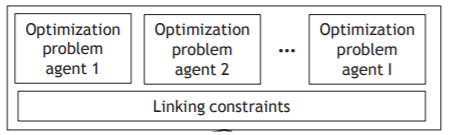
\includegraphics[width=10cm]{Equilibrium.PNG}
\caption[Graphical representation of an equilibrium model]{Graphical representation of an equilibrium model (source: \cite{Poncelet})}
\label{Figure:equi}
\end{figure}
\noindent
Besides the fact that this modeling technique will 'decentralise' the decision making process whereas optimization modeling has a centralised starting point, this modeling technique can incorporate market inefficiencies. Contrary to optimization modeling, this modeling technique can relax some assumptions regarding efficient markets, perfect information and rational decision making. It is, however, still an equation based modeling technique that will solve a set of processes towards an equilibrium, which makes it difficult to capture the dynamics of complex adaptive systems, which real-world systems often are. Since the focus in this Thesis is on the emergence of PV-battery adoption through economic utility and interaction between agents, equilibrium modeling may not be the best technique to model this adaptive process. Agent-based modeling, which will be discussed in the next subsection, will be able to capture the properties of CAS. 
\subsection{\large{Agent-based modeling}} \label{AgentBased}
The previously discussed modeling methods are able to solve a certain process (represented by a set of equations) and find its optimal configuration. This solution, however, is a 'static' solution. For a given set of equations, optimization and equilibrium modeling will find a unique solution to this problem. This methodology is useful in systems that strive towards a certain static state of optimal equilibrium, like heat transfer processes or chemical reactions. The modeling of CAS, where emergent, adaptive and self-organizing behavior of the agents, to name few, have to be accounted for, requires a more comprehensive modeling technique. This technique must be able to surpass the equation-based description of a certain process. ABM will be able to do that, by subjecting the agents in the CAS to a set of rules they must abide, in an attempt to create a more realistic simulation of a dynamic  phenomenon.
\newline \newline \noindent
Whereas advanced optimization and equilibrium models require large sets of equations to describe a system, agent based models will add an additional level of complexity to the description and simulation of these processes by moving away from a top-down system description (as is done in optimization and to a certain extent in equilibrium modeling). On the contrary, ABM's approach will be the exact opposite, by describing the system bottom-up in the form of behavior rules. This added level of complexity is introduced into the modeling approach to improve the descriptive capabilities of the model. The trade-off is the added level op complexity and computation time for ABMs. An ABM will consist of agents, who will dynamically interact with each other in their environment. Throughout the simulation of the agents' behavior in the environment, agent interaction will give rise to emergent properties on a system level. Note how this property is aligned with the emergent property of a CAS. ABM has a few advantages compared to the previously discussed techniques. Since the construction and simulation of the model are a bottom-up process, agent characteristic can be simulated, monitored and analysed more efficiently. When considering how the emergent properties of a system manifest themselves, as is the case in this Thesis, ABMs can be a very useful tool to visualise this emergence. Another advantage of ABM is the possibility to study the path dependence of a certain process. The 'trajectory' of the model over the course of its simulation period can be observed, providing valuable insights in the model dynamics of a system. Since optimization or equilibrium models will converge to a certain system or process equilibrium, this path dependence cannot be observed as easily. With any advantage also comes a disadvantage, which in the case of ABM is modularity. Since this modeling technique can be applied in a wide range of applications to describe and simulate the behavior of CAS, ABM will not have a standard framework like optimization modeling to formulate and solve the model. The developer of an ABM, therefore, must pay close attention to the characteristics and important parameters of the system to formalise these into a well functioning model. A good understanding of the underlying principles of a model are necessary to ensure a good development of an ABM.
\newline \newline \noindent
This modeling technique, therefore, will serve as the technique to simulate the investment decisions in DERs on a household level. An overview of the different modeling techniques can be found in table \ref{tab:overview2}.
\begin{table}[h!]
    \centering
    \begin{tabular}{||c|c|c|c|c||}
    \hline 
        \textbf{Modeling technique} & Framework & Flexibility & Complexity & Validity \\
    \hline \hline
         \textit{Optimization modeling} & Standard & Medium & Medium & Low \\
    \hline
        \textit{Equilibrium modeling} & Standard &  High & Medium & Medium\\
    \hline 
        \textit{Agent-based modeling} & Modular & High & High & High\\
    \hline 
    \end{tabular}
    \caption{Overview modeling techniques}
    \label{tab:overview2}
\end{table}
Contrary to the optimization and equilibrium modeling techniques, which have a standard framework to formulate the model and generate a solution, the agent-based modeling method requires a more modular approach. As is the case in this Thesis, optimization models and other theories (like CPT or EUT) will be used as building blocks of the overall ABM (see Chapter 4). By combining all these building blocks with respect to agent properties and system interaction, a comprehensive model can be developed. This can make the model description more realistic, but it also requires a thorough understanding of the system under consideration.
\section{Research approach} \label{approach}
The system description in this Thesis relies on CAS theory. The underlying theory can help identify these elements, as well as the relationships among those elements that need to be considered for the analysis and description of a CAS. One of those elements (i.e., adaptation) is described by using the concepts of prospect theory. The most recent version of prospect theory, being the CPT, will be used to that end. 
\newline \newline \noindent
The concept of adaption is further formalized by using prospect theory. Since adaptation in the model is a change in the means of electricity production for the household, the adaptation will translate itself in the adoption of DERs of PV-battery systems. The simulation of this adoption process will be accounted for using CPT, which will subsequently become part of the ABM. The other components of the CAS, being emergence and state-based responses, will be directly embedded in the ABM. A conceptual overview of the model approach can be seen in Figure \ref{Figure:approach}.
\newline 
\begin{figure}[h!]
\centering
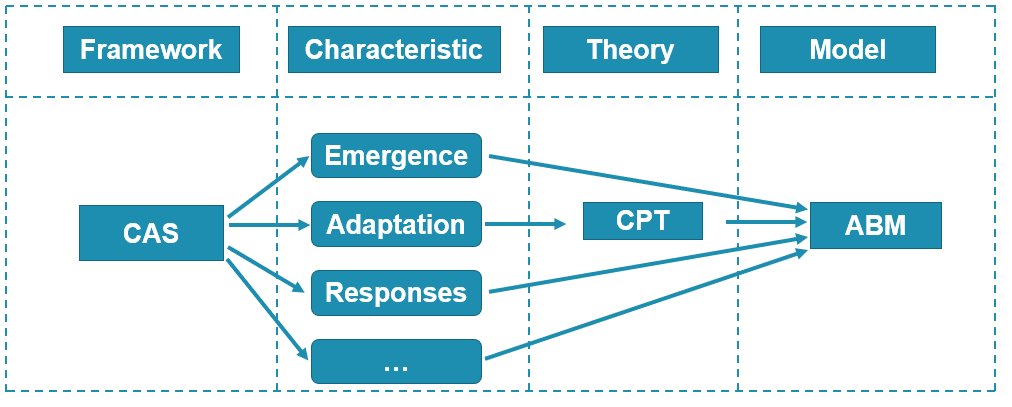
\includegraphics[width=10cm]{approach.PNG}
\caption{Graphical representation of modeling approach}
\label{Figure:approach}
\end{figure}
\newline \noindent
A detailed description of the how these concepts were formalized into an ABM will be the main point of focus in Chapter 4.
\chapter{Model Design}
\section{Introduction}
In this section, the theories and methods from Chapter 3 will be formalized into a computational model. Before doing so, the characteristics of the system under consideration will be discussed. The model will simulate the behavior of agents in a consumer-centric energy system. Section \ref{CASEnergy} will discuss whether this consumer-centric energy system is a CAS or not. Since the model is rather complex due to the large amount of agents and interactions, the explanation of the model will be done in different stages. In section \ref{Concept}, the logical process that created the final version of the model will be summarized. Since the model development happened through a few important stages, between which features got added and complexity gradually increased, an conceptual overview of these different steps will help the reader in understanding the final version of the model. In this section, the description of the model will be limited to a high-level overview of the input parameters, output parameters and agents in the environment. A more detailed description of the model will be discussed in section \ref{formalisation}. In this section, the different processes, equations and input data included in the model will be described by using the ODD protocol\footnote{The ODD protocol is a framework developed specifically for agent-based model to describe and decompose the ABM in a systematic and standardised manner}. This standard structure called the ODD protocol will be followed to make the system decomposition as straightforward and reproducible as possible.
\section{Consumer-centric energy system as a complex adaptive system?} \label{CASEnergy}
One of the main assumptions of this Thesis is that a consumer-centric energy system can be considered a complex adaptive system. This assumption can be supported by comparing the properties of a CAS with the system under consideration. First, however, the layout of the system must be presented.
\newline \newline \noindent
The system under consideration consists of a set of households and the DSO. Among the households, that are the electricity consumers, there will be two distinct groups: households that have the possibility to adopt DERs ("Replacement demand") and households that are not in the ability to adopt DERs due to logistical (i.e. households that live in apartment buildings or very remote places) or other constraints ("Residual demand"). The DSO will interact with both these groups, as can be seen in Figure \ref{Figure:split}.  
\begin{figure}[h!]
\centering
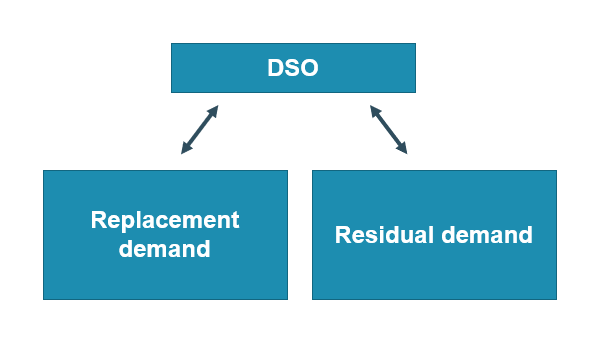
\includegraphics[width=8cm]{modelarge.PNG}
\caption{System overview}
\label{Figure:split}
\end{figure}
\noindent 
There will be multiple kinds of interactions in this system. These interactions will be both between the household with replacement demand as well as between the groups of households and the DSO. 
\newline \newline \noindent
The households with replacement demand will gradually adopt PV-battery configurations, driven by economic incentives and peer influences. The aggregate effect of all these agent-level adoptions will cause the overall DERs adoption levels to increase on a system level. This phenomenon is an form of emergent behavior, which is one of the most important characteristics of a CAS. The agents in the system will change their behavior based on changes in circumstantial factors. Households will change their attitude towards investing in DERs as the electricity price (including distribution cost), technology cost and peer influence change. The DSO will change its pricing strategy as the amount of electricity consumed will change. These changes will be an expression of adaptive characteristics on behalf of the agents. This adaptive behavior also is a cornerstone of any CAS and is very much present in the system under consideration. Since this Thesis studies the effect of different policies on the adoption of DERs and the utility death spiral, different stimuli will be introduced into the system which will influence the responses of the agents. Since these responses depend on the state a certain agent is in (wealth level, adoption characteristic, distribution tariff etc.), the responses are state-based responses. This also is an important part of a CAS.
\newline \newline \noindent
Since some of the most important characteristics of a CAS (emergence, adaption and state-based responses) will prevail in the system under consideration, it is a fair assumption to say that the energy system that the model simulates is a CAS. 
\section{Conceptual model} \label{Concept}
In this section, the model will be presented from a conceptual point of view, by gradually adding features to understand what the input-output relations of relevance are in the model. The end model of this Thesis is the result of many iterations of feature additions and intermediate evaluations, of which the final iteration will be the main point of attention in this section. A representation of this conceptual model can be found in Figure \ref{Figure:model3}.
%\begin{figure}[h!]
%\centering
%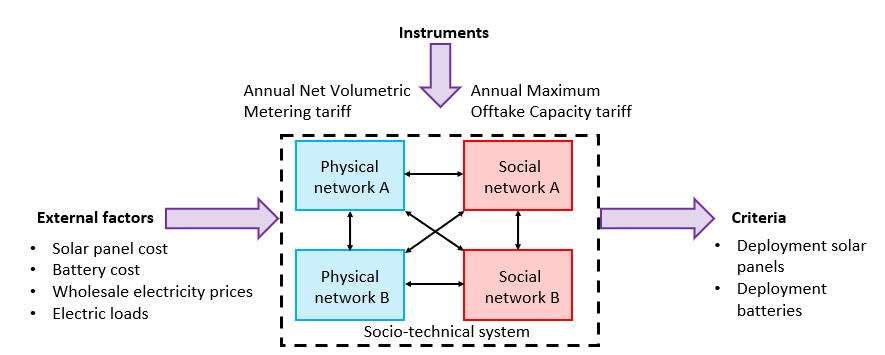
\includegraphics[width=10cm]{model1.PNG}
%\caption{Exogenous model overview}
%\label{Figure:model1}
%\end{figure}
%The independent variables are the different distribution tariffs that can be set by the grid operator. The first kind of distribution tariff is the net volumetric metering tariff. This tariff, which charges the electricity consumer a fixed distribution rate for each unit of net electricity taken from the grid, is the most common way DSOs will charge the end consumers for the usage of the distribution infrastructure. A common tariff charge is about 0.1\EUR{}/\textit{kWh}. Compared to the energy component of the overall electricity bill, this distribution cost will often be larger than the actual energy cost. 
%Another distribution tariff is the annual maximum offtake capacity tariff. For this tariff, the overall distribution cost will depend on the maximum demand on an annual basis. A common tariff charge for the capacity offtake tariff is about 9.0 \EUR{}/$kW_{peak}$. 
%\newline \newline \noindent
%Since the distribution tariffs are exogenous in this stage of the model, they remain constant throughout the simulation period. Given all these input parameters, the battery and solar PV adoption will be the output parameters. In a next stage, the interaction between the households and the DSO will be added to the model, by making the group of households interact with the DSO. A visual representation of this model can be found in Figure \ref{Figure:model2}.
%\begin{figure}[h!]
%\centering
%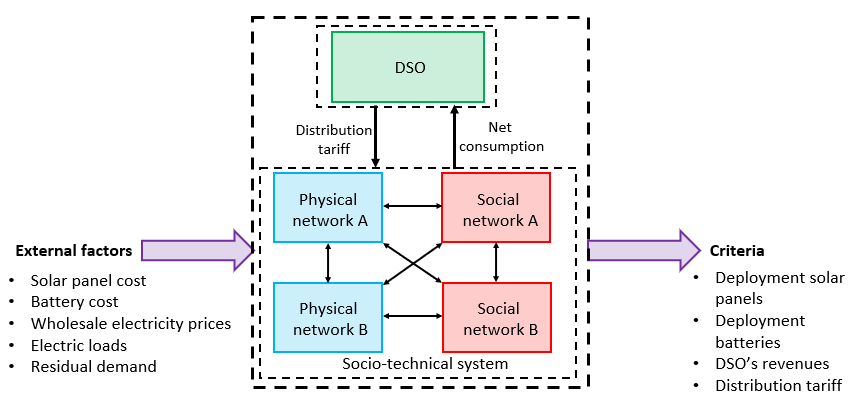
\includegraphics[width=10cm]{model2.PNG}
%\caption{Endogenous model overview}
%\label{Figure:model2}
%\end{figure}
%In addition to the aforementioned input parameters, the residual load will also have to be explicitly defined. This parameter is required to determine the extent of the utility death spiral. The distribution tariffs no longer will be constant, but their initial values will still need to be defined. As the PV and battery adoption increases and the electricity demand from the grid changes over time, the DSO will see a shift in his revenues, forcing him to adapt his pricing towards the end customers. The output parameters in this version of the model, therefore, next to the PV and battery adoption are the DSO revenues and distribution tariffs. 
%\newline \newline \noindent
%In the final version of the model, the represented model of Figure \ref{Figure:model2} is to be tested for different policies, as can be seen in Figure \ref{Figure:model3}. The policies that are to be evaluated are the feed-in tariff, net metering, net billing and battery subsidies. The data used to quantify these different adoption incentives was based on those policies being deployed in Belgium. 
\begin{figure}[h!]
\centering
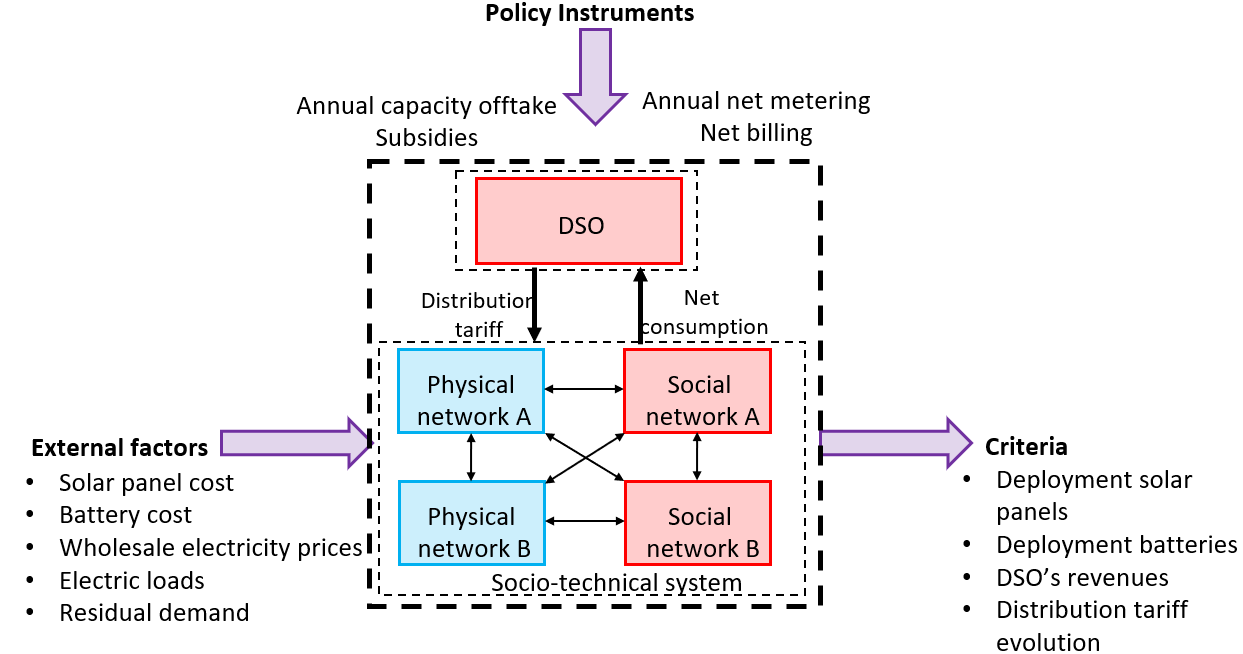
\includegraphics[width=10cm]{model3.PNG}
\caption{Policy model overview}
\label{Figure:model3}
\end{figure}
As can be seen, the exogenous input parameters to the model are the different policies considered in the Thesis: annual net metering, annual capacity offtake, net billing and battery subsidies. The external input parameters are the solar panel cost, battery cost, wholesale electricity price, electric load and residual demand of the aggregate of households. The resulting output parameters are the solar PV deployment, battery deployment and the evolution of the distribution tariff.  
\section{Model formalisation} \label{formalisation}
\subsection{Introduction}
In this section, the theories and methods that were discussed in section \ref{Prospect} and section \ref{Modeling} will be used to develop the agent-based model for simulating the DERs adoption on a household level. In doing so, a common framework for the decomposition of ABM, called the ODD framework, will be the first point of attention.
\subsection{ODD protocol}
Due to the complexity of some ABMs, a standard framework for the description of these models is a useful way to understand, decompose and reuse a model, or parts of it. The ODD protocol can serve as a structure to fulfill this task. The ODD (acronym for 'Overview', 'Design Concepts' and 'Details') is a protocol that was developed to standardize the description of agent-based and individual-based models in publications. This way, models are easier to understand and implement in later research. Within the three basic elements of the ODD protocol, there are a few sub-elements that have to be defined. Before going to the specific model development in section \ref{MODEL}, a description of the ODD protocol will be given. The sub-elements of the ODD protocol are: 
\begin{itemize}
    \item \textbf{Overview}: Purpose, entities/state variables/scales and process overview/scheduling. 
    \item \textbf{Design concepts}: Basic principles, emergence, adaptation, objectives, learning, prediction, sensing, interaction, stochasticity, collectives and observation.
    \item \textbf{Details}: Initialization, input data and submodels.
\end{itemize}
By addressing the different topics in this framework, the structure of the model under consideration can be decomposed and reported. Since the model simulates the behavior of agents in a CAS, the different characteristics discussed in section \ref{CAS} will also be a point of attention. Therefore, the different items characterizing CAS and the different parts of the ODD framework will be aligned in section \ref{development}.
\subsection{Model development} \label{MODEL} \label{development}
Concepts from CAS theory and decision making theories will now be formalized into an agent-based model. A first point of attention will be the assumptions governing the model. Subsequently, the model overview will be presented according to the items of the ODD protocol and discussing how the different characteristics of CAS theory fit into this model description. 
\subsubsection{Assumptions}
The following assumptions were made in the development of the model:
\begin{itemize} 
    \item Besides the energy and distribution component, no other parts to the electricity cost (like taxes and levies) are considered.
    \item The households will be risk seeking when facing losses and risk averse when facing gains.
    \item The households will act as prospect value-maximizing agents (subjective value optimization).            
    \item Several data sequences, like the DAM electricity prices and the load factor of the PV are exogenous. The load factor remains constant throughout the entire temporal scope of the model.
    \item The agents/households live densely enough to be able to observe what their neighbors are doing. If this was not the case, the influence of the peer effect could no longer be relied upon.
    \item The interaction between the aggregate of households and the DSO is assumed to be direct without any intermediary party like an aggregator or flexibility service provider.
    \item The nature of the household remains unchanged over time: an innovator remains an innovator throughout the entire simulation, as will laggards and all the other classes of households.
    \item The financing of the DERs is done entirely through the own means of the household. Given the very low interest rates that have been shaping the financial markets in past years, debt is virtually free and, therefore, this is a fair assumption \cite{ECB}.
     \item The households adopt on a one-off basis, meaning that no upgrades or extensions of the adopted configurations are possible.
     \item Since the focus in this Thesis is on the adoption of DERs rather than the decommissioning, the latter is not accounted for in the model.
     \item The residual load households' demand elasticity to the electricity price is assumed to be 0. This implies that for increasing network charges and electricity cost, the residential demand of these households remains the same. 
\end{itemize}
With these assumptions in mind, the model will be described using the ODD protocol, which will be done in the next section.
\subsubsection{Model Overview} \label{overview}
In this section, the ODD protocol will be used to describe the model that simulates households' DERs adoption. When discussing the different characteristics and components of the model, their relevance in the CAS framework, which was discussed in section \ref{CAS}, will also be a point OF attention.
\begin{itemize}
 %   \item \textbf{Purpose}: provide insights into how different policy instruments, like net billing, net metering, feed-in tariffs and others affect household DERs adoption and enhance the utility death spiral.
   % \item \textit{Entities}:  different agents, being the different households and the DSO
   % \item \textbf{State variables}: adoption rates of PV/Battery systems, income level and adoption type for the households. For the DSO, these state variables are the distribution tariffs and grid revenues
    %\item \textbf{Scale}: The temporal scale is 20 years (lifetime of the technology under investigation). The temporal resolution of the model is 1 year. The spatial specification are also necessary since this model will consider the peer effects of the households upon each other
   % \item \textbf{Project overview}:  describes the schedule of the different processes in the model. A high level description of the process overview can be seen in Figure \ref{fig:flow}. The underlying models that will require further discussion are the cost optimization model, the economic utility calculation, peer adoption effect (and social utility calculation) and distribution tariff variation. This part of the model discussion can be found in section \ref{submodel}. 
   % \newline 
   % \begin{figure}[h!]
        %\centering
        %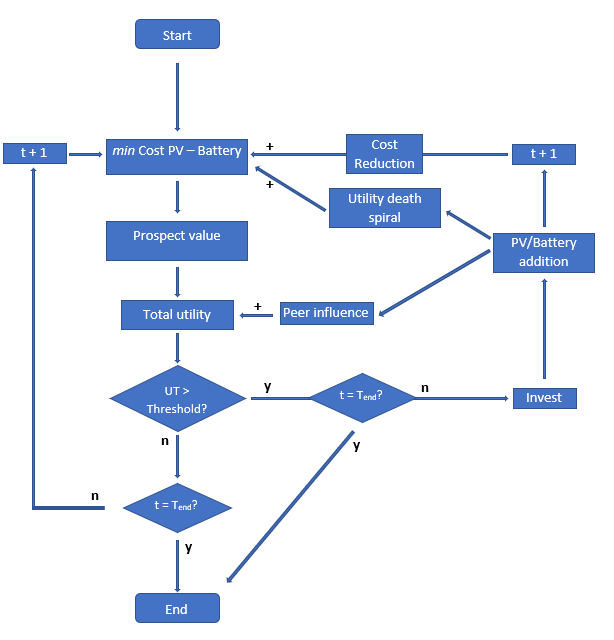
\includegraphics[width=10cm]{flowchart.PNG}
      %  \caption{Process overview of the model}
    %    \label{fig:flow}
  %  \end{figure}
    %\item \textbf{basic principles} are the implementation of cumulative prospect theory into an investment decision making model for DERs on a household level.
    %\item \textbf{emergent behavior} since the aggregate of households will gradually adopt PV-battery configurations, initially due to purely economic reasons, but gradually also due to the social utility that the peer effect will evoke.
\end{itemize}
%\newline \newline \noindent
The \textbf{purpose} of the model in this Thesis is to provide insights into how different policy instruments, like net billing, net metering and battery subsidies affect household DERs adoption and enhance the utility death spiral. In the model, the adoption of DERs, PV/battery configurations to be more specific, is simulated on a household level. The system the model considers consists of a group of several thousands of households that will interact with each other through the peer effect. Combining the social utility of this peer effect with their economic utility, households will decide whether to adopt DERs or not. The group of households will also interact with the DSO through the variation of distribution tariffs due to less electricity consumption from the grid after having adopted DERs.
\newline \newline \noindent
The \textbf{entities} of the model are the different agents, being the different households and the DSO. The \textbf{state variables} are the adoption rates of PV/Battery systems, income level and adoption type for the households. For the DSO, these state variables are the distribution tariffs and grid revenues. The \textbf{scales} of the model are both temporal and spatial. The temporal scale is 40 years (lifetime of the technology under investigation). The temporal resolution of the model is 1 year. The spatial specification are also necessary since this model will consider the peer effects of the households upon each other. The spatial scale, therefore, must be confined to an area consisting of a group of households of sufficient size to make the effects of the adoption clearly visible. This household network will be modeled using the income level distribution of the households. The \textbf{process overview} describes the schedule of the different processes in the model. A high level description of the process overview can be seen in Figure \ref{fig:flow}. The underlying models that will require further discussion are the cost optimization model, the economic utility calculation, peer adoption effect and distribution tariff variation. This part of the model discussion can be found in section \ref{submodel}. 
\newline 
\begin{figure}[h!]
    \centering
    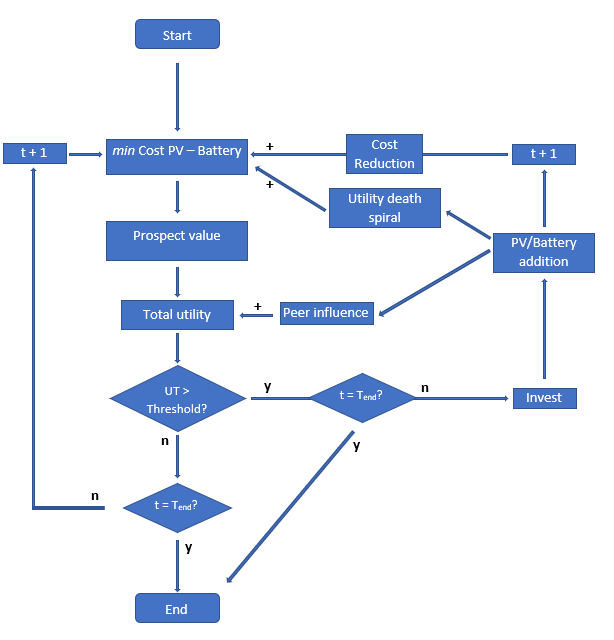
\includegraphics[width=10cm]{flowchart.PNG}
    \caption{Process overview of the model}
    \label{fig:flow}
\end{figure}
\noindent
When focusing more on the design concepts, the \textbf{basic principles} are the implementation of cumulative prospect theory into an investment decision making model for DERs on a household level. In doing so, the assumption is that individuals or households will not make decisions on a rational basis, but will incorporate risk aversion factors in their decision making. This model will incorporated into an agent-based model to describe the investment decision making in electricity generation assets. Prospect theory is used to capture non-rational behavior of households/individuals. In addition, social utility is also added in the utility calculation to account for non-economic decision variables. 
\newline \newline \noindent
Each agent will adapt his behavior to the situation at hand. Two parameters will cause the households to adapt their behavior: the economics of the technology and the peer effect. If the technology, be that PV or batteries, becomes cheaper because of further scaling or innovation, the utility of a certain configuration will increase, thereby causing the household to change its views on the technology, making its behavior change. If, on the other hand, many neighbors of a certain household adopt PV/battery installations, the peer effect will cause the social utility to increase, making the non-adopting households change their views on the adoption of the DERs, thereby making them adapt their behavior. The DSO will gradually adapt his behavior (by adapting the distribution tariffs) as the adoption of DERs increases and the utility death spiral starts manifesting itself. Note that this adaptation is very important in the overall ODD protocol, since it is one of the core characteristics of a CAS (see section \ref{CAS}). 
\newline \newline \noindent
Another  important characteristics of the CAS, emergent responses, will be present in the model. The model will show \textbf{emergent behavior} since the aggregate of households will gradually adopt PV-battery configurations, initially due to purely economic reasons, but gradually also due to the social utility that the peer effect will evoke. However, since the amount of households and installable capacity is limited, this emergent behavior in the model will saturate to a certain point, which will be a point of widescale PV adoption when sudden emergence of PV adoption no longer is possible. The agents in the system will show a different behavior towards their adoption patterns. Whereas the adoption will at first purely be motivated by economic utility, this will gradually become motivated by both economic and social utility.
\newline \newline \noindent
The \textbf{objectives} of the agents in the model will depend on what kind of agent is being considered. The objectives of the households are to minimize the costs (or under behavioral finance, the 'perceived cost') of  electricity consumption. For the DSO, the objective is to recover the costs it had to incur to construct and maintain his infrastructure. Although the agents in the model will show an adaptive behavior, there will be no additional \textbf{learning} features exhibited by the households other than the adaptations to the situation as it presents itself at any given moment in time. 
\newline \newline \noindent 
Another important property of a CAS (see section \ref{CAS}) is prediction. The \textbf{predictive} capacities of the households will also be limited, since all they do is predict what the NPV and payback period is of the PV/battery configuration. The different agents in the system will \textbf{sense} different parameters. The behavior of the agents will be influenced by the electricity prices (including the distribution costs), the load factor of the PV and the adoption of PV by the neighbors of the agent. The DSO will adapts his behavior according to the net amount of electricity that will be drawn from the grid and the residual demand (i.e. demand that cannot be substituted by PV or another DERs). 
\newline \newline \noindent
Agents will \textbf{interact} with each other. If more agents decide to adopt PV, thereby reducing the net demand for electricity, the DSO will react by increasing the distribution tariff on the electricity sold. In this process, the different agents are interacting with each other (i.e. they will adapt their behavior as a reaction to what other agents do). The households, however, will also interact with each other. Due to the peer effect, the adoption by other households becomes more likely if a neighboring households installs a PV-battery system. 
\newline \newline \noindent
Since there is a level of uncertainty created in some variable, like the price of electricity, load factor, or price of the technology, this model does integrate some \textbf{stochastic} processes. This uncertainty is incorporated through the projection of various random scenarios of different parameters. Therefore, the discussion of model simulation results will not be done using those of a single simulation. Rather, a Monte Carlo approach will be done to systematically analyze the results of a large batch of results, to get as complete a picture as possible of the internal mechanics of the model. This will require some computation time, but will give a more adequate representation of the model results. As mentioned earlier, there are several agent interactions in the system (i.e. household-household and household-DSO). Note how this visualisation aspect aligns with the computer simulation characteristics of the CAS (see section \ref{CAS})
\newline \newline \noindent
In the interaction between the group of households and the DSO in the utility death spiral, the households form an aggregation of agents that will collectively affect the state and behavior of the system, since the distribution tariff will be adapted through this \textbf{collective} behavior. To evaluate the model, the \textbf{observation} parameters will depend on the agent in the system. When looking at the households, the important parameters are the PV and battery adoption, social and total utility and the payback period of the technology, as well as the evolution of the NPV. On a system level, the PV and battery adoption levels are also an important observation parameter. For the DSO, the relevant parameters are the distribution tariff and the change in its revenue stream. 
\newline \newline \noindent
The model was \textbf{initialized} as follows: no households with any DERs, all electricity consumption from the grid and a volumetric or capacity distribution tariff. These initial conditions could also be changed to a partial adoption initial condition (for instance  30\% adoption of solar PV in a neighborhood), but since the focus in this Thesis is on the adoption process of the DERs, it is more interesting to simulate the entire adoption from scratch. The primary \textbf{input data} of the model should be the electricity price of the Day-ahead market (DAM) (Figure \ref{fig:price}) and the residential demand (Figure \ref{fig:demand}). 
%\begin{figure}[h!]
%\centering
%\begin{subfigure}{\textwidth}
%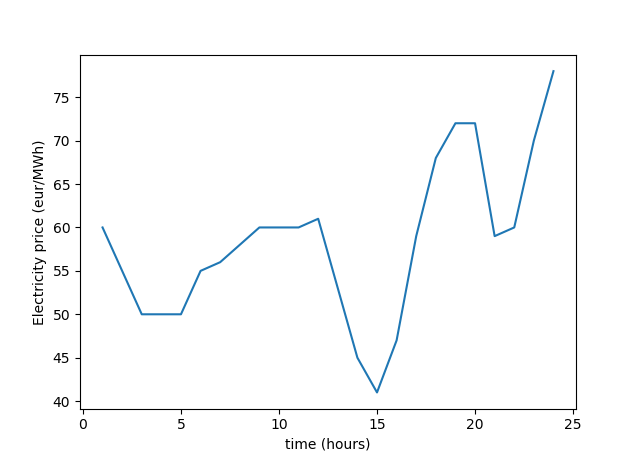
\includegraphics[width=7cm]{price.png}
%    \caption{DAM electricity price (\EUR{}/MWh)}
%    \label{fig:price}
%    \end{subfigure}
%\begin{subfigure}{\textwidth}
%    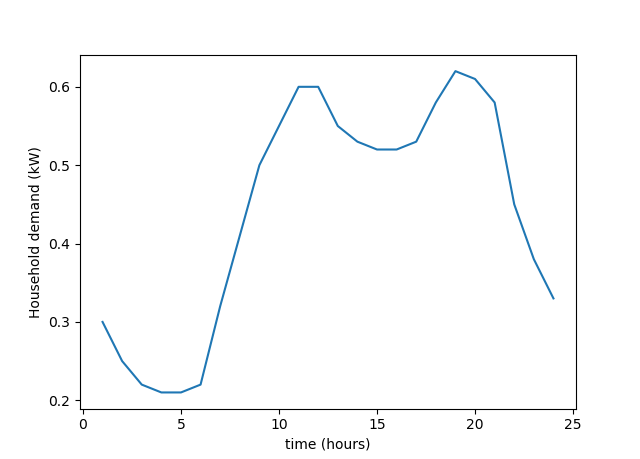
\includegraphics[width=7cm]{Demand.png}
%    \caption{Residential load profile (kW)}
%    \label{fig:demand}
%\end{subfigure}
%\label{fig:fig}
%\end{figure}
%\noindent
So far though, households are not charged hourly electricity prices. Usually, households are charged two tariffs: a night and day one. In all these cases, though, it is important to stress that varying price profiles could make the results of this model deviate from their intended purpose. The main focus of this Thesis is to determine how PV adoption and the utility death spiral occur as a result of economic and social incentives. By introducing sources of noise into the model, which can come in the form of varying electricity prices, varying PV prices or any other, therefore, it becomes increasingly difficult to observe the input-output relations of the model. Hourly electricity prices on a residential level could incentivize the households to adopt PV-batteries with the sole purpose of doing energy arbitrage between peak and low demand hours, rather than the economic and social incentives that are considered in this model. To avoid this hidden adoption incentive, electricity prices will assumed to be constant throughout an entire year. The price can still change in between years. If in the future hourly electricity prices are to be charged to households, this additional phenomenon will have to be accounted for in future work. 
\newline \newline \noindent
Since this model also concerns a PV system, the load factor also is an important set of input data. A representation of the load factor data that is to be used in this model can be found in Figure \ref{fig:LF}:
%\begin{figure}[h!]
%    \centering
%    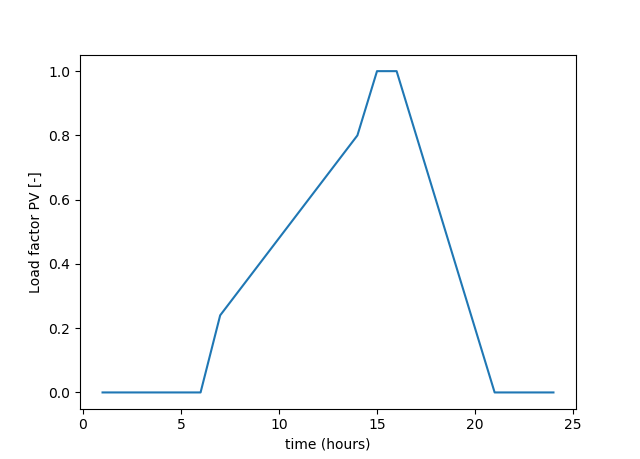
\includegraphics[width=7cm]{LF.png}
%    \caption{Load factor of the PV [-]}
%    \label{fig:LF}
%\end{figure}
%\noindent
The data shown in Figures \ref{fig:price},  \ref{fig:demand} and \ref{fig:LF} is a weighted average of a set of representative days to account for the annual profile of the residential demand, DAM electricity price and load factor. Using twelve standard profiles that jointly represent the most important characteristics of an annual electricity price, residential demand and PV load factor profile. Each of these days will have a representative weight to account for the annual profile. When performing calculations with this data, the amount of computations will remain limited, since the results of the calculations using representative days data can be multiplied with the associated weight, rather than performing the calculations with the entire annual data. An important side note to the data in Figure \ref{fig:demand} is that this data will vary as a function of the income/wealth of the household, which will be discussed in a subsequent paragraph.
\newline \newline \noindent
In addition to the exogenous data strings represented in Figures  \ref{fig:price}, \ref{fig:demand} and \ref{fig:LF}, some additional data will be required. The first important set of data is related to the technology cost. Since these technologies are also emerging technologies that are undergoing decreases in capital cost (see section \ref{Trends}), the assumed annual price decrease also is an important factor that should be included. This data can be found in table \ref{tab:PVbat}. The solar panel data on capital and operational costs can be found from the IEA data in Table \ref{table:1}. The value for the EU will be selected for the solar PV data: $\$1,300$ per $kW$.  The complementary maintenance cost will be included ($\$20$ per \textit{kW}). The battery data comes from the cost estimaetes by the NREL \cite{batdata}. On average, the cost of the battery is 500 $\frac{\$}{kWh}$.
\begin{table}[h!]
    \centering
    \begin{tabular}{||c|c|c|c||}
    \hline 
          \textit{\textbf{Technology}} & \textit{Capex} ($\frac{\$}{kW(h)}$) & \textit{Opex} ($\frac{\$}{kW(h)-year}$) & \textit{Capex decrease} (\%)\\
         \hline 
         \hline
          \textbf{\textbf{PV}} & 1,300 & 10 & 3\\
          \textbf{\textbf{Battery}} & 500 & 9 & 5\\
          \hline 
    \end{tabular}
    \caption{Cost overview of PV \& battery}
    \label{tab:PVbat}
\end{table}
The capital costs of the PV are assumed to decrease by 3\%,. This value is the result of an estimation based on the capital cost decrease projection of the PV in Table \ref{table:1}: the capital cost is expected to decrease by 41\% by 2040, which results in an annual cost decrease of 2.5 - 3\%. Cost decreases for residential storage facilities are more challenging to obtain, but since this technology will still undergo a substantial expansion, the annual cost decrease is going to be higher. In this Thesis, a cost decrease of 5\% is assumed. This may appear to be a high value, but when comparing this to the annual cost decrease for the lithium-ion technology in recent years (see Figure \ref{Figure:bloom}), this cost decrease seems reasonable. One point of attention that must be met here, however, is that this cost decrease of PV and battery technology hinges on the ability of the DER manufacturers to keep up with this demand. The overall demand for PV is expected to steadily increase the cumulative PV capacity (see Figure \ref{Figure:PVfut}), but if this demand systematically exhaust the limited supply, the cost of PV and other DER will no longer decrease as projected. Depending on the evolution of the PV manufacturers, this assumption will have to be adjusted in the future. 
\newline \newline \noindent
The additional costs the households will have to incur for the installation of the PV-battery system include the cost of the converter, cables, protective equipment and installation labour cost. For each configuration, this cost is assumed to be fixed (\EUR{}1200\footnote{Based on the recent installation of PV panels at the authors' home}). With all the different cost components known, there will be a set of available configurations. In reality, there are many possible configurations for households to adopt. Selecting a PV-battery configuration, nonetheless, is always a discrete process, since both PV panels and batteries come in modules of some minimal capacity. The possible configuration can, therefore, be approximated by a limited set of options, as can be seen in table \ref{tab:config}.
\begin{table}[h!]
    \centering
    \begin{tabular}{||c|c|c||}
    \hline 
          \textbf{\textit{Option}} & \textit{PV capacity} $(kW_p)$ & \textit{Battery capacity} $(kWh)$\\
         \hline 
         \hline
          1 & 1.5 & 0.0\\
          2 & 1.5 & 2.0\\
          3 & 2.5 & 0.0\\
          4 & 2.5 & 2.0\\
          5 & 4.0 & 0.0\\
          6 & 4.0 & 2.0\\
          7 & 4.0 & 5.0\\
          \hline
    \end{tabular}
    \caption{Overview of PV-battery configurations}
    \label{tab:config}
\end{table}
Note how for each of the PV sizes, there will be the possibility of adopting both a PV with or without battery (of \textit{2.0 kWh}). For the largest PV system, there will also be the possibility to adopt a larger battery of \textit{5.0 kWh}. Each household will have to choose from one of these configurations when it wants to invest. This set of options is, of course, very limited. In reality, the number of possible configurations will be larger, but not extremely large, since the decision process in PV-battery systems will always be a bit of a discrete process. 
\newline \newline \noindent
The maximal charging/discharging power of the batteries can be determined by looking at different options available. By examining the different options laid out by Clean Energy Reviews, the maximal power output of residential batteries is roughly equal to $0.5*E_{BAT}$ \cite{batpower}. The charging power will, therefore, be $1.0kW$ for the $2.0 kWh$ battery and $2.5 kW$ for the $5.0 kWh$ battery. As a final note, no self-leakage and discharge losses are assumed. 	
\newline \newline \noindent
As was discussed earlier, the demand of the households will depend on the levels of wealth of the household. In Figure \ref{fig:wealth} the estimated financial wealth distribution of all households in Belgium can be seen. This data was estimated by combining the financial wealth of the individuals in Belgium and the distribution between different population classes \cite{wealthdata,wealthdata2}. According to this distribution, the demand will deviate from the data presented in Figure \ref{fig:demand}.
\begin{figure}[h!]
    \centering
    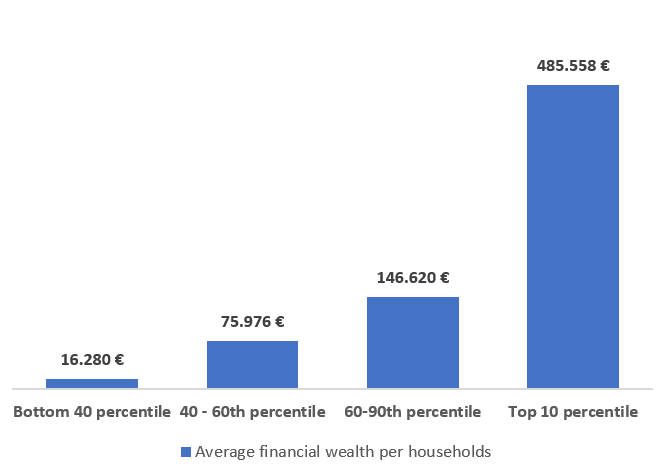
\includegraphics[width=8cm]{incomedist.PNG}
    \caption[Distribution of financial wealth]{Distribution of financial wealth \cite{wealthdata,wealthdata2}}
    \label{fig:wealth}
\end{figure}
\newline
The lowest wealth class, which accounts for 40\% of the overall population, is assumed to have a demand profile like Figure \ref{fig:demand}, only at a 20\% lower average. The subsequent wealth class, accounting for a fifth of the overall population (40-60\%), is assumed to have a demand profile that corresponds exactly to the one in Figure \ref{fig:demand}. The second to last income class, accounting for the 60th to 90th percentile of the wealth distribution, will have a demand profile that is on average 20\% higher than the standard one. The final wealth class, being the final 10\% of all the households, will have a demand profile 50\% higher than the average profile. Besides a distribution according to income, the households will also be classified according to their willingness to innovate, which will be discussed in Section \ref{submodel}. Note that this assumption is only valid if the household size is uniform (i.e., each households has the same number of members). In reality, however, poorer households tend to have more members, causing their aggregate electricity demand to be larger. This level of granularity in the household data, however, is beyond the scope of this Thesis.  
\newline \newline \noindent
As mentioned before, there are several \textbf{submodels} that are to be used in this model. These submodels include the optimization model to minimize the costs of the PV-battery configuration, the implementation of cumulative prospect theory to determine the economic utility, the peer effect to determine the social utility, the Monte Carlo simulation to capture uncertainty and the interaction between the net demand and distribution tariff for the DSO. These different submodels will be elaborated upon in section \ref{submodel}.  
\subsection{Submodels} \label{submodel}
In this subsection, there will be an overview of the submodels incorporated into the agent-based model. These submodels are the cost minimization of the PV/battery system, distribution cost evolution, economic utility, social utility implementation, uncertainty in the model and overall utility computation.
\subsubsection{Cost minimization}
This submodel, which is the first one encountered in the process schematic, will serve as a way to determine the minimal cost of the operation of PV-battery configurations. Since the optimal cost depends on the policy under consideration, the different optimization problems will be discussed.
\newline \newline \noindent
For the \textbf{annual net metering} case, the objective function is:
\begin{equation}
    min\{\sum_{t=1}^{8760} \lambda_{DAM}[t]*d[t] + dist_{net}*q_{net}\}
\end{equation}
With 
\begin{equation} \label{qnet}
    q_{net} = max\{\sum_{t} q[t] , 0 \}
\end{equation}
\noindent   
And $dist_{net}$ the net volumetric distribution tariff. For the \textbf{annual capacity offtake} case, the objective function is:
\begin{equation}
    min{{\sum_{t=1}^{8760} \lambda_{DAM}[t]*d[t]}} + dist_{cap}*q_{cap}
\end{equation}
With 
\begin{equation}
    q_{cap} = max\{ \forall t, [q[t],0]\}
\end{equation}
And $dist_{cap}$ the annual capacity offtake tariff. For the \textbf{net billing} case, the objective function is equal to:
\begin{equation} \label{voleq}
        min\{\sum_{t=1}^{8760} \lambda_{DAM}[t]*i[t] + \alpha_{DAM}[t]*e[t]  + dist_{var}*q_{net}\}
\end{equation}
With $\alpha_{DAM}[t]$ the injection tariff for the prosumer,  $i[t]$ the imported electricity (i.e. the offtake) and $e[t]$ the exported electricity (i.e. injection). As was reported by de Villena et al., the grid injection in the net billing case is not constrained \cite{Regulation}. Note that these injections and offtake can be calculated as:
\begin{equation} \label{rvw1}
	i[t] = q[t]*y_1[t]
\end{equation}
And
\begin{equation} \label{rvw2}
	e[t] = (-q[t])*y_2[t]
\end{equation}
Note that in the case of the net billing, a mixed-integer approach will be required, with $y_1[t]$ and $y_2[t]$ the binary decision variables:
\begin{equation} \label{rvw3}
	y_1[t] + y_2[t] = 1
\end{equation}
With
\begin{equation} \label{rvw4}
\{y_1[t], y_2[t]\} \: \epsilon \: \{0,1\}
\end{equation}
%This optimization is performed using the input data for electricity prices (constant value for 0.06\EUR{}/\textit{kWh}), residential demand (Figure \ref{fig:demand}) and load factor for the PV (Figure \ref{fig:LF}). The optimization problem will be a minimization problem with the electricity cost as objective function. The objective function, which is the cost function for electricity taken off the grid, consists of two components: an energy component and a distribution/transportation component. Depending on the network charge (volumetric or capacity-based) or policy (net metering, net billing and battery subsidies), there will be a difference in the optimization problem. The first kind of network charge is the so-called net volumetric distribution tariff $dist_{net}$, since the DSO will charge the consumer a fixed rate per \textit{kWh} of electricity taken from the grid. A common rate for this tariff is between 0.1 \EUR{}/\textit{kWh} and 0.2 \EUR{}/\textit{kWh}. If this network charge is applied, the distribution cost for a households on an annual basis will be:
%\begin{equation} \label{distnet}
%    distcost_{annual} =  dist_{net} * q_{net}
%\end{equation}
%With 
%\begin{equation} \label{qnet}
%    q_{net} = max\{\sum_{t} q[t] , 0 \}
%\end{equation}
%\noindent   
%The other distribution tariff design is the capacity distribution tariff. This tariff is to be based on the maximum power capacity that a consumer draws from the grid on an annual basis. This tariff, therefore, can be determined using the maximal load:
%\begin{equation}
    %q_{cap} = max\{ \forall t, [q[t],0]\}
%\end{equation}
%Given a certain fixed distribution tariff for this capacity offtake, the distribution cost will be given by:
%\begin{equation} \label{qcap}
%    distcost_{annual} = dist_{cap}*q_{cap}
%\end{equation}
%These two distribution tariffs will are to be implemented into the overall electricity cost. As mentioned earlier, there are two (major) components to the electricity bill: an energy component and distribution component. The energy component can be calculated as:
%\begin{equation}
%    {{\sum_{t=1}^{8760} \lambda_{DAM}[t]* d[t]}}
%\end{equation}
%For the net metering case, with $\lambda_{DAM}[t]$ the hourly electricity price on the DAM and $d[t]$ the power demand of a household without any DERs. For the net billing case, the energy component becomes
%\begin{equation} \label{voleq}
%      \sum_{t=1}^{8760} \lambda_{DAM}[t]*i[t] + \alpha_{DAM}[t]*e[t]
%\end{equation}
%With $\alpha_{DAM}[t]$ the injection tariff for the prosumer,  $i[t]$ the imported electricity (i.e. the offtake) and $e[t]$ the exported electricity (i.e. injection). With all the components of the electricity cost known, the objective function for the different policies can be formulated. These policies are the annual net metering, annual capacity offtake, net billing and battery subsidies. 
%\newline \newline \noindent
%The overall cost function for the \textbf{annual net metering} case is: 
%\begin{equation}
%    min\{\sum_{t=1}^{8760} \lambda_{DAM}[t]*d[t] + dist_{net}*q_{net}\}
%\end{equation}
%Where the following constraints must taken into account:
%\begin{equation}
%    q_{net} \geq \sum_t d[t]
%\end{equation}
%\begin{equation}
%    q_{net} \geq 0
%\end{equation}
%For the \textbf{annual capacity offtake} case, the cost equation becomes:
%\begin{equation}
%    min{{\sum_{t=1}^{8760} \lambda_{DAM}[t]*d[t]}} + dist_{cap}*q_{cap}
%\end{equation}
%Where the following constraints must be taken into account:
%\begin{equation}
%        \forall t: q_{cap} \geq d[t]
%\end{equation}
%\begin{equation}
%    q_{cap} \geq 0
%\end{equation}
%These cost functions are valid until the start of the model simulation, since we assume that no DERs adoption will occur until the model simulation commences. In the cost function, the economic effects of the PV-battery configuration must be accounted for. Since the PV can both provide residential power and charge the batteries for later consumption, the overall power taken from the grid will be lower. Preferably, this power is drawn from the grid when electricity prices are low and the household is self-sufficient when the electricity prices are high. To formalize this cost minimization, the objective function for the problem must be slightly adapted. For the \textbf{annual net metering case}, this objective function for the cost is:
%\begin{equation}
 %       min\{\sum_{t=1}^{8760} \lambda_{DAM}[t]*q[t] + dist_{net}*q_{net} \}
%\end{equation}
%\singlespacing \noindent
%With $q[t]$ the net power demand of the household. This net power demand is the amount of power that will be drawn from the grid on an hourly basis if a PV-battery configuration is installed. As was reported by de Villena et al., if the export exceeds the import, the excess will not be compensated \cite{Regulation}. In this Thesis, this applies to the distribution component but not to the energy component of the objective function. Note that if the interaction between the households and DSO (and the subsequent utility death spiral) is taken into account, the objective function will change to:
%\begin{equation} \label{voleq}
%        min\{\sum_{t=1}^{8760} \lambda_{DAM}[t]*q[t] + dist_{net,var}*q_{net} \}
%\end{equation}
%In this structure, the endogenous distribution tariff will change on an annual basis due to the change in net grid offtake, thereby %enhancing the utility death spiral. For the capacity tariff mechanism, the objective function will become:
%\begin{equation} \label{capeq}
%    min\{\sum_{t=1}^{8760} \lambda_{DAM}[t]*q[t] + dist_{cap,var}*q_{cap}\}
%\end{equation}
%\noindent
%In the case of \textbf{net billing}, the prosumer will be charged differently for the electricity he consumes from the grid and the %electricity he will inject into the grid. This will change the objective function to:
%\begin{equation} \label{voleq}
%        min\{\sum_{t=1}^{8760} \lambda_{DAM}[t]*i[t] + \alpha_{DAM}[t]*e[t]  + dist_{var}*q_{net}\}
%\end{equation}
%With $\alpha_{DAM}[t]$ the injection tariff for the prosumer,  $i[t]$ the imported electricity (i.e. the offtake) and $e[t]$ the exported electricity (i.e. injection). As was reported by de Villena et al., the grid injection in the net billing case is not constrained \cite{Regulation}. Note that these injections and offtake can be calculated as:
%\begin{equation} \label{rvw1}
%	i[t] = q[t]*y_1[t]
%\end{equation}
%And
%\begin{equation} \label{rvw2}
	%e[t] = (-q[t])*y_2[t]
%\end{equation}
%Note that in the case of the net billing, a mixed-integer approach will be required, with $y_1[t]$ and $y_2[t]$ the binary decision variables:
%\begin{equation} \label{rvw3}
%	y_1[t] + y_2[t] = 1
%\end{equation}
%With
%\begin{equation} \label{rvw4}
%\{y_1[t], y_2[t]\} \: \epsilon \: \{0,1\}
%\end{equation}
%With regards to the offtake and injection tariff, it is important that the injection tariff remains smaller than the the offtake tariff, added the constraint:
%\begin{equation} \label{rvw5}%
%	\lambda_{DAM}[t] > \alpha_{DAM}[t]
%\end{equation}
%\noindent
The modeling approach for the net billing policy, therefore, is a mixed-integer one. This choice of modeling was made based on the available software packages as well as ease of implementation purposes. For the \textit{battery subsidies} policy, the objective function needs no adjustments, since this policy will reduce the capital cost of the batteries, which does not fall under the objective function. Since the battery subsidies are independent of the network charge or energy remuneration, they could be combined with any of the aforementioned policies. Since the most common policy at the time this Thesis still was the annual net metering, the battery subsidies will be based on this policy. The relevant equation for the cost calculation for the battery subsidies is, therefore, Equation \ref{voleq}.
\newline \newline \noindent
With the objective functionSZ defined, some boundaries to the possible solutions must be defined. There will be several constraints limiting the potential solutions to the problem. First and foremost, the energy balance in the household must be maintained, as is defined in Equation \ref{1}. The net demand $q[t]$ is equal to the inflexible demand of the household $d[t]$ minus the solar panel electricity production $pv[t]$ and the discharge of the battery $dch[t]$ (since these can substitute electricity consumption of from the grid), plus the battery charge $ch[t]$ (since electricity is required to charge the battery). Secondly, the energy balance in the battery must be respected at all times, as is defined in Equation \ref{2}. For any period of time, the energy level in a battery must be equal to the energy level of the previous period, combined with the charging and discharging that happens over the course of the period. Note that the charging and discharging efficiencies $\eta_{ch}$ and $\eta_{dch}$ must be taken into account in this energy balance. Since this equation must be valid over the entire 24 hours of the day, the energy level in the first period of then day is the result of the charging and discharging between the last period of the previous day and the first period of the the following day, which is defined by Equation \ref{20}. Equations \ref{3} and \ref{4} constrain the operation of the PV panel. Since the production of the solar panel is limited by the amount of solar irradiation, which varies throughout the day, the load factor (LF) of the solar panel will also vary throughout the day, thereby dictating the PV production (Equation \ref{3}). Since the maximal production of the solar panel occurs at $LF = 1$, or $pv[t] = PV_{Max}$, the production of the PV panel is limited to this level, as Equation \ref{4} shows. The charging and discharging of the batteries is limited to a certain power level since the battery capacity would otherwise deteriorate too quickly. Equations \ref{5} and \ref{6} show how both these power flows are limited, taking into account the charging and discharging efficiencies. Besides the power flow to and from the batteries, the energy levels in the batteries must also be limited. Since a battery will rarely be charged to its full capacity and will not be depleted to an empty state, there will a maximal en minimal energy level imposed on the operation of the battery. This is represented in Equations \ref{7} and \ref{8}. As a final set of constraints, the PV production, battery charging and battery discharging remain positive, which is represented in Equations \ref{9}, \ref{10} and \ref{11}. The overview of the constraints will, therefore, be:
\begin{equation} \label{1}
    q[t] = d[t] - pv[t] + ch[t] - dch[t]    
\end{equation}
\begin{equation} \label{2}
    t = 1:23: \;\;\; e_{BAT}[t+1] = e_{BAT}[t] + ch[t]*\eta_{ch} - dch[t]*\frac{1}{\eta_{dch}}
\end{equation}
\begin{equation} \label{20}
    t = 24: \;\;\;\;\;\;\;\;\;\;\;\;\; e_{BAT}[1] = e_{BAT}[t] + ch[t]*\eta_{ch} - dch[t]*\frac{1}{\eta_{dch}}
\end{equation}
\begin{equation} \label{3}
    pv[t] = LF_{PV}[t]*PV_{Max}
\end{equation}
\begin{equation} \label{4}
    pv[t] \leq PV_{Max}
\end{equation}
\begin{equation} \label{5}
    ch[t]*\eta_{ch} \leq P_{Max}^{ch}
\end{equation}
\begin{equation} \label{6}
    dch[t]*\frac{1}{\eta_{dch}} \leq P_{Max}^{dch}
\end{equation}
\begin{equation} \label{7}
    e_{BAT}[t] \leq E_{Max}^{BAT}
\end{equation}
\begin{equation} \label{8}
    e_{BAT}[t] \geq E_{Min}^{BAT}
\end{equation}
\begin{equation} \label{9}
    pv[t] \geq 0
\end{equation}
\begin{equation} \label{10}
    ch[t] \geq 0
\end{equation}
\begin{equation} \label{11}
    dch[t] \geq 0
\end{equation}
These constraints must all be taken into account in the optimization problem. Note that for the net billing policy, an additional constraint must be accounted for:
\begin{equation} \label{rvw5}
	\lambda_{DAM}[t] > \alpha_{DAM}[t]
\end{equation}
Within the feasible region created by these constraints, an optimal value for $q[t]$, and therefore also the annual savings, can be found.
\subsubsection{Distribution cost evolution}
The DSO will adapt its pricing for the end customer to recover the costs incurred to maintain the grid. Given a certain revenue $R$:
\begin{equation}
    R = dist_{var,t}*Vol_t
\end{equation}
With $dist_{var,t}$ the variable distribution tariff charged to the customers at a certain point in time and $Vol_t$ the volume of electricity sold on the grid at the same time, the DSO will not allow this revenue to decrease since he needs to recover his costs. The revenue, therefore, must at least remain constant. It is important to mention, however, that the electricity sold $Vol_t$ consists of two parts: a portion that can be substituted by DERs (adoption load $Vol_{ad,t}$, which will vary as a function of DERs adoption and time) and a portion that cannot be substituted by DERs (residual load $Vol_{res}$, which is assumed to remain constant). The revenue will therefore become equal to:
\begin{equation}
    R = dist_{var,t}*(Vol_{ad,t} + Vol_{res})
\end{equation}
Since the revenue and residual load are assumed to remain constant and the adoption load is the only variable in this equation, the distribution tariff in subsequent periods is equal to:
\begin{equation}
    dist_{var,t+1} = \frac{R}{Vol_{ad,t+1} + Vol_{res}}
\end{equation}
\subsubsection{Economic Utility: Cumulative prospect theory}
In the implementation of cumulative prospect theory in the model, the variable that is to be used in the value function is the payback period, more specifically the difference between the expected payback of the agent and the actual payback period of the technology configuration. This variable can be represented as:
\begin{equation}
    x = PB_{ex} - PB    
\end{equation}
With $PB_{ex}$ the expected payback period of the agent and $PB$ the actual payback period of the DERs configuration. Depending on the kind of household, this payback will vary. Laggards, for instance, who are difficult to convince to adopt PV battery configurations, will have a very low expected utility payback since their focus will mainly be on the economics of an investment. Their expected payback period will, therefore, be for instance 6 years compared to the 20 year lifetime of a PV installation. Early adopters, on the other hand, will not expect such a short payback period since they install PV due to environmental or other concerns. Their expected payback period will, therefore, be for instance 16 years compared to the 20 year lifetime of a PV installation. The complete list of expected payback periods can be found in Table \ref{table:threshold}. Whereas the expected payback period of a certain agent is to be predetermined, the actual payback period of a certain configuration can be computed using the equation: 
\begin{equation}
    PB = L_{Tech}*\frac{TC}{TS}
\end{equation}
With $L_{Tech}$ the lifetime of the technology, in this case the PV-battery configuration, \textit{TC} are the total cost of the system and $TS$ total savings due to the system. The total costs \textit{TC} can be computed as the summation of all costs, being the capital cost ($I_0$) and the operation and maintenance (\textit{O\&M}). Since the operation and maintenance costs will be incurred on an annual basis, the present value of all these costs must be considered:
\begin{equation}
    TC = - I_0 + \sum_{t=1}^{T} \frac{O\&M}{(1+r)^t}
\end{equation}
Where \textit{r} is the\textit{ WACC} (weighted average cost of capital), which is the factor that will take into account the time value of money in this computation. The total savings $TS$ will be the present value of all the savings the new configuration accounts for over the lifetime of the technology:
\begin{equation}
    TS = \sum_{t=1}^{T} \frac{AS}{(1+r)^t}
\end{equation}
These annual savings can be computed by comparing the annual cost of electricity without any PV/battery installation with the annual cost of electricity when a certain configuration is installed. Annual savings can, therefore, be represented as:
\begin{equation}
    AS = AC_{noPV} - AC_{PV}
\end{equation}
With $AC_{noPV}$ the annual cost of electricity without any DERs adoption and $AC_{PV}$ the annual cost of electricity with a DERs configuration. Using the cost minimization algorithm explained in the previous section, $AC_{PV}$ can be calculated. Depending on the tariff mechanism, the quantity $AC_{noPV}$ can be calculated. When using the volumetric distribution tariff, the annual cost of electricity without DERs will be equal to:
\begin{equation}
    AC_{noPV} = \sum_{t = 1}^{8760} \lambda_{DAM}[t]*d[t] +  dist_{fix}*q_{net}
\end{equation}
And, in case of the capacity distribution tariff, this will be equal to:
\begin{equation}
    AC_{noPV} = \sum_{t = 1}^{8760} \lambda_{DAM}[t]*d[t] + dist_{cap}*q_{max}
\end{equation}
Note that this calculation hinges on the assumption that PV adopters will consume the same amount of electricity once their installation is live. In reality, however, this consumption could increase due to the "rebound effect", where DER adopters will increase their energy consumption due to lower costs and less "caring" on the behalf of the adopter \cite{solarrebound}. This will cause the savings generated by the installation to increase. This factor, however, not accounted for in this Thesis. 
\newline \newline \noindent
With all the different components known, the payback period $PB$ can be determined and, therefore, the prospect variable $x$ can also be computed. When considering the value function of prospect theory:
\[   \left\{
\begin{array}{ll}
      x^\alpha & x \geq 0 \\
       -\lambda(-x)^\beta & x < 0 \\
\end{array} 
\right. \]
\newline 
The prospect value of the different payback periods can be computed. In Section \ref{ProspectTheory}, the value determined by Kahneman and Tversky were discussed: $\lambda = 2.25$ and $\alpha = \beta = 0.88$. More recent work, however, shows how these values are actually closer to $\lambda = 1.5$ and $\alpha = \beta = 0.6$, which shall be used in this model \cite{lossaversions}\footnote{The actual values of this study are 1.374 for $\lambda$ and 0.614 for $\alpha, \beta$, but since these results are different for each experiment, a certain set of values must be convened upon to proceed in the model}. 
\newline \newline \noindent
The utility can be computed using these prospects and the formula:
\begin{equation} \label{eq:ut}
    UT_{eco} = \sum_{i=1}^{n} w_{i}(p)*V_{i}(x)
\end{equation}
So, in the case of this Thesis, each utility will consist of the summation of two different prospects: one for the riskless case, where all the data (electricity prices and load factor) will remain the same and one more uncertain/risky scenario where one of the input parameter is adapted in a random way. Equation \ref{eq:ut}, therefore, can be rewritten as:
\begin{equation}
    UT_{eco} = w_{riskless}*V_{riskless}(x) + w_{risky}*V_{risky}(x)
\end{equation}
Depending on the value of the prospect values (positive or negative), the probability weighting will be positive or negative and can be computed using equations \ref{weight1} and \ref{weight2}. This utility value is to be normalised to a value between 0 and 1, since the social utility will also have a value between 0 and 1 and the utilities will be evaluated relative to threshold values between 0 and 1. When normalising the economic utility, it is important to realise that for the household, the perceived payback period is going to be a combination of the expected payback period and the utility that arises from the prospects of the payback period difference. The normalised economic utility, therefore, will be calculated as:
\begin{equation}
        NUT_{eco} = \frac{L_{Tech} - (PB_{ex} - UT_{eco})}{L_{Tech}}
\end{equation}
In this case, the normalised utility will not breach the constraint $0 \leq NUT_{eco} \leq 1$. 
\subsubsection{Social Utility: Peer effect}
Besides the economic utility, the households will gradually incorporate social utility in their overall utility and, therefore, their decision making. This social utility will be defined by the peer effect that will exist between the households. This effect will motivate households more to adopt DERs if they observe this adoption occur in their close neighborhood. A possible representative network for this neighborhood can be found in Figure \ref{fig:network}.
%\begin{figure}[h!]
%    \centering
%    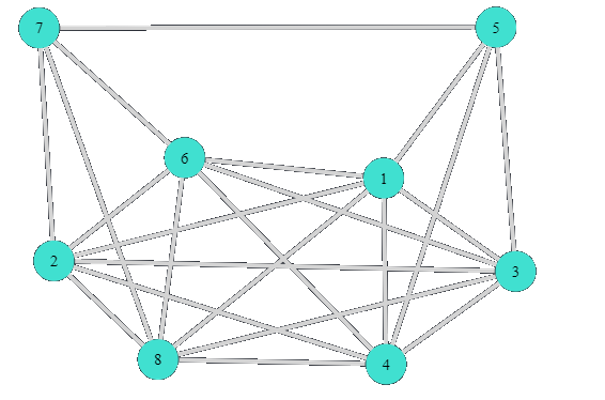
\includegraphics[width=8cm]{Network.png}
%    \caption{Representation of a possible network for eight households}
%    \label{fig:network}
%\end{figure}
\noindent
Note that in this network, not all nodes (which represent households) will be connected to each other, but rather each node will be connected to a selection of different nodes. Based on these connections, households will experience the peer effect. The quantification of the social utility in this setting can be done by using the equation:
\noindent
\begin{equation}
    UT_{soc} = \frac{\#PV}{\#Total}
\end{equation}
Where $\#PV$ is the amount of neighbors a household has that has adopted a PV-battery configuration and $\#Total$ the overall amount of neighbors a certain agent has. The social utility will, therefore, always have a value between 0 and 1. When looking at Figure \ref{fig:network}, the total amount of neighbors can easily be determined by counting the amount of connection that arrive at a certain point. The amount of PV adopters is the central emergent variable in the model and will initially be fuelled by just economic utility, but as adoption increases, so will the social utility and, therefore, the adoption will be fuelled by a mix of economic and social utility.
%\subsubsection{Uncertainty in the ABM}
%Since this model considers investment decisions in DERs, there is going to be a level of uncertainty, since an investment decision will always entail a certain risk. It is, therefore, necessary to introduce some uncertainty in the model. Uncertainty can be incorporated into many aspect of this model:
%\begin{itemize}
%    \item DAM electricity price: By letting the prices vary overtime with some degree %of randomness, uncertainty is introduced into the model.
%    \item Load factor: By letting the load factor fluctuate at random, the production %of the PV becomes uncertain, thereby introducing uncertainty in the model.
%    \item Learning rate technologies: Since the technologies under discussion (PV and %residential batteries) are in a steep growth phase, their prices are still decreasing, but this process still has lots of uncertainty, which could also be used as some form of model uncertainty.
%\end{itemize}
%In this Thesis, the uncertainty in the investment cost is considering the main source of uncertainty. This can be done by considering a set of random projections based on a set of assumptions. Given an average cost decrease ("drift"), there will be a certain random deviation from this path.
\subsubsection{Overall utility}
The overall utility can, finally be computed as:
\begin{equation} \label{totut}
    UT_{tot} = w_{eco}*NUT_{eco} + w_{soc}*UT_{soc}
\end{equation}
With $w_{eco}$ the weighting coefficient for the economic utility and $w_{soc}$ the weighting coefficient for the social utility. Note that these weights are subject to the constraint:
\begin{equation}
    w_{eco} + w_{soc} = 1
\end{equation}
This total utility is to be compared with the adoption threshold of the agent to determine whether the total utility is sufficient to make the household adopt the DERs. These thresholds for different types of households can be found in table \ref{table:threshold}.
\begin{table}[h]
\centering
 \begin{tabular}{||c|c|c||} 
 \hline
 \textbf{Household type} & \textbf{Threshold[-]} & \textbf{Expected payback (years)}\\
 \hline \hline
 Innovators & 0.4 & 16 \\
 Early Adopters &0.5 & 14\\
 Early Majority & 0.6 & 12\\
 Late Majority & 0.7 & 8\\
 Laggards & 0.8 & 6\\
 \hline
 \end{tabular}
 \caption[Overview of the different household thresholds]{Overview of the different household thresholds}
 \label{table:threshold}
\end{table}
\noindent
As mentioned earlier, the utility will mainly consist of economic utility at the beginning of the simulation, when overall adoption is low, but will gradually become a mix of social and economic utility as adoption increases and social utility increases accordingly. It is important to mention that this overall utility is normalised, and will therefore always be between 0 and 1, depending on the weights of the economic and social utility. This is why the thresholds are between 0.4 and 0.8. Note that the values in Table \ref{table:threshold} are estimates since there is no comprehensive literature on the appropriate selection of these values. 
\newline \newline \noindent
Innovators are households that will purchase and install a PV-battery system out of their motivation to adopt new technologies. This motivation will rarely be an economic one, but rather one of social, environmental, cultural or technological standards the household upholds. Their threshold, therefore, is very low, since the innovator does not need any strong economic or social strong incentive to adopt the new technology. Laggards, on the other hand, will not install a new DERs out of any motivation other than a purely utility-based one. Therefore, the overall utility must be high enough to make the laggard adopt the DERs.
\newline 
\newline
\noindent
The question still remains what the distribution is between these different adoption classes. To do so, Rogers' Theory of Innovation Diffusion is used \cite{Rogers}. This theory describes how new technologies or trends get adopted throughout different classes of the population. Note that the terminology used for the different adoption classes (innovators, early adopters, laggards) also comes from this theory. Rogers' research proposes that from a certain population, innovators account for 2.5\% of a population, early adopters for 13.5\%, the early majority 34\%, late majority 34\% and laggards 16\%. %A representation of this distribution for the population in this model can be found in Figure \ref{fig:classes}.
%\begin{figure}[h!]
%    \centering
%    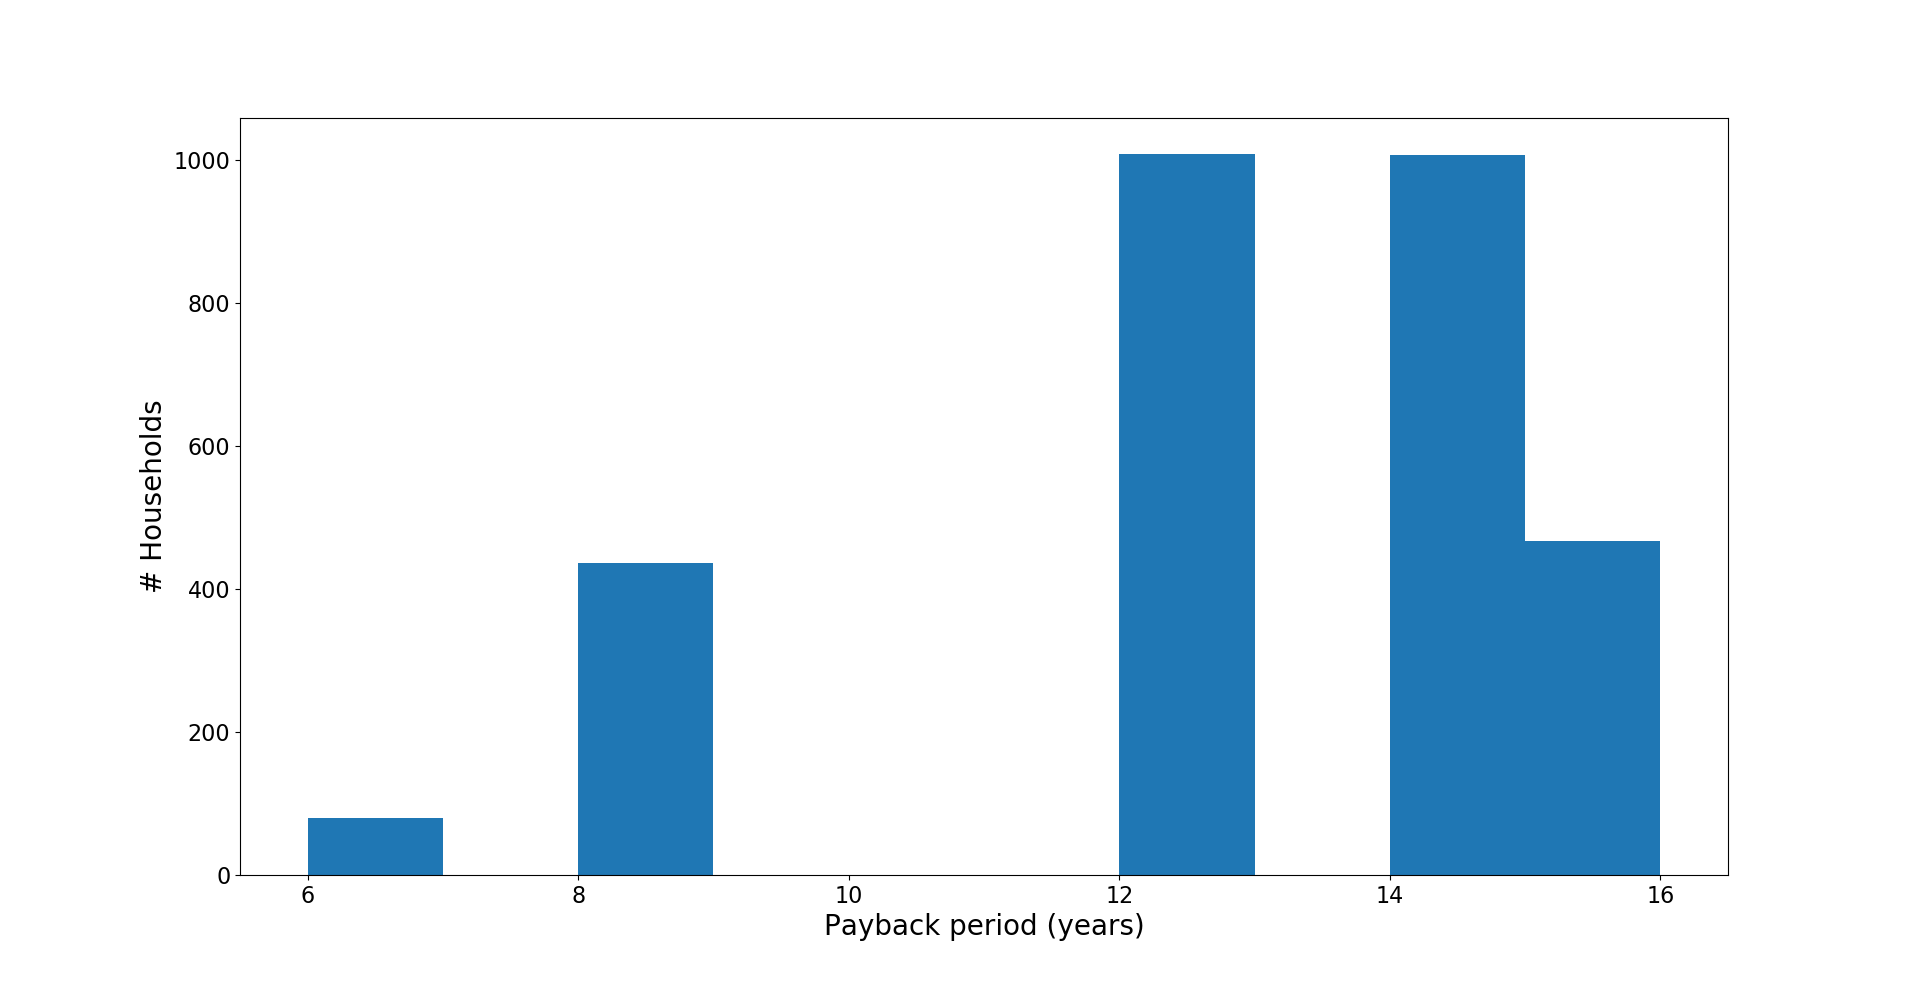
\includegraphics[width=14cm]{Distribution.png}
%    \caption{Distribution of different adoption classes in the model}
%    \label{fig:classes}
%\end{figure}
\chapter{Results \& Discussion}
\section{Introduction}
In this section, the results of the model discussed in Chapter 4 will be presented. In doing so, these results will answer the research question and sub-questions that were formulated in Chapter 1. Since this Thesis attempts to provide qualitative insights into CPT in an ABM framework and is less focused on forecasting a specific case study, the discussion of the results will emphasize on insights into the inner mechanics of the model. With the insights in this model, recommendations can be made with regards to the effect of different policies on the households' DER adoption and utility death spiral. As will become clear from the discussion in the subsequent sections, different policies will have very diverging effects on the adoption rate of PV and battery technologies as well as the network charge evolution. Depending on the goal of policy makers, therefore, different policies can be recommended. In Section \ref{compar}, the different policies will be evaluated by comparing the adoption rates, cumulative capacity, configuration adoption and utility death spiral for each of these policies. Subsequently, in Section \ref{analysis}, some deeper insights in the model shall be provided by analyzing the sensitivity of certain important parameters in the model. These parameters include the loss aversion, residual load and battery subsidy. The effect of the network charge on the model dynamics will also be a point of discussion. In Section \ref{EUTcompar}, the results of the CPT shall be compared with the EUT to discuss the advantages and/or drawbacks of these decision making theories. This chapter will be concluded with Section \ref{future}, where the results will be discussed, concluded and put in the context of broader research and future work.
\newline \newline \noindent
The presented results all come from code implemented in the JuMP environment that is part of Julia 1.1.1 \cite{julia}. The optimization problems were solved using the Gurobi package \cite{julia2}. All plots were generated using the PyPlot extension in the Julia environment.
\section{Policy Comparison}
\label{compar}
The main goals of this Thesis is to determine how different policies influence the adoption of DERs on a residential level. This adoption is to be considered both on a macroscopic level (i.e. what the overall adoption trend is) as well on a more microscopic level (i.e., how the adoption varies between the different configurations discussed in Table \ref{tab:config}). In addition to the adoption of the different configurations, the extent of the utility death spiral (i.e., the evolution of the distribution tariff) will be examined. The policies under evaluation are annual net metering, annual capacity offtake, net billing and battery subsidies (combined with annual net metering). The specifications for each of these policies are:
\begin{itemize}
\item \textbf{Annual net metering}: The prosumer will be able to sell his electricity to the grid at the same rate that he purchased it at. With the intention of decreasing noise in the model as much as possible, the energy price is assumed to be constant at a rate of 0.06 \EUR{}/\textit{kWh} (see Section \ref{development}). The price at which the household will sell his excess electricity will, therefore, also be a constant value of 0.06 \EUR{}/\textit{kWh}. The distribution cost to the prosumer will be determined by means of the net volumetric demand $q_{net}$ and a fixed distribution tariff $dist_{net}$.
\item \textbf{Annual capacity offtake}: Contrary to the previous policy, the annual capacity offtake will charge prosumers according to the peak capacity he will draw from the grid. This peak demand is selected on an annual basis. To make the starting point comparable for both the distribution and capacity tariff, the DSO revenue is assumed to be constant and the same in both cases, since the infrastructure that needs maintenance is the same. Since the DSO revenue for the distribution tariff is calculated as:
\begin{equation} \label{vol}
    Rev = dist_{net}*\sum^{households}_{i=1} q_{net,i}
\end{equation}
		and for the capacity tariff as:
\begin{equation} \label{cap}
    Rev = dist_{cap}*\sum^{households}_{i=1} q_{peak,i}
\end{equation}
Equations \ref{vol} and \ref{cap} can be combined to calculate the capacity tariff:
\begin{equation}
    dist_{cap} = dist_{net}*\frac{\sum^{households}_{i=1} q_{net,i}}{\sum^{ households}_{i=1} q_{peak,i}}
\end{equation}
Which results in a value of 465 \EUR{}/$kWh$. Combining this value with the peak demand of the household $q_{cap}$, the distribution component of the electricity bill can be computed. With regards to the energy component, the prosumer will be compensated and charged equally for the electricity injected into and consumed from the grid. 
\item \textbf{Net billing}: For this policy, the household will get a lower compensation for the electricity he injects into the grid. The tariff that will be used for this policy is a constant value of 0.05 \EUR{}/\textit{kWh}. This difference in tariffs will cause the household to have more incentive to save consumed electricity rather than sell injected electricity onto the grid. This policy will be combined with the net volumetric distribution tariff (similar to that of the annual net metering policy). 
\item \textbf{Battery subsidy}: Contrary to the previously discussed incentives, this policy helps in reducing the investment cost of a DER rather than increasing its operational revenue. This is done in order to encourage the adoption of batteries combined with PV. Since battery adoption has not achieved widespread scalability yet (see Section \ref{Trends}), some subsidies are required to make the technology affordable. In accordance with a recent incentive proposed by the Flemish government, a subsidy of 250 \EUR{} for each \textit{kWh} of residential battery capacity adopted will be introduced into the system \cite{subsidy}. Note that this subsidy is combined with the annual net metering policy in this Thesis. This is done since annual net metering is the most common policy up until now. 
\end{itemize}
These different policies will be evaluated. This will be done by considering the overall adoption, the adoption of the different configurations and the evolution of the network charges to examine the extent of the utility death spiral. 
\subsection{Technology adoption}
\subsubsection{PV}
For the different policies, the overall adoption of PV  technology can be seen in Figure \ref{Figure:PVvolpolicies}. This adoption is given both as a fraction of the entire population and as total capacity adopted. Note that the population consists of 6000 households, 3000 of which have the possibility to adopt DERs, meaning that a 50\% adoption fraction is equivalent to full adoption. The adoption processes of the different policies all follow the S-shaped adoption process like Rogers' innovation theory dictates: the adoption kicks off with a slow adoption (by innovators), followed by a period of steady adoption (when the majority of all actors adopt), only to finish by a saturating adoption by the end of the process, when the laggards will be involved in the adoption process. 
\begin{figure}[h!]
\centering
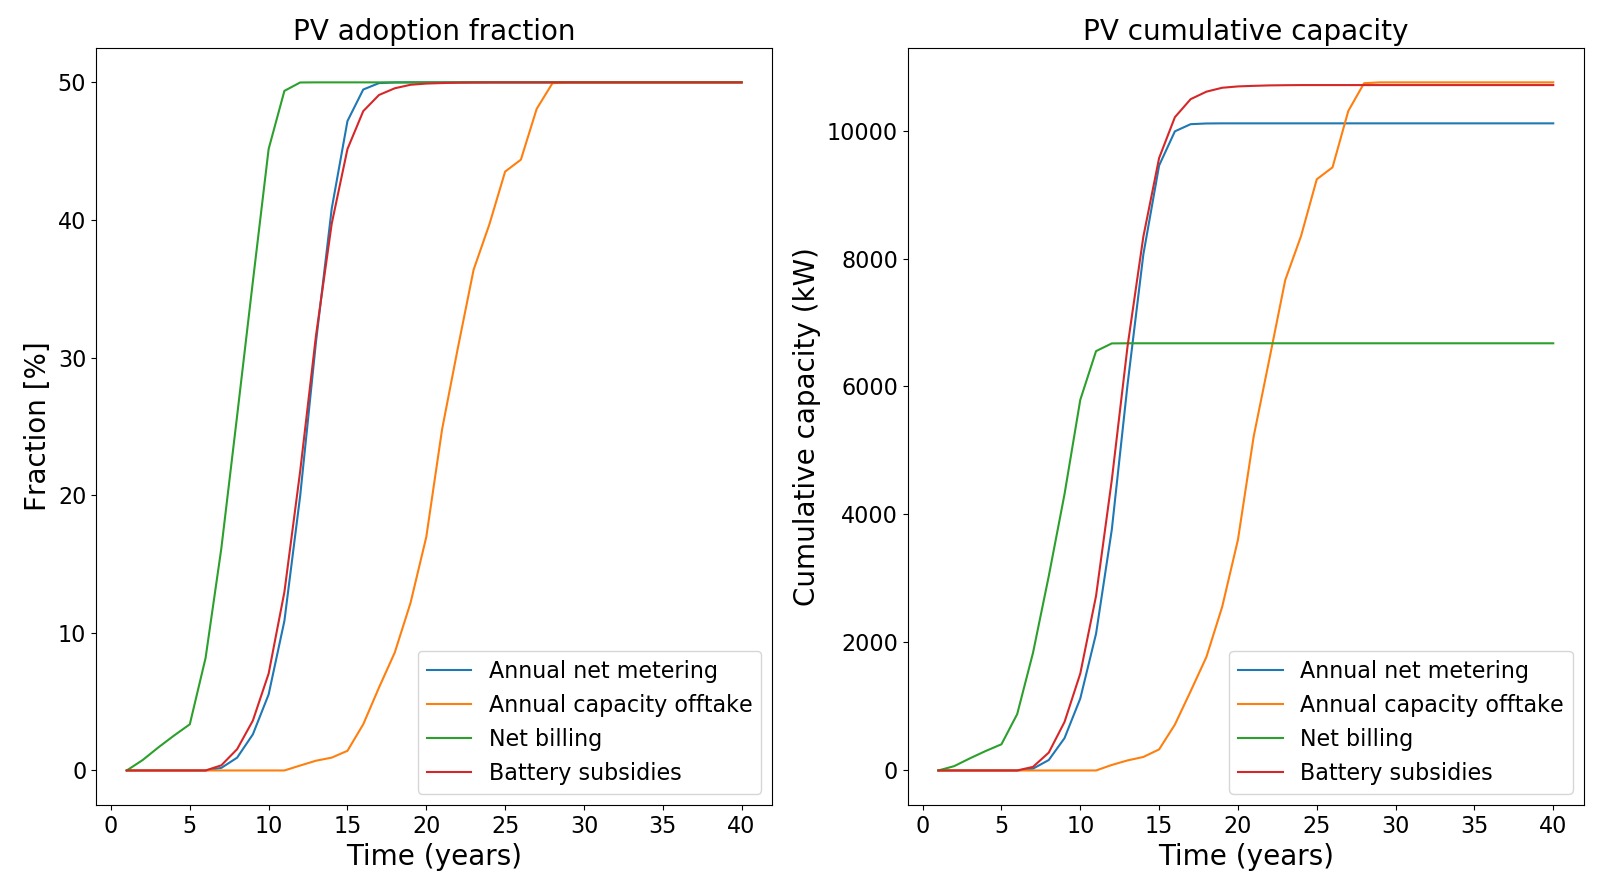
\includegraphics[width=12cm]{Policies/PV.png}
\caption{PV adoption for different policies}
\label{Figure:PVvolpolicies}
\end{figure}
\noindent
The PV adoption kicks off the latest for the capacity offtake tariff. The main reason for this later initiation of the adoption is the lower savings in the case of the capacity offtake tariff (see Section \ref{distanal}). Since the savings realised by the DER are lower, the households will have less incentive to invest. As time goes by, however, the configurations become cheaper. At a certain moment, therefore, the system cost will have sufficiently decreased to make the investment attractive despite the lower savings. Since the adoption in the capacity offtake case occurs almost 10 year later than in the volumetric tariff cases, the technologies are significantly cheaper. This will cause the larger configurations (and large PV panels in particular) to be the preferred option. This is why the overall capacity will be slightly higher for the annual capacity offtake case, even though full adoption is reached more than 15 years later than in the volumetric tariff cases. 
\newline \newline \noindent
The net billing policy will encourage households to become self-sufficient in their energy consumption by adopting DERs. The main reason for this trend in the adoption is the difference between the offtake and injection price of electricity. Since the households must pay 0.06 \EUR{} to consume a \textit{kWh} of electricity from the grid but receives only 0.05 \EUR{} for a \textit{kWh} of electricity injected into the grid, there is an opportunity cost for the household in injecting electricity into the grid. More money can be saved by avoiding electricity consumption than there can be made by injecting the same electricity into the grid. The selection of PV-battery installations will, therefore, mainly happen according to the optimal balance between the investment cost and the electricity savings the installation can bring about. This will make the households more prone to invest in the smaller installations that can supply most of their residential demand without injecting vast amounts of electricity into the grid. 
\newline \newline \noindent
The net metering policy, on the other hand, remunerates the households at the same rate for grid injection as it does for grid offtake. This makes it indifferent to the household whether their PV-battery installation avoids electricity consumption from the grid or whether the PV-battery installation consistently injects electricity into the grid. This will encourage households to install configurations that can maximize the benefits accordingly: the preferred configuration is one that avoids residential consumption while also injecting electricity into the grid. Larger configuration will be more suitable to fulfill this purpose. This will cause the overall adoption PV capacity to be larger for the net metering policy. Since these configurations will be more expensive, their adoption threshold will only be reached after 5 to 6 years, causing the adoption to kick off later for the annual net metering policy compared to net billing.
\newline \newline \noindent
By adding battery subsidies to the net metering policy, the PV adoption shows a similar trend. Although these subsidies do not directly affect the cost of the PV panels, the reduced cost of the batteries will cause the combined cost of several configurations to decrease, thereby making them more attractive to investors. Indirectly, therefore, the battery subsidies will make the PV technology more popular. Note that the overall adopted PV capacity in the case of the battery subsidies will be higher than for the net metering case without battery subsidies (about 5.9\%). At the same time, the adoption fraction for both annual net metering with or without battery subsidies is the same. This is because the battery subsidies will indirectly make larger PV panels in particular more popular. Since larger residential batteries tend to be installed together with larger PV panels (like the 4\textit{kW}/5\textit{kWh}), these configurations will become relatively much cheaper due to the subsidies. This will make the larger PV panels more popular among adopters, causing the average adopted PV size to increase, which results in a higher cumulative PV capacity for the battery subsidy policy. 
\newline \newline \noindent
%\noindent
%\begin{table}[h]
%\centering
 %\begin{tabular}{||c|c|c|C||} 
 %\hline
 %\textbf{Policy} & \textbf{Adopters} & \textbf{Capacity (\textit{kW})} & \textbf{PV
 %/Adopter (\textit{kW})}\\
 %\hline \hline
 %Annual net metering & 3000 & 10,112 & 3.37 \\
 %Annual capacity offtake &3000 & 10,752 & 3.58\\
 %Net billing & 3000 & 6,675 & 2.23\\
% Battery subsidies & 3000 & 10,710 & 3.57\\
% \hline
% \end{tabular}
% \caption[Overview PV adoption data]{Overview PV adoption data}
% \label{table:threshold}
%\end{table}
%\noindent
Due to the difference in incentives between the different policies, the adoption patterns will be different. The annual offtake policy will cause a late kick-off in the adoption but due to the decreased costs, full adoption is reached (i.e. 3000 households) and the cumulative PV capacity even surpasses that of the volumetric tariffs, at a value of 10,752\textit{kW} . This results in a PV capacity of 3.58\textit{kW} per household. Since the smaller, less expensive configurations will be more popular in the net billing case, the adoption threshold for these configurations will be reached quite early in the simulation (year 2-3). The adopted capacity, however, will converge to a value of  6675\textit{kW}. This means that the average adopted PV capacity (among the 3000 households) is 2.23\textit{kW}. Given the fact that the possible PV sizes are 1.5, 2.5 and 4\textit{kW}, the majority of the adopted PV panels will be of the 1.5\textit{kW} kind. For the net metering case, full adoption will also be reached, but this process will be slightly delayed compared to the net billing policy, since the preferred configurations (that can inject significantly into the grid) will only reach the adoption threshold later on in the simulation, mainly due to the cost reduction effects. Compared to the net billing policy, however, the overall adopted capacity will be higher. The final adopted capacity is 10,112 \textit{kW}. Given the fact that 3000 households will adopt PV panels, the average PV capacity installed is 3.37\textit{kW}. Since possible PV configurations are 1.5, 2.5 and 4\textit{kW}, a large amount of 4\textit{kW} panels will be adopted in the annual net metering policy. When subsidies are added to the net metering policy, the aggregate capacity increases to 10,710\textit{kW}. Since the adoption fraction also is 50\% in this policy, 3000 households will adopt PV panels, bringing the average per household to 3.57\textit{kW}. The average PV capacity per household will, therefore, be 5.9\% higher with battery subsidies. A summary of these results can be found in Figure \ref{Figure:pvav}. 
\begin{figure}[h!]
\centering
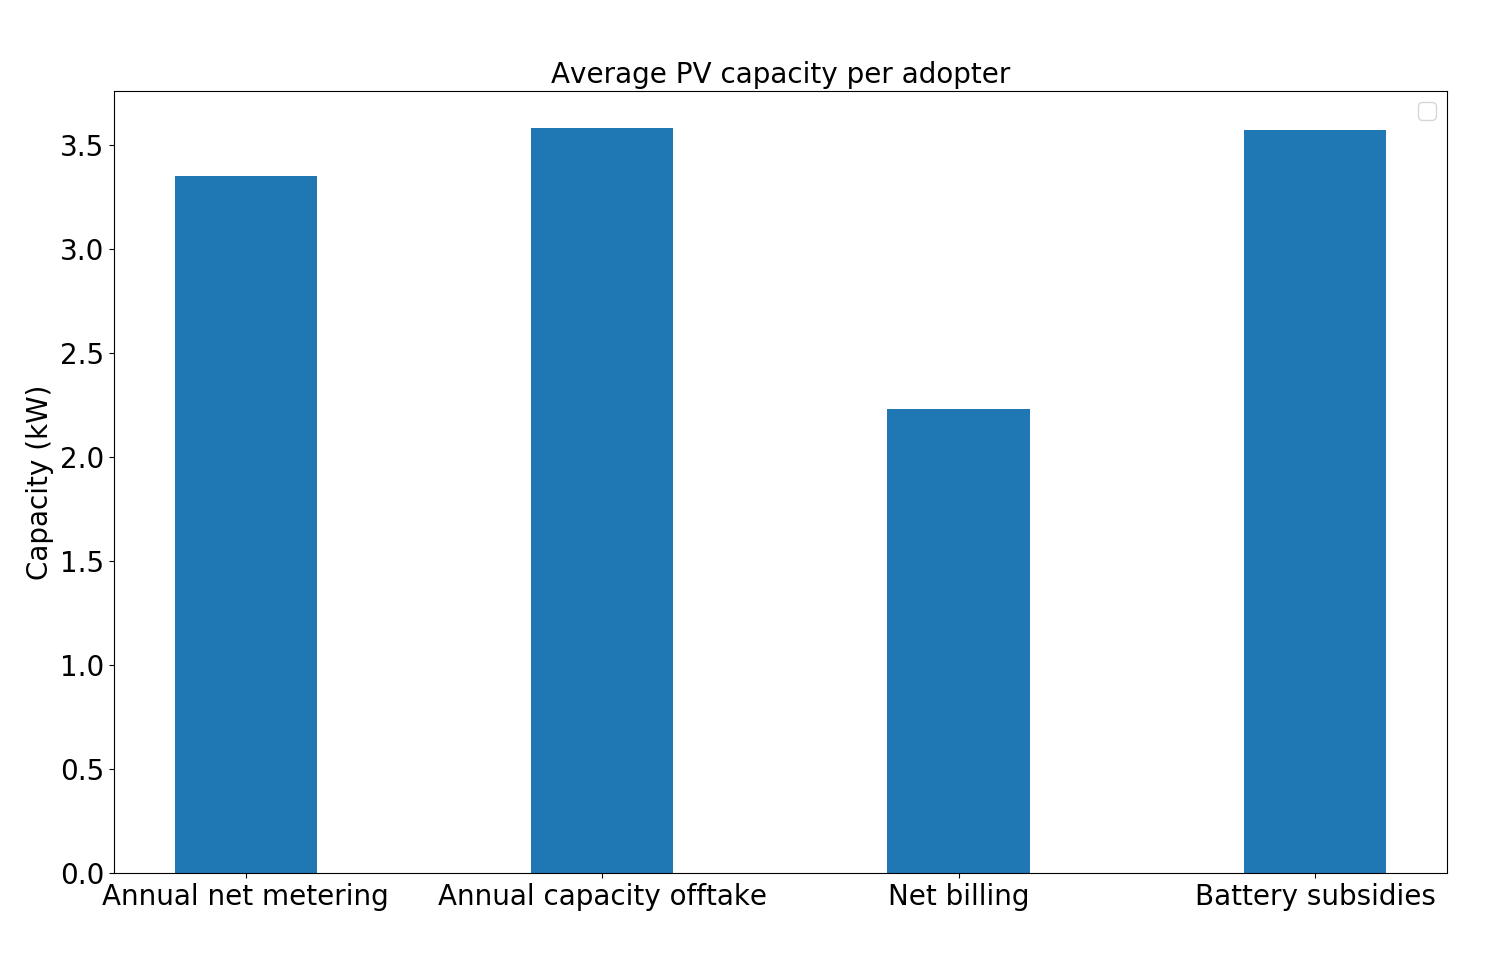
\includegraphics[width=10cm]{Policies/AvPV.png}
\caption{Average PV capacity per household}
\label{Figure:pvav}
\end{figure}
\subsubsection{Batteries}
The battery adoption evolution can be found in Figure \ref{Figure:batpolvol}. The adoption of this technology also follows the S-shaped curve dictated by Rogers' Innovation Theory. Contrary to the PV adoption data, the battery technology adoption is relatively low for the annual capacity offtake tariff. This is due to the difference in costs between PV and batteries: PV panels are a cost competitive technology but batteries still are in heavy development. The latter technology remains expensive compared to the former: note how PV subsidies no longer exist but battery subsidies are a recent government incentive to encourage adoption of this technology \cite{subsidy,Zonnepanelen}. Since the households will realize lower savings under the annual capacity offtake policy, there will be less incentive to invest in expensive batteries. This will cause the cumulative battery adoption capacity to be relatively low compared to the PV adoption levels of the policy.
\newline \newline \noindent
As was the case with the PV adoption data, the battery adoption capacity is relatively low for the net billing case. The battery adoption fraction, however, is also very low compared to the other policies. This is because the preferred configurations are those that save the household the most money due to avoided electricity consumption rather than vast grid injections at minimal investment cost. Since this will cause the total savings the household can realize to be lower, the smaller configurations (i.e. standalone PV panels or panels with a 2\textit{kWh} battery) will be the most popular candidates to fulfill this requirement. Due to these lower savings, the expensive batteries will be less popular among adopters, causing the overall adoption fraction and capacity to be lower. Since the cheaper configurations are the preferred ones, the adoption threshold for these configurations will be reached very early on in the model, causing the net billing adoption process to start the quickest for battery technologies.
\begin{figure}[h!]
\centering
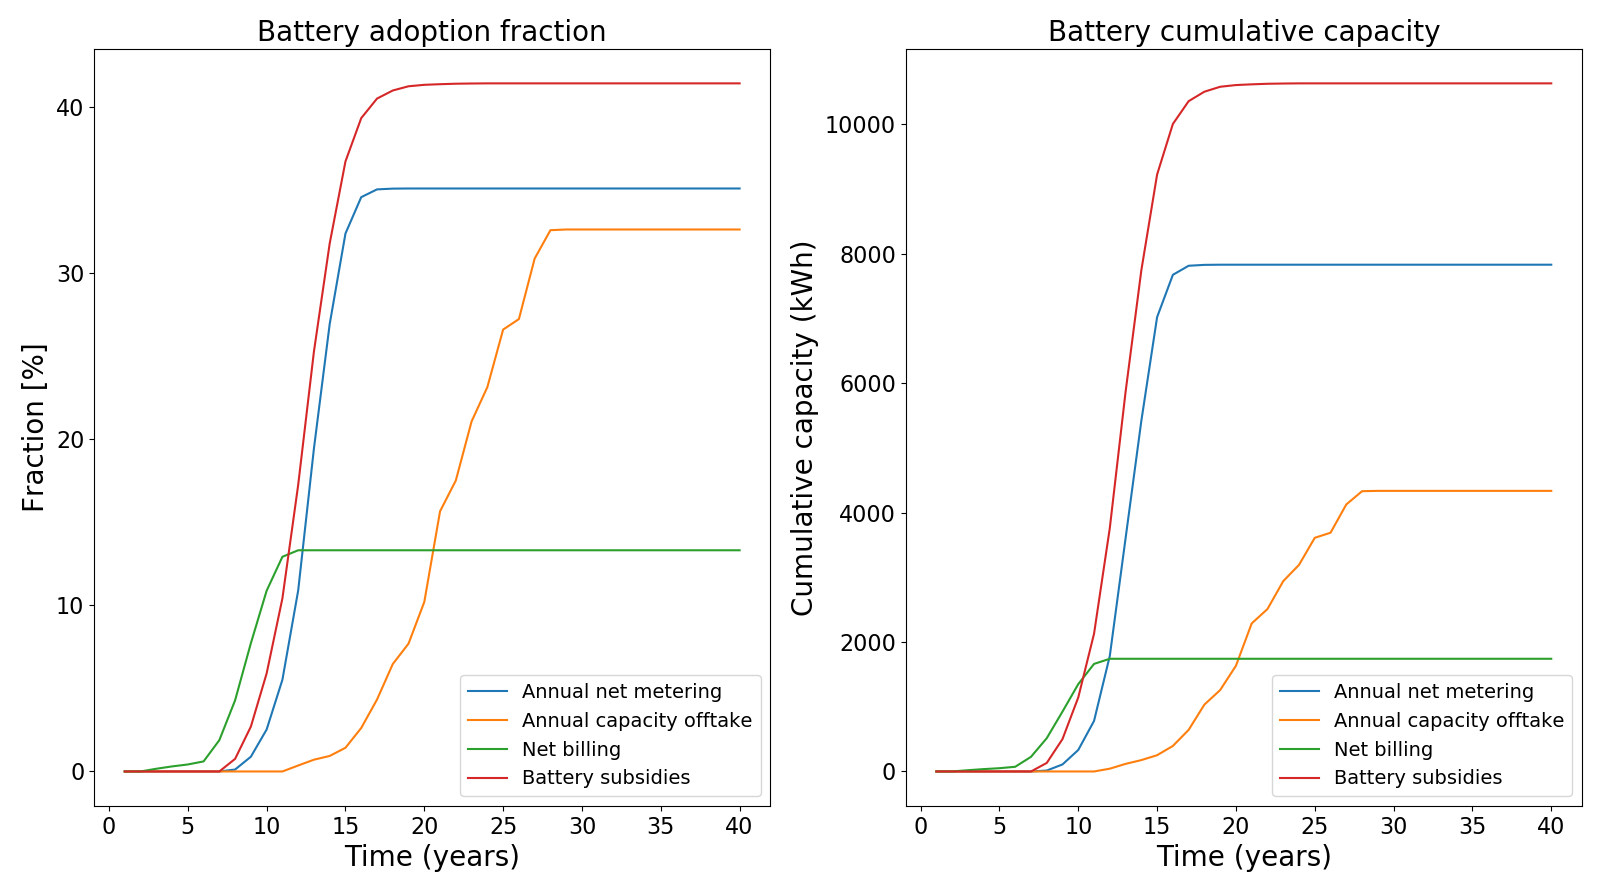
\includegraphics[width=12cm]{Policies/Battery.png}
\caption{Battery adoption for different policies}
\label{Figure:batpolvol}
\end{figure} 
\noindent
For the net metering case, on the other hand, the battery adoption fraction and capacity adopted will be higher than in the net billing case. This is mainly because net metering encourages households to adopt DER for both avoiding grid offtake and increasing grid injection. Larger configurations, therefore, can serve as a means to increase the revenue from continuous grid injection. 
\newline \newline \noindent
The effect of the battery subsidies on the adoption levels is visibly positive. Compared to the net metering case, upon which policy these subsidies are added, the battery subsidy policy shows cumulative adoption capacities that are 35.7\% higher than the case without batteries. Note that the adoption process in the case of the battery subsidies will also happen slightly faster than the case without any financial aid. Battery subsidies will, therefore, incentivize a slightly smaller number of households to adopt larger, more expensive technologies. To accelerate the adoption of large batteries, the battery subsidies can help significantly. When looking into the data of the different policies, the effect of the different policies on the technology adoption becomes even more clear. Since the adoption rate for the annual capacity offtake policy is 32.6\% (i.e. 1956 households) for a cumulative capacity of 4337\textit{kWh}, the average battery capacity per adopter under this policy will be 2.22\textit{kWh}. Since the available options for the batteries are either a 2\textit{kWh} or 5\textit{kWh} module, the average capacity per adopter suggest that the overwhelming majority of adopters will opt for the 2\textit{kWh} alternative.	Since the net billing policy will inherently favor smaller configurations, the average battery capacity per adopter also is smaller: 2.18\textit{kWh}. This is the result of a 13.3\% adoption fraction (which accounts for 798 households) for a cumulative capacity of 1742\textit{kWh}. The annual net metering policy, on the other hand, will make the households prefer larger configurations to increase the benefits of grid injection. Since the adoption fraction is 35.1\% (i.e., 2100 households) and the cumulative capacity is 7832\textit{kWh}, the average battery capacity for each adopter will be 3.73\textit{kWh}, which is significantly higher than the other cases. When considering the available options (2\textit{kWh} \& 5\textit{kWh}), it becomes clear that the average adoption trend has clearly shifted towards the larger alternative. Introducing battery subsidies on top of the annual net metering will cause the overall capacity to increase by 24.7\% to 10,635\textit{kWh} while the adoption fraction will increase from 35.1\% to 41.4\% (2484 households), causing the average battery capacity per adopter to increase by 14.7\% to 4.28\textit{kWh}. This clearly shows how the battery adoption trend will be shifted even more to the larger configurations when battery subsidies are added. A summary of this data can be found in Figure \ref{Figure:batav}.
\begin{figure}[h!]
\centering
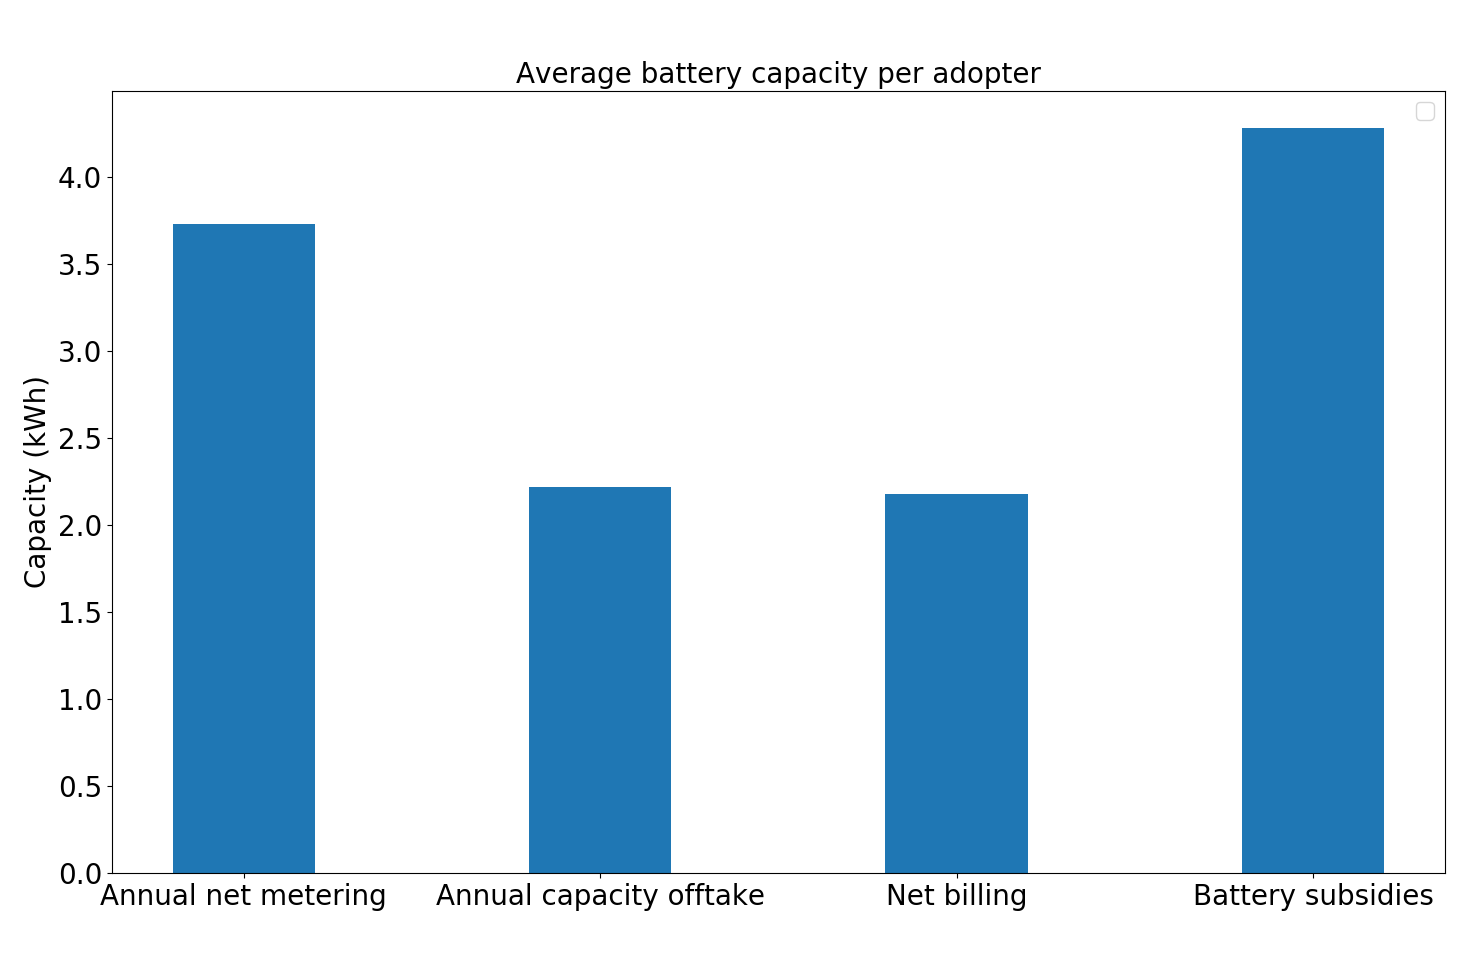
\includegraphics[width=10cm]{Policies/AvBat.png}
\caption{Average battery capacity per household}
\label{Figure:batav}
\end{figure}
\subsection{Configurations}
Besides examining the overall adoption trend, a look into the adoption of the different configurations is also a useful insight into the evaluation of different policies. Figure \ref{Figure:configpol} shows how the different policies drive the popularity of different configurations. Both annual net metering and the same policy combined with battery subsidies favor the larger, more expensive configurations since grid injection can bring substantial benefits to the prosumer. The annual capacity offtake and net billing policy, on the other hand, will make the small and medium-sized configurations more popular. Since the injection tariff is lower than the offtake tariff for the net billing case, self consumption is encouraged and grid injection is discouraged, causing the smaller/less expensive configurations to become more popular.  For the annual capacity offtake case, the combined effects of lower savings and cheaper configurations due to delayed adoption will make the smaller medium-sized installations slightly more popular, with a focus on the larger standalone PV panels (2.5\textit{kW} and 4\textit{kW}) and larger PV panels with a smaller battery (2.5\textit{kW}/2\textit{kWh} and 4\textit{kW}/2\textit{kWh}).  
\begin{figure}[h!]
\centering
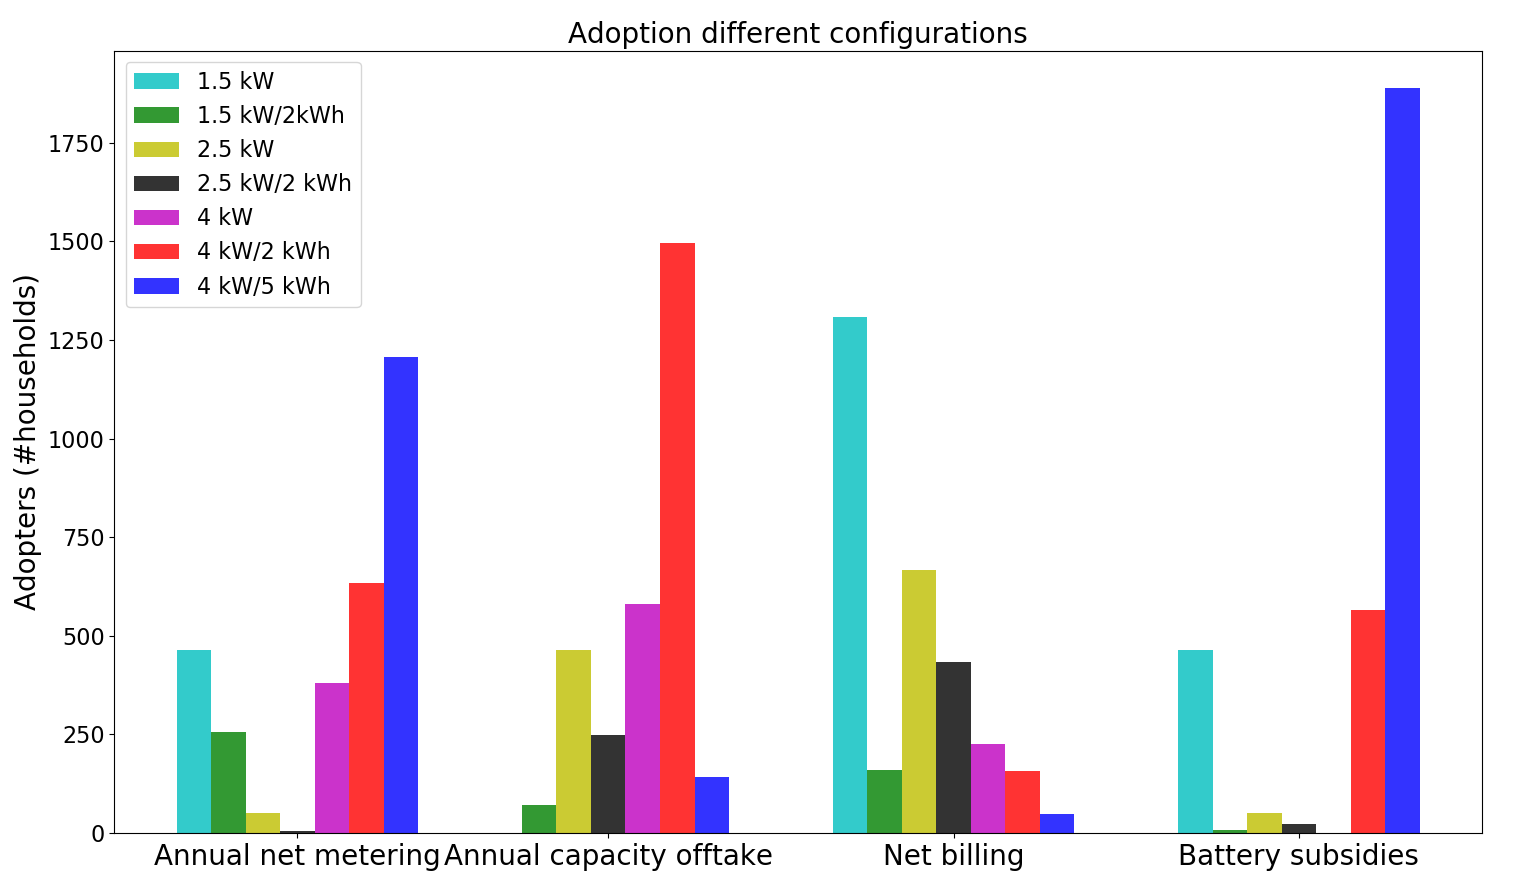
\includegraphics[width=12cm]{Policies/Configurations.png}
\caption{Configurations adoption for different policies}
\label{Figure:configpol}
\end{figure}
\noindent
This adoption data, combined with the adoption processes discussed in the previous section, already gives some insights into the value of different policies to encourage DERs adoption. Policy makers, therefore, should consider these different policies depending to their priorities. 
\newline \newline \noindent
If the goal of the policy makers is to make households adopt PV panels with an optional battery to fulfill their own residential demand, the net billing policy is the most effective. The pricing strategy implied in this renewables scheme will make households adopt PV-battery systems that provide sufficient electricity to supply the majority of the residential demand of the prosumer. The households will be less motivated by the possibility to export excess electricity into the grid. This policy, therefore, implicitly mitigates the widespread injection of residential PVs into the grid, thereby avoiding many grid stability issues.
\newline \newline \noindent
Besides limiting the utility death spiral (see next section), the annual capacity offtake tariff can also help in making the adoption of the different configurations more distributed across the small and medium-sized configurations, with a slight bias toward the standalone 4\textit{kW} and 4\textit{kW}/2\textit{kWh} configuration. The combination of slightly lower savings that the household will be able to realize and the cheaper configurations due to delayed adoption will give him less incentive to adopt the largest configurations (as the net metering and battery subsidy policy do). If policy makers want to change the network charge in the grid while at the same time ensuring a reasonably distributed adoption of different adoptions, the annual capacity offtake policy is a promising candidate. 
\newline \newline \noindent
If, on the other hand, policy makers want to encourage a widespread adoption of larger DER configurations on a residential level to increase the overall produced energy, net metering is the preferred policy. This policy will encourage households to adopt both to supply their residential demand and sell excess electricity to the grid. Although this policy increases the overall adopted DERs capacity and the energy produced by them, it can also bring about grid stability issues. If policy makers want to amplify this effect, battery subsidies can be added to the mix to encourage further adoption of large batteries. 
\subsection{Utility death spiral}
Due to the adoption of the DER on a residential level, the aggregate energy demand of the households will gradually decrease. This will cause the DSO revenue to come under threat, which could make it difficult for the grid operator to maintain and upgrade his infrastructure. As a reaction, the DSO will adapt his pricing towards the end customers. In the case of the annual capacity offtake tariff, the DSO will also need to adapt its pricing since the DER adoption will cause the aggregate peak demand taken from the grid to decrease (a further discussion of these interactions in the model can be found in Section \ref{distanal}). Since the evolution of two different network charges is to be evaluated, the normalised values will be compared. The evolution of these normalised values for the different policies can be seen in Figure \ref{Figure:distpol}. 
\begin{figure}[h!]
\centering
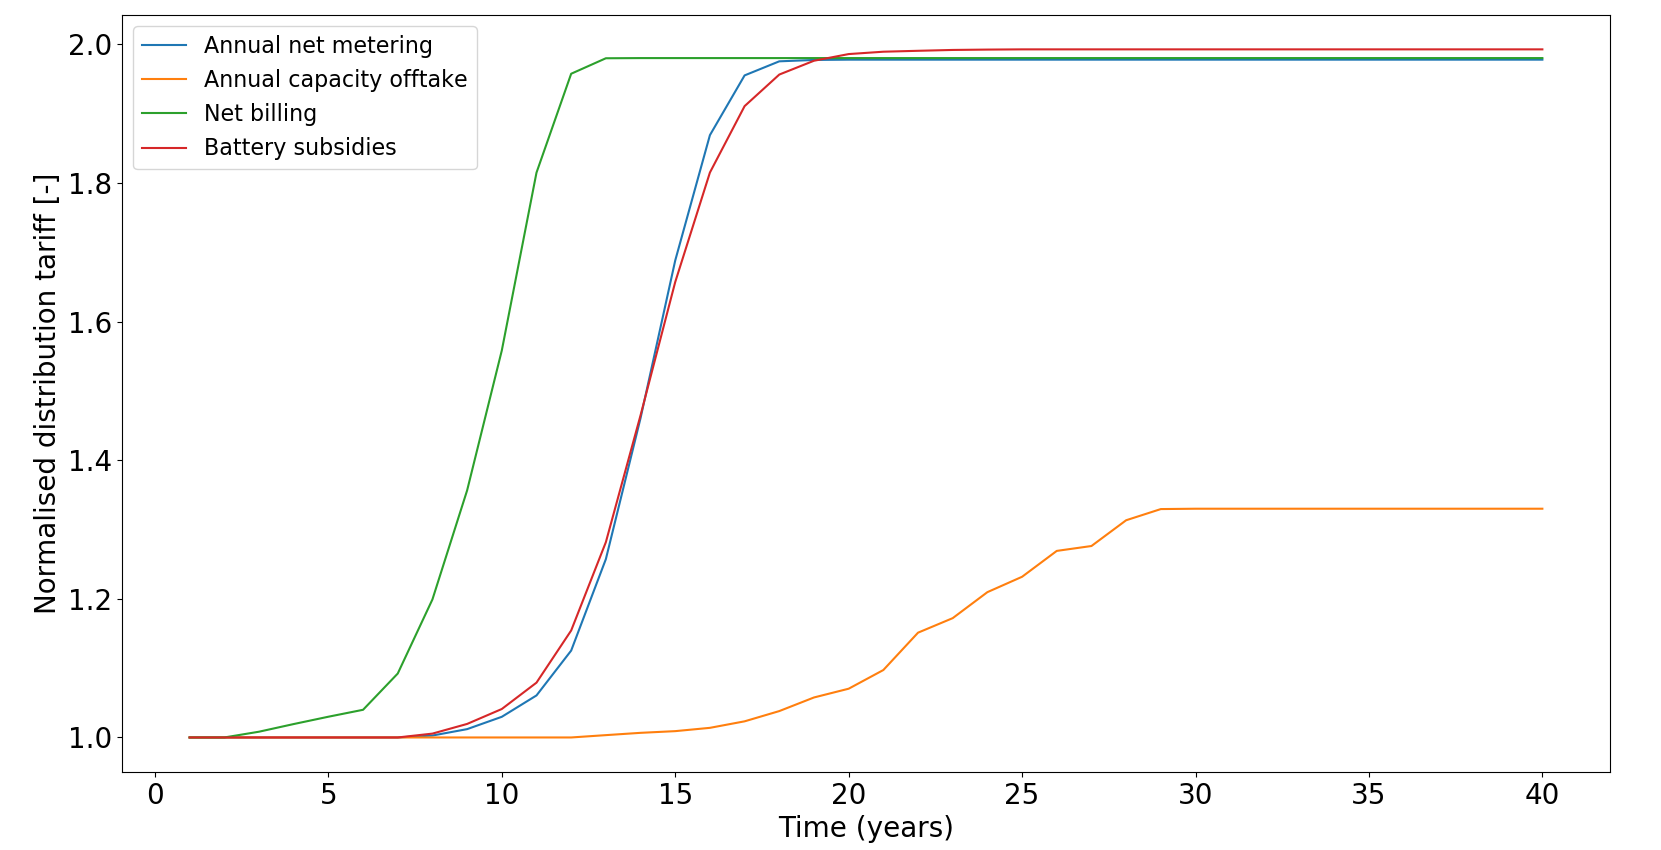
\includegraphics[width=6cm]{Policies/Dist.png}
\caption{Normalized distribution tariff evolution for different policies}
\label{Figure:distpol}
\end{figure}
\noindent
The evolution of the distribution tariff shows a trend that runs in parallel with the DERs adoption: for the quick adoption of the net billing policy, the distribution tariff increases more quickly than for the annual net metering and supplementary battery subsidies case, where DER adoption occurs less quickly. The contrast of the evolution for the volumetric tariff policies with the capacity tariff, however, is the most important trend that can be spotted in this figure. Whereas the distribution tariff increases by  97.8\% in the case of the annual net metering, 98.0\% in the case of net billing and 99.3\% for the battery subsidies case, this increase will only be by 33.0\% in the capacity offtake case. This is a significant difference in tariff evolution. Considering the PV adoption levels for the annual capacity offtake policy, which exceed those of all volumteric tariff-based policies, this limited increase in network charge shows the potential benefits of the annual capacity offtake tariff. 
\newline \newline \noindent
The utility death spiral is, therefore, a phenomenon that will clearly demonstrate itself when a DSO is faced with large DER adoption rates among his customers. Whereas this vicious process will be very clear in the volumetric distribution tariff policies, the capacity offtake tariff will be able to mitigate this effect significantly. 
\subsection{Preliminary analysis \& Conclusion}
The data presented in this section shows how the DER adoption and utility death spiral manifest themselves for different energy-related policies. These results can already lead to certain preliminary conclusions, comparisons and reflections. These will be the main point of discussion for the remainder of this section. 
\newline \newline \noindent
Since the most common policy concerning residential PV is annual net metering, the presented results challenge this choice of policy. Other policies like net billing and the annual capacity offtake show a very different adoption and network charge profile. Among these different alternatives, the efficiency of each one can be evaluated. An adequate DER policy enhances the adoption of these technologies while minimizing the effects/damage to actors other than the households involved or implicated in the adoption process. The most important actor in this aspect is the DSO\footnote{There are many additional actors in this process like the TSO and BSP, but to keep the discussion straightforward, the DSO is a "representation" of the different grid actors}. The important aspects to judge a policy are:
\begin{itemize}
    \item \textbf{Adoption:} The main objective of a DER policy is the diffusion and widespread adoption of PV and battery technology. This adoption should happen quickly (i.e., within an acceptable period of time) and should result in sufficient generation capacity to provide the majority of the residential household electricity demand. 
    \item \textbf{Utility death spiral}: The adoption of the DER should not cause the revenues of the DSO to drop dramatically, since this would make it challenging for the latter to maintain and upgrade his infrastructure, forcing him to adapt the network charges, creating a vicious process that is the utility death spiral. This factor should also be accounted for in the policy choice. 
    \item \textbf{Grid injection \& other}: Although this Thesis mainly focuses on the two aforementioned evaluation parameters, grid injection and the subsequent grid stability issues should also be selection criteria for a policy. Since continuous grid injection by residential DER makes the grid less stable and reliable unless additional reserve and storage capacity is provided, a great deal of costs and headached on behald of the grid operator can be avoided by putting a policy into action that encourages households to adopt DER that limits the amount of grid injection. In the context of this Thesis, the policy must make the households on average prefer smaller configurations over larger configurations.
\end{itemize}
When considering all the available policies (and all possible permutations that could be composed), a few things become clear. The current policy, being annual net metering, scores relatively poorly when considering the evaluation parameters. Although this policy will cause the cumulative adopted DER capacity and subsequent renewable energy produced to be substantial, the adoption process that leads up to this capacity will be relatively slow. For the first evaluation parameter, therefore, the annual net metering will score reasonably well. The next two parameters, however, will perform poorly under this policy: judging by Figure \ref{Figure:distpol}, the utility death spiral effects will be substantial. Since the average adopted DER capacity is large, the grid injection will also be significant. For both criteria, better alternatives have emerged from the results. With regards to the utility death spiral, the annual capacity offtake certainly is the favored candidate (see Figure \ref{Figure:distpol}). By introducing a capacity-based network charge, this vicious circle of DER adoption can be partially avoided. This policy does, however, show the slowest adoption for both PV and battery configurations. The adoption for this policy kicks off ten years later compared to net billing. Judging by Figures \ref{Figure:batpolvol} and \ref{Figure:batav}, the net billing policy will cause the adoption to occur more rapidly. Since the average adopted DER capacity also is lower for this policy, the grid injection will be lower. 
\newline \newline \noindent
The presented results do bear some similarities with previous work in this domain. Previous work attempted to simulate the PV adoption using the EUT. In doing so, many different utility attributes were used, such as advertisement, income and environmental factors \cite{ABMPV,ItalyAdoption}. The adoption results of these studies will be compared to the model developed in this Thesis. The results of the PV adoption by Palmer et al. can be found in Figure \ref{Figure:italyadoption}: 

\begin{figure}[!tbp]
  \centering
  \begin{minipage}[b]{0.4\textwidth}
    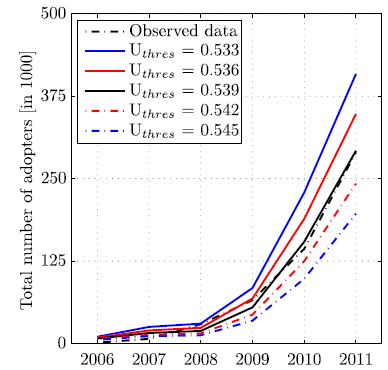
\includegraphics[width=6cm]{Policies/Italyadoption.PNG}
    \caption[PV adoption data Palmer et al.]{PV adoption data Palmer et al. \cite{ItalyAdoption}}
    \label{Figure:italyadoption}
  \end{minipage}
  \hfill
  \begin{minipage}[b]{0.4\textwidth}
    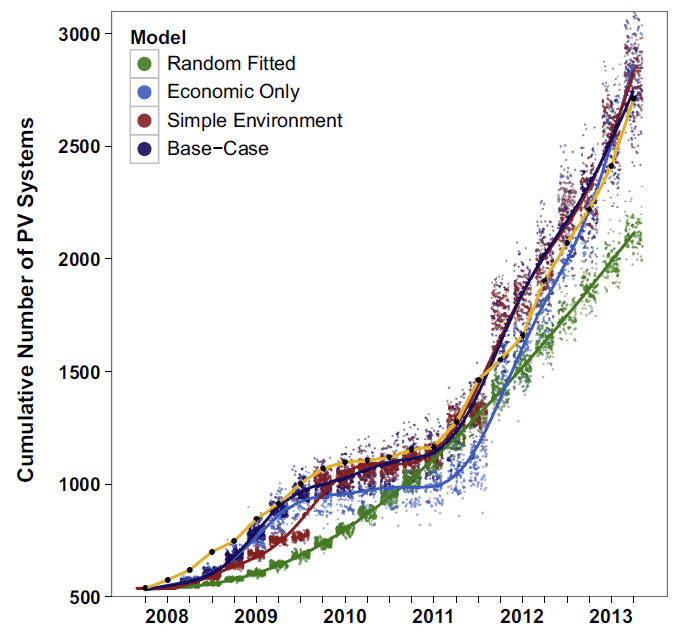
\includegraphics[width=6cm]{Policies/robinsonadoption.PNG}
    \caption[PV adoption data Robinson and Vai]{PV adoption data Robinson and Vai \cite{spatiotemp}}
    \label{Figure:spatiotemp}
  \end{minipage}
\end{figure}
\noindent
In addition, the adoption data obtained by Robinson and Vai can be found in Figure \ref{Figure:spatiotemp}. When comparing this data to the adoption data of this Thesis, as can be seen in Figure \ref{Figure:adopters}, there is a clear similarity with all policies, with the exception of the annual capacity offtake program. All other policies show how the PV adoption kicks off at initially slow rates, followed by a ramp-up in the adoption (which represents an exponential adoption trend). Note how the annual net metering and battery subsidies show the biggest similarity. This data is a good illustration of how new technologies like PV and batteries will emerge. 
\noindent
Note that the time between no adoption and the exponential adoption take between four and five years for both works: For Palmer et al., the adoption starts in 2006 and ramps up exponentially until 2011, while for Robinson and Vai the adoption starts in 2008 and ramps up exponentially until 2013. The data in Figure \ref{Figure:PVcompar} shows a similar trend: for both the annual net metering and battery subsidies, the adoption kicks off in year 6 and has become an exponential by year 10. For the net billing, the adoption kicks off in year 4 and also becomes exponential by year 10. 
\begin{figure}[h!]
\centering
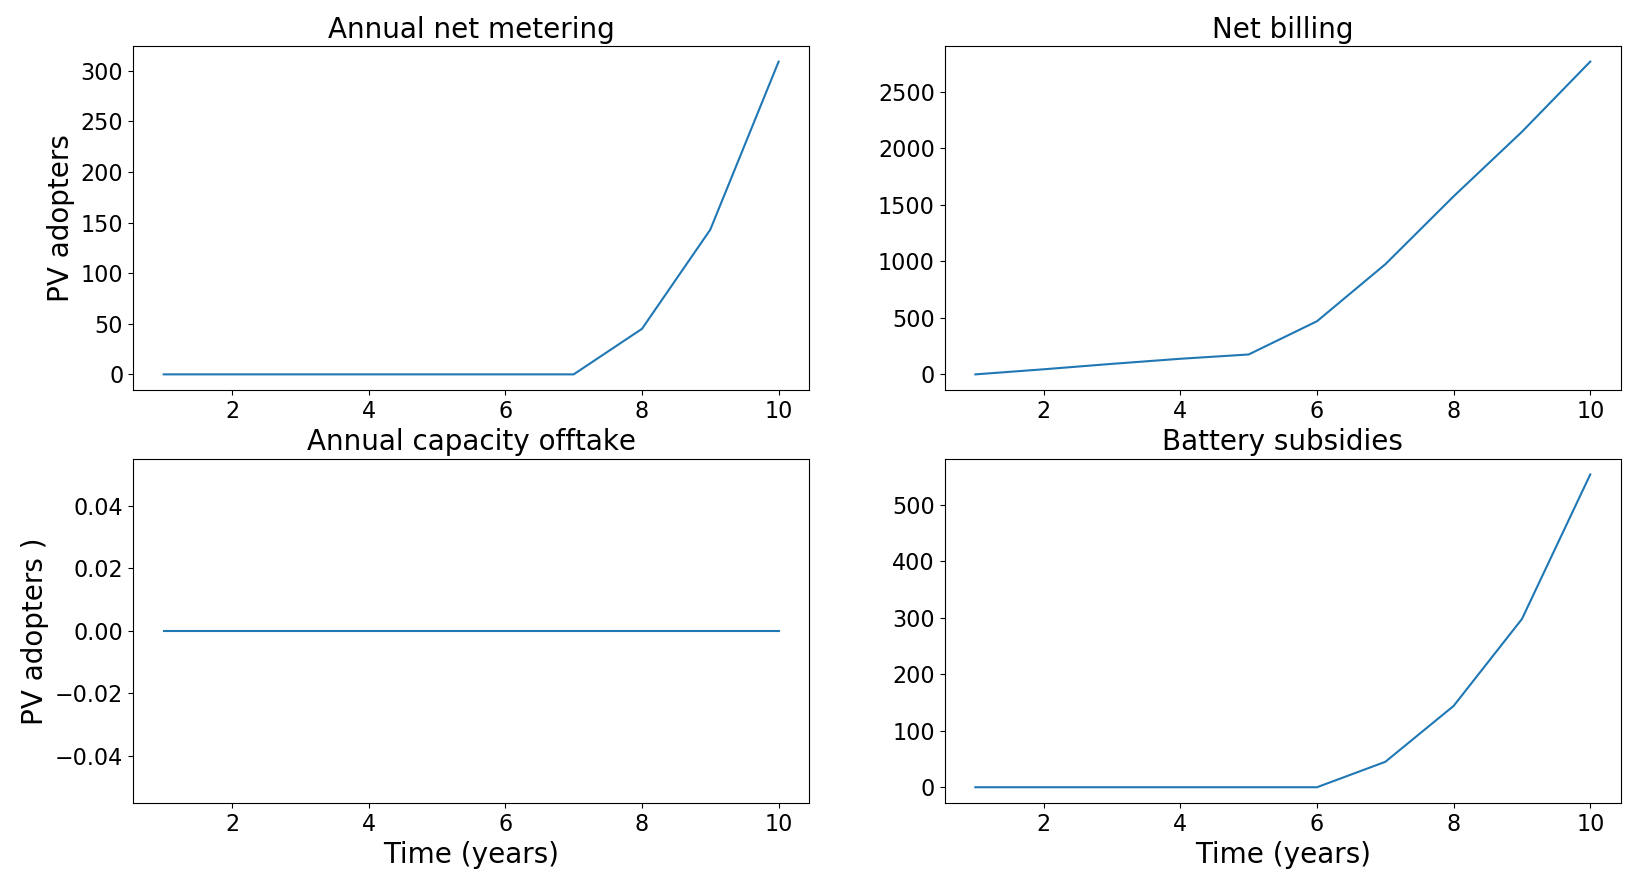
\includegraphics[width=12cm]{Policies/AdoptersCompar.png}
\caption{First ten periods adoption data different polices}
\label{Figure:adopters}
\end{figure}
\noindent
When comparing the data tot that of Zhao et al., as can be seen in Figure \ref{Figure:zhao}, the adoption is considered over a longer period.
%\begin{figure}[h!]
%\centering
%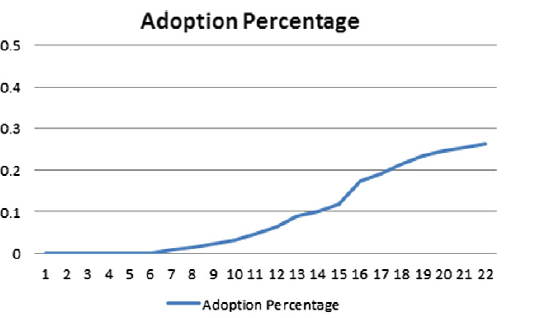
\includegraphics[width=6cm]{Policies/Zhao.PNG}
%\caption[PV adoption Zhao et al.]{PV adoption Zhao et al.  \cite{ABMPV}}
%\label{Figure:zhao}
%\end{figure}
%\noindent
The adoption shows an S-shaped profile, as Rogers' Innovation Theory dictates. This adoption process takes 16 years. When comparing this to the overall adoption data in Figure \ref{Figure:PVvolpolicies}, the PV adoption for the case of net metering starts in year 6 and converges to its final adoption fraction in year 18. The adoption period, therefore, takes 12 years, which slightly lower compared to the adoption period determined by Zhao et al.. Both for the start of the adoption and the entire adoption period, therefore, the results from this Thesis bear many similarities with related works. 
\newline \newline \noindent
The data obtained in this Thesis does, however, show a slightly more uniform trend than the results of the related works. This is due to the lower amount of households considered in this Thesis (3000 vs. 100,000s in other works), causing the heterogeneity of the system to be smaller. This will inevitably cause less values to deviate from the general trend. Since the utility attributes in this Thesis are limited to the welfare and peer effect (since the main purpose was to examine the effects of using CPT in the DER adoption process), the results will behave according to these attributes. The more of these attributes are added, the more complex the behavior of the results will be. Nevertheless, the overall trend of the data obtained in this Thesis is very similar to the one presented in the works by Palmer et al., Robinson and Vai and Zhao et al.. As was discussed in Chapter 3, CPT still faces many challenges before being accepted as an operationalizable model. The main challenge is a general convention for the values of the loss and risk aversion as well as an adequate selection of the reference level to the decision maker. These values, therefore, had to be estimated using both common sense and trial and error in the simulations, since there is no literature available to select generally accepted values. Despite this approach, the results of the model make a lot of sense when comparing them to the Innovation Theory developed by Rogers and the results of other works in this domain of science. 
\newline \newline \noindent
Despite these findings, the results of the model should be treated with a level of scrutiny. Since the utility in this model only considers the welfare and peer effect utility to a certain decision, several aspects of decision making are not accounted for. If the households also incorporate environmental, communication or advertisement effects into their decision making, the decisions influenced by these factors cannot be captured by this model. In addition, the weighting coefficients of Equation \ref{eq:ut} are assumed to be constant throughout the simulation. This gives a level of staticity to the model, despite the intention of this model being to capture the dynamics of the DER adoption process. In next stage, the weighting coefficients should be made endogenous to the model. The author of this Thesis shares this concern with Palmer et al. \cite{ItalyAdoption}. In this work, the authors opted for constant weighting coefficients since they found no mechanism to include this coefficient change into the model. In the setting of this Thesis, however, some recommendation for this change in coefficients can be made. Since the adoption will initially be driven by economic incentives, the economic coefficients should be higher in the beginning of the model. Subsequently, as the adoption increases and the peer effect starts to manifest itself, the economic weighting coefficient of the utility decreases. In parallel, the social weighting coefficient increases. The exact values of this increase and decrease are difficult to postulate and have to be determined by careful analysis and comparison of the model results with actual adoption data. 
\newline \newline \noindent
Another limitation of the model is the strict segregation between the different policies, with the exception of the battery subsidies. From the results discussion, it became clear that every policy has its specific characteristics, like the quick adoption for net billing or higher average capacity for net metering. In reality, however, the potential solution will be a combination of all available options. In a further stage, therefore, different combinations of the policies must be tested to determine the optimal policy combination. 
\section{Model Analysis} \label{analysis}
Given the overall adoption trends, some elements need further discussion. A few key parameters embedded in the model require further analysis. To understand their role in the model, a sensitivity analysis will be performed of these parameters. This sensitivity analysis will be performed for the loss aversion and battery subsidies\footnote{Since the author was constrained by the size of this Thesis, the discussion of the residual load and network charge could not be included in the report but can be found on: }.
\subsection{Loss aversion}
Since this Thesis uses a novel approach of CPT in an ABM to simulate the adoption of DERs, a deeper study into the sensitivity of the parameters governing the prospect value computation is to be performed. The most important variable in prospect theory, besides the prospect value, is the loss aversion parameter $\lambda$. This parameter will indicate how strong the convexity of the loss-facing part of the value function will be (see Figure \ref{Figure:value}). The higher the loss aversion coefficient, therefore, the more negative the prospect value of a negative prospect will be, making the decision maker more willing to take risks to make up for his losses. The inverse is true for a lower value of the loss aversion coefficient. To test this consistency of the model, different values for the loss aversion will be tested to see what effect this has on the model output. Since the value used in this Thesis is $\lambda = 1.5$, variations on this base case can be tested and compared with each other. A first interesting value would be a case where the loss aversion does not amplify the prospect value in the negative domain (i.e., $\lambda = 1$). The second value that will be tested is a loss aversion coefficient larger than the one in the base case, which will be chosen at $\lambda = 2$.  All simulations will be done with the same value for the risk aversion (i.e., $\alpha = \beta = 0.6$). This analysis will be discussed for the net metering policy in this section. The other policies can be found in Appendix \ref{app:2}. 
\newline \newline \noindent
The PV adoption results for the different loss aversion values can be found in Figure \ref{Figure:PVlossvol}: 
\begin{figure}[h!]
\centering
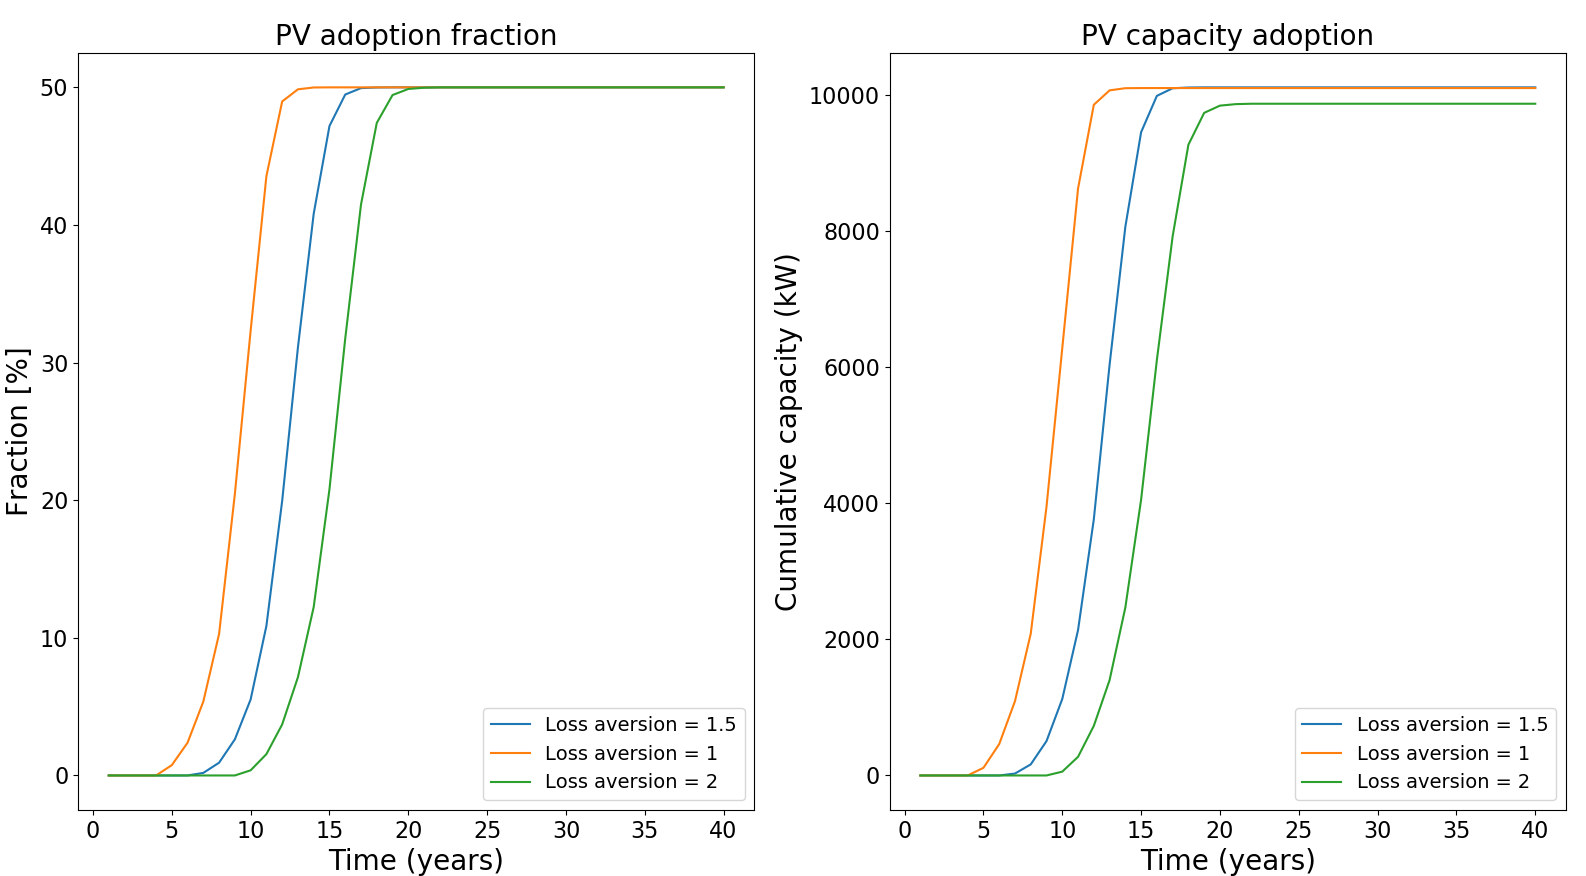
\includegraphics[width=12cm]{ModelAnalysis/PVloss.png}
\caption{PV adoption for different loss aversions}
\label{Figure:PVlossvol}
\end{figure}
\noindent
In this figure, the effect of the loss aversion on the output can be clearly seen: for lower loss aversions, the adoption happens more quickly: whereas in the normal simulation the adoption kicks of in year 7, this already happens in year 4 for the low loss aversion. For the higher loss aversion, the adoption starts later (year 10) and will converge to a slightly lower value. The adoption data for the high loss aversion will show a slightly lower PV capacity than the low loss aversion case. The battery adoption data can be found in Figure \ref{Figure:batlossvol}. 
\begin{figure}[h!]
\centering
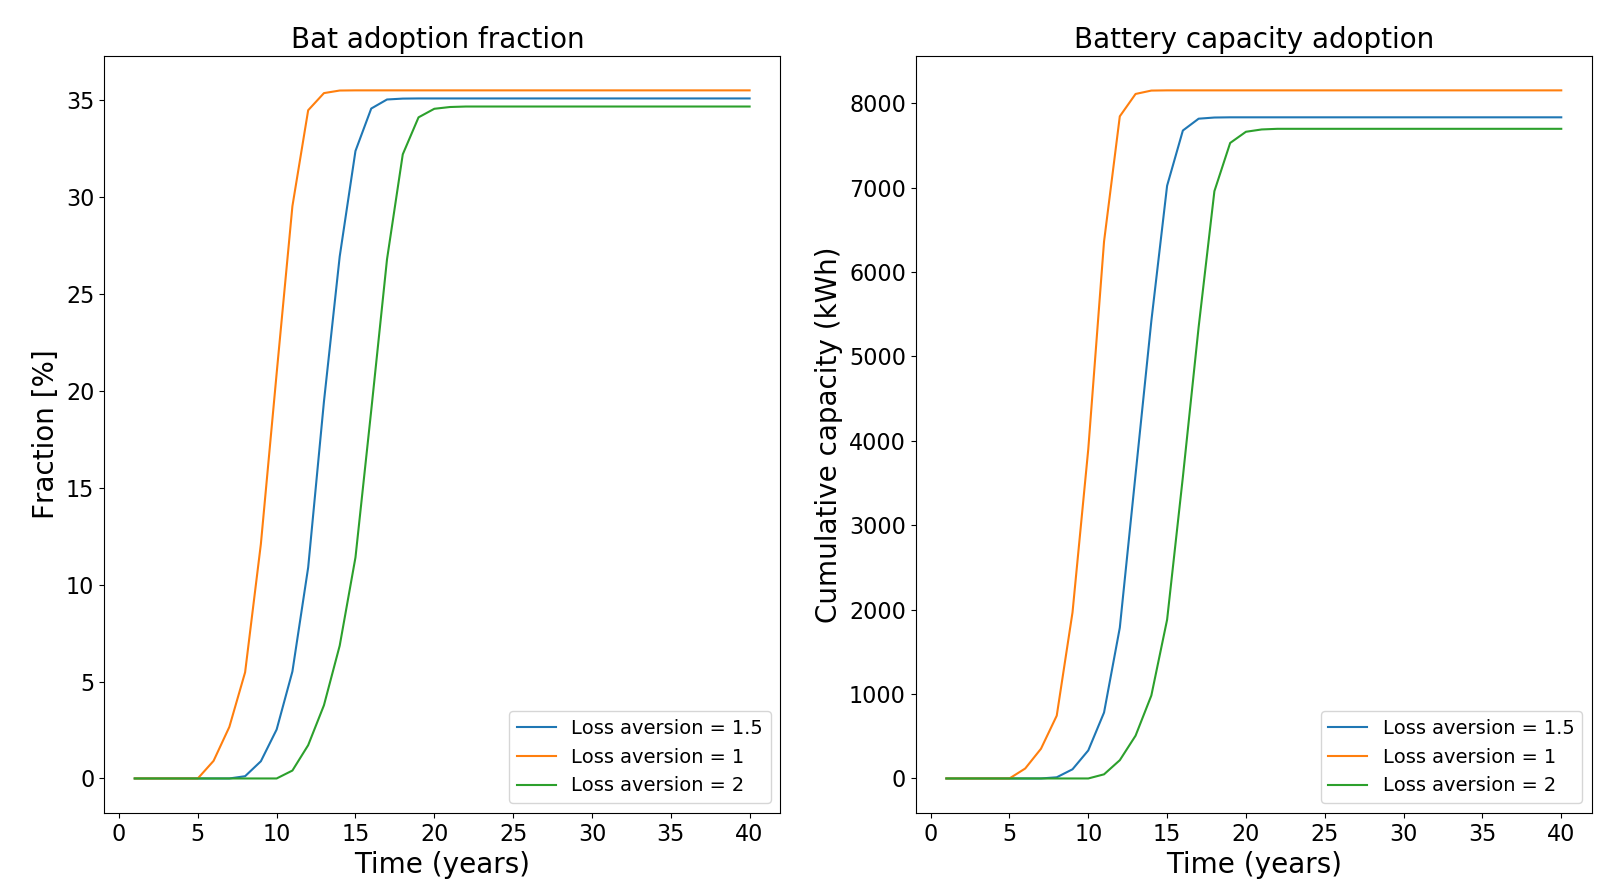
\includegraphics[width=12cm]{ModelAnalysis/Batloss.png}
\caption{Battery adoption for different loss aversions}
\label{Figure:batlossvol}
\end{figure}
\noindent
The battery adoption shows a similar trend as the PV adoption: for the lower loss aversion, the adoption of the technologies happens earlier and to a higher cumulative capacity level. The higher loss aversions will cause the adoption to occur later and at much lower levels. Contrary to the PV data, however, the adoption fraction will also vary as a function of the loss aversion. This analysis shows that the adoption of capital goods like PV panels and batteries are susceptible to a variation in loss aversion. Indeed, when thinking about the connotation of loss aversion, it stands to logic that actors showing high loss aversion will be less likely to invest in these technologies. This effect can be further seen in the configuration distribution, which is presented in Figure \ref{Figure:configlossvol}. 
\begin{figure}[h!]
\centering
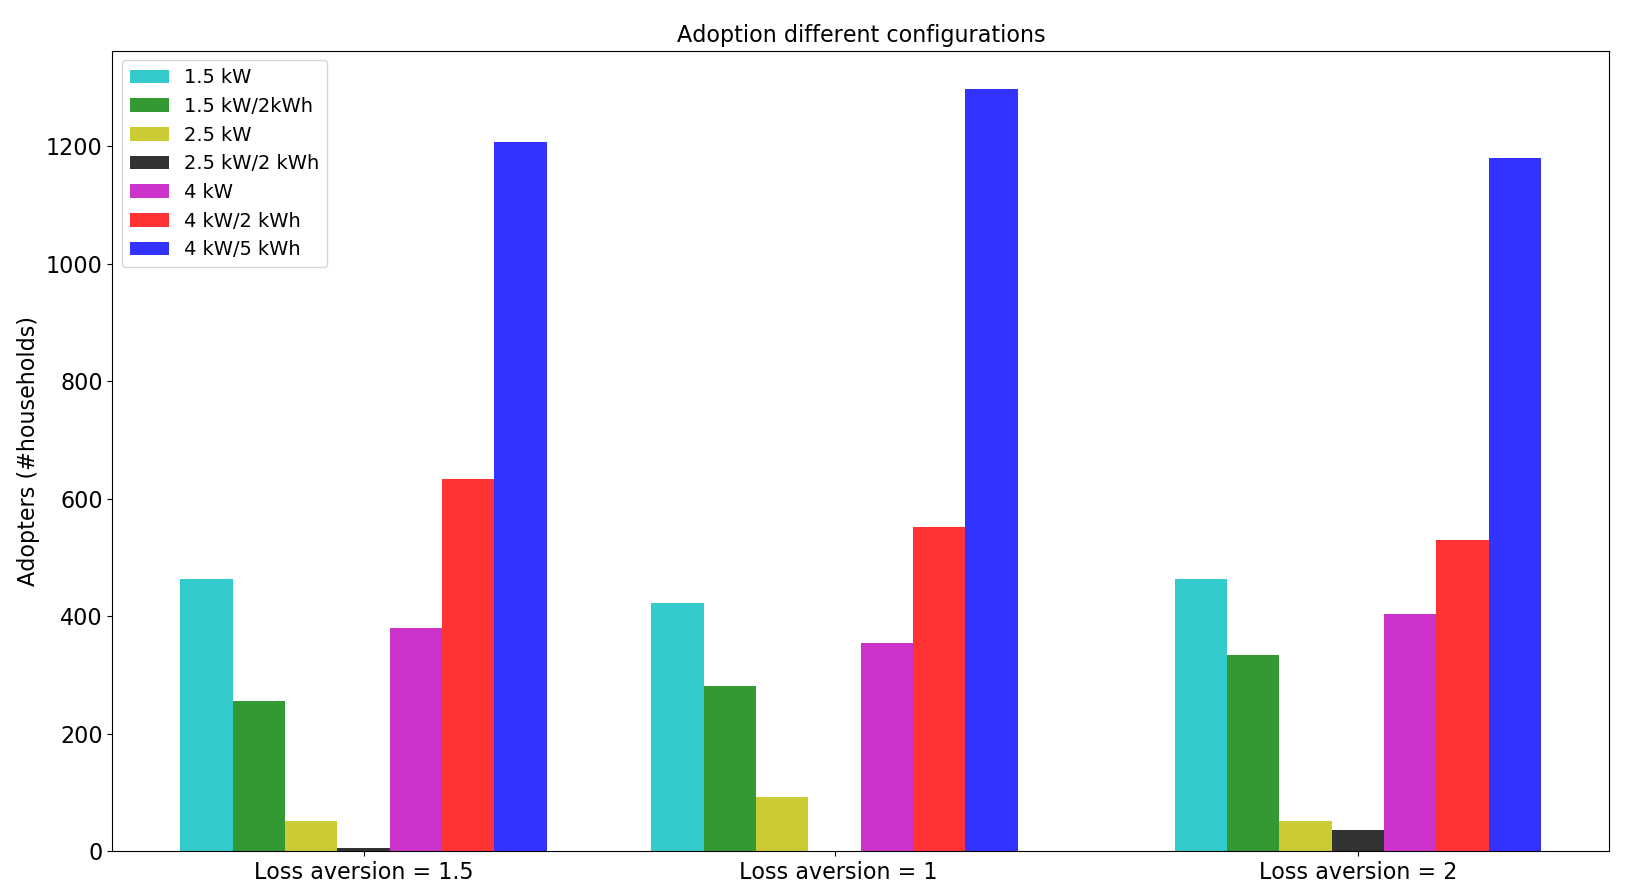
\includegraphics[width=12cm]{ModelAnalysis/Config.png}
\caption{Configurations for different loss aversions}
\label{Figure:configlossvol}
\end{figure}
\noindent
In accordance with the PV and battery adoption rates, the adoption of different configurations shows a slight difference for the different values of the loss aversion. The lower loss aversion values will make the most expensive technology ($4kW/5kWh$) the most popular. Concurrently, the less expensive technologies become less popular. For the higher loss aversion, the opposite will apply: large configurations become less popular whereas small configurations become more popular. The 1.5\textit{kW}/2\textit{kWh} in particular will be more popular for the higher loss aversion. 
\newline \newline \noindent
The utility death spiral that will result from this variation in the loss aversion can be found in Figure \ref{Figure:distlossvol}. Since the adoption happens earlier for the low loss aversion and later for the higher loss aversion, the utility death spiral will manifest itself accordingly.  
\begin{figure}[h!]
\centering
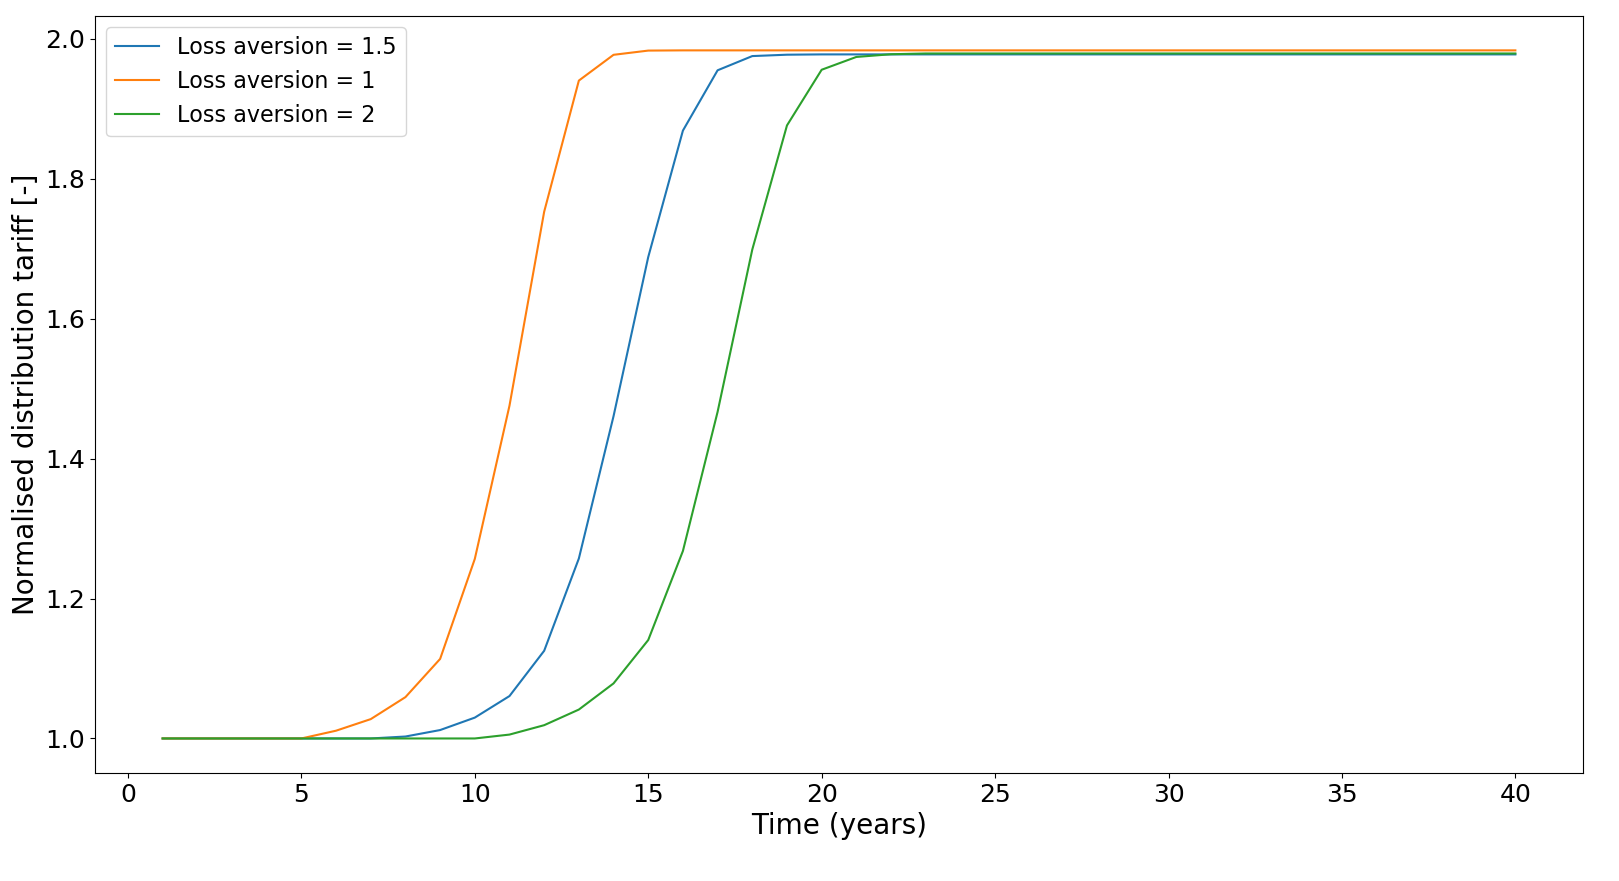
\includegraphics[width=10cm]{ModelAnalysis/Dist.png}
\caption{Distribution cost for different loss aversions}
\label{Figure:distlossvol}
\end{figure}
\noindent
Since CPT is not yet operationalizable as a decision-making theory, performing a sensitivity analysis of the loss aversion is not frequently done. Inversely, obtaining values for the loss and risk aversion will be the ultimate goal of most of the research in this field of research. This analysis, nevertheless, serves as a "stress test" to the model to control whether using the CPT makes sense in this setting. From the results discussion in this setting, there is a clear effect of the loss aversion coefficient on the adoption data. Since these results show a consistent trend for all configurations and technologies, this sensitivity analysis showed how research into CPT as a decision-making theory for simulating DER adoption in a consumer-centric energy system can be add valuable insights. 
%\subsection{Residual load}
%Since the utility death spiral depends on the amount of revenue changes the DSO has to recuperate when a portion of its customers start adopting DER, the residual load of the environment will be the driving force behind this utility death spiral. The higher the residual load as a fraction of the total load, the more recurring revenue the DSO can rely on. This will make it easier for the DSO to pay for all the costs he must incur to maintain and upgrade his infrastructure. A lower residual load, however, will force the DSO to increase his tariffs more to maintain his revenue. The extent of a difference in residual load will be discussed in the subsequent paragraphs. Besides the standard residual load case, where $Resid.\: load = Repl. \:load$, two additional scenarios will be tested. The first one will be for a lower residual load ($Resid. \: load = 0.33*(Repl.\: load)$) and a higher residual load  ($Resid. \: load = 3*(Repl. \: load)$)
%\newline \newline \noindent
%The PV adoption for different residual load cases can be found in Figure \ref{Figure:pvresid}. 
%\begin{figure}[h!]
%\centering
%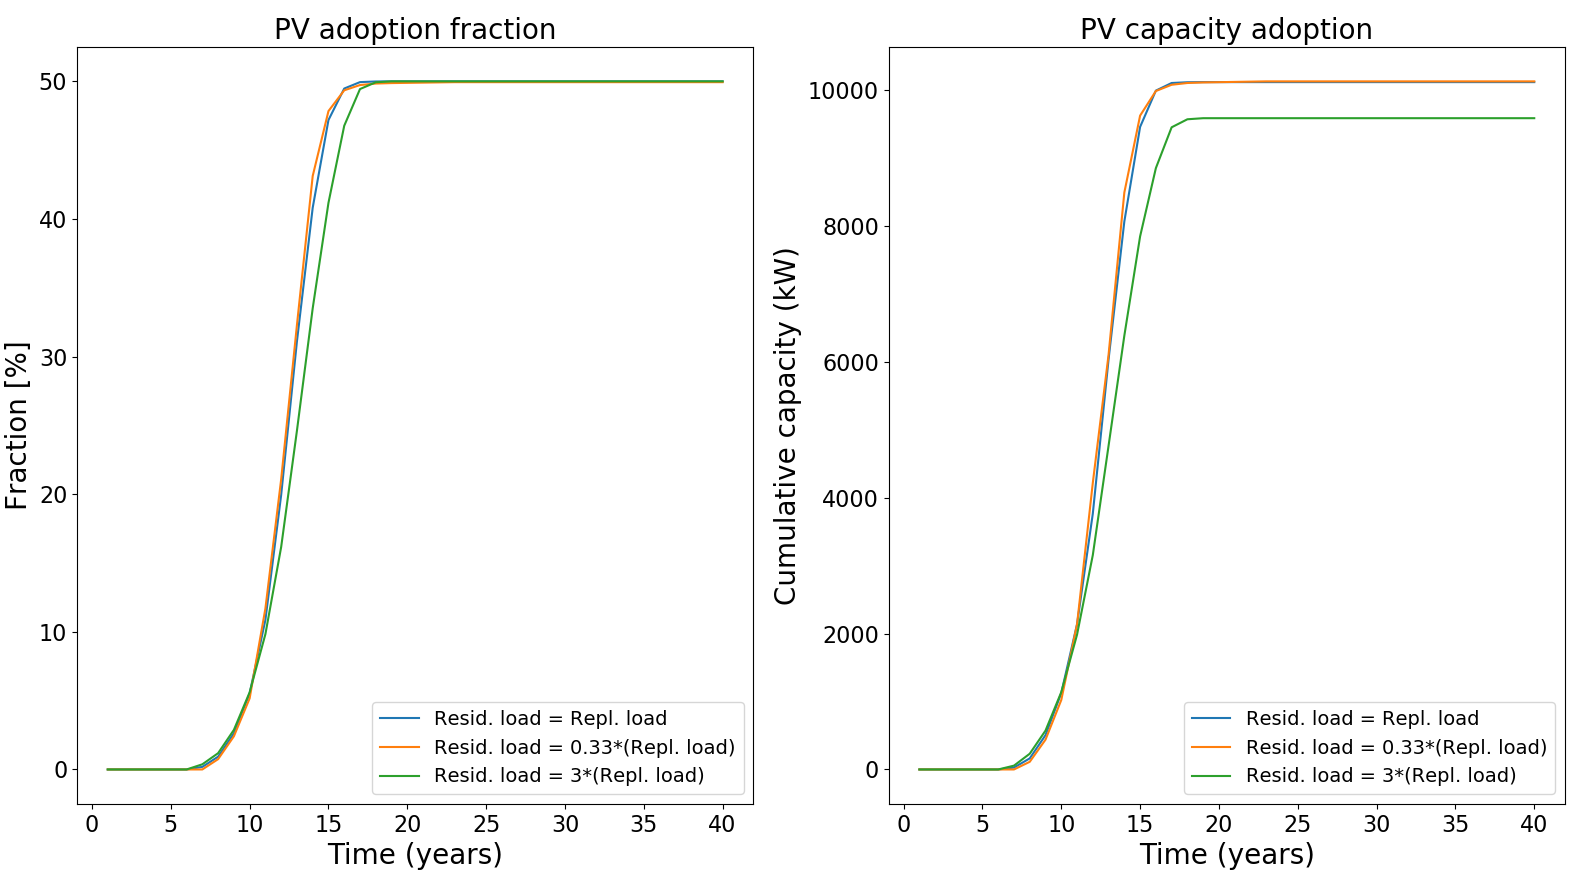
\includegraphics[width=12cm]{ModelAnalysis/PVresid.png}
%\caption{PV adoption for different residual loads}
%\label{Figure:pvresid}
%\end{figure}
% \noindent
%Here, the effect of different residual loads is quite subtle. The results for the three residual loads are quite similar, both in adoption fraction and in cumulative PV capacity adopted. The only exception is the cumulative PV capacity for the higher residual load, which will be slightly lower due to the lower savings. This also applies to the battery technology, although the cumulative capacity does show some more variation, as can be seen in Figure \ref{Figure:batresid}. For both technologies, the cumulative adopted capacity for the higher residual load will be lower since the savings will be lower. These savings will be lower because the DSO will have less recurring revenue to rely on, which will force him to adapt his tariffs more rapidly. For the higher residual load, the opposite effects will play. 
%\begin{figure}[h!]
%\centering
%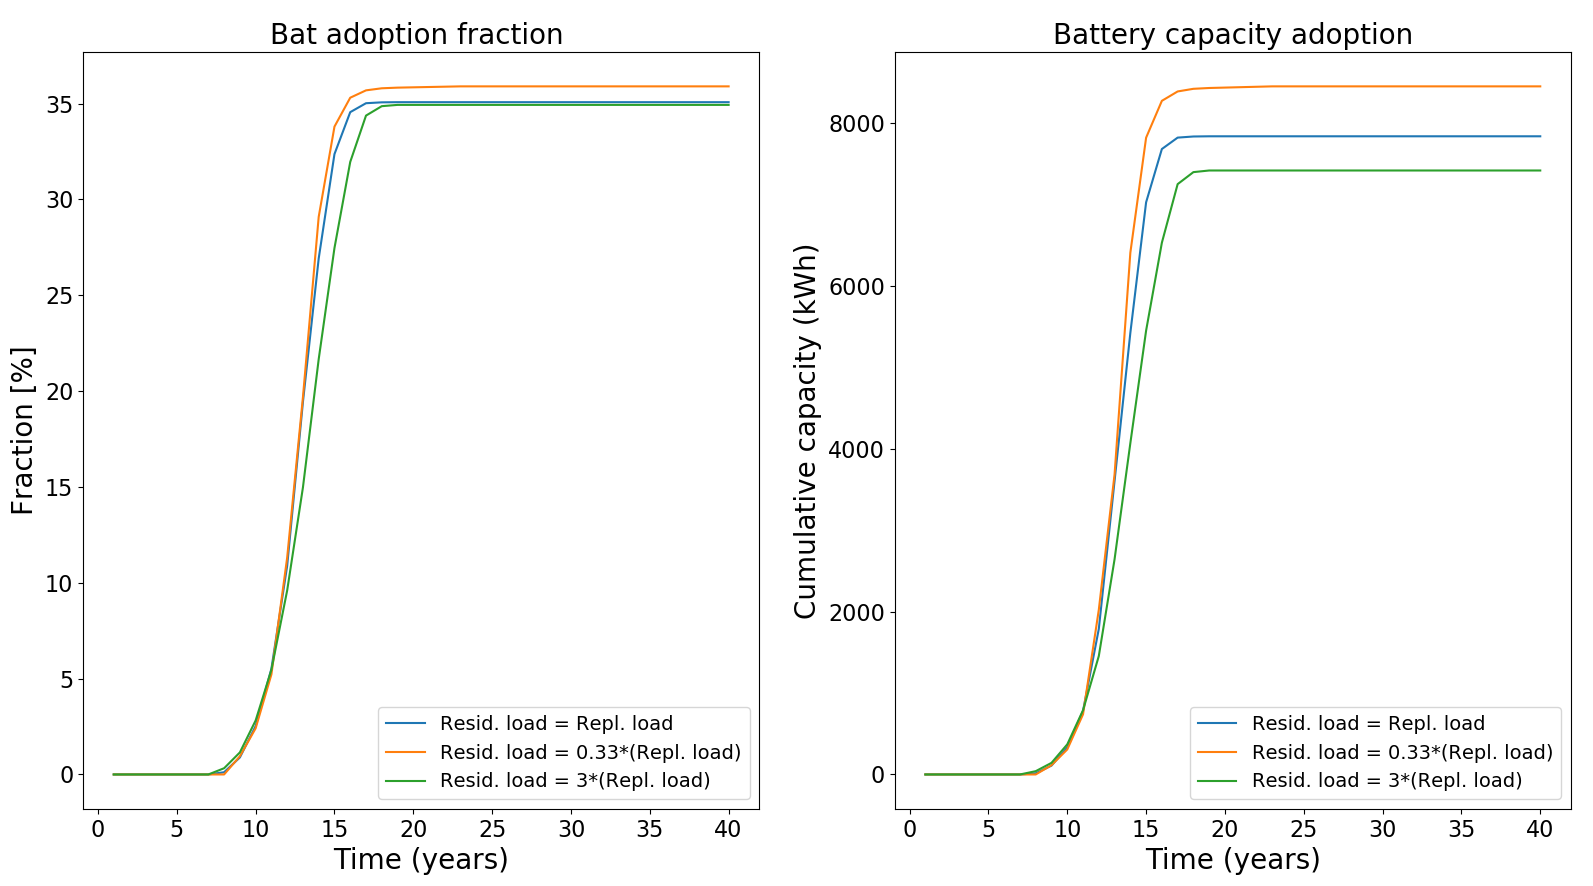
\includegraphics[width=12cm]{ModelAnalysis/BatResid.png}
%\caption{Battery adoption for different residual loads}
%\label{Figure:batresid}
%\end{figure}
 %\noindent
%The resulting configuration distribution can be seen in Figure \ref{Figure:configresid}. Here, the effect of different residual loads becomes more visible. For the lower residual loads, which translates into higher tariffs and savings, the largest configuration (4\textit{kW}/5\textit{kWh}) will become more popular. For the higher residual load, the tariffs and savings will be lower, making this configuration less popular. In fact, the change in battery adoption that can be seen in Figure \ref{Figure:batresid} is mainly due to the variation of this 5\textit{kWh} configuration.
%In addition to the largest configuration, the variation of the residual load will also have an effect on smaller configurations, most notably the 1.5\textit{kW}/2\textit{kWh} installation. Contrary to the larger configurations, this one will become more popular in the high residual load case, when savings are lower, while being less popular in the low residual load case, when savings are higher. The resulting distribution tariff can be found in Figure \ref{Figure:distresid}. In parallel with the adoption levels, the distribution tariff will increase by more than 300\% in the low residual load case, while this increase will only be 33.1\% in the case of a higher residual load. 
%\begin{figure}[h!]
%\centering
%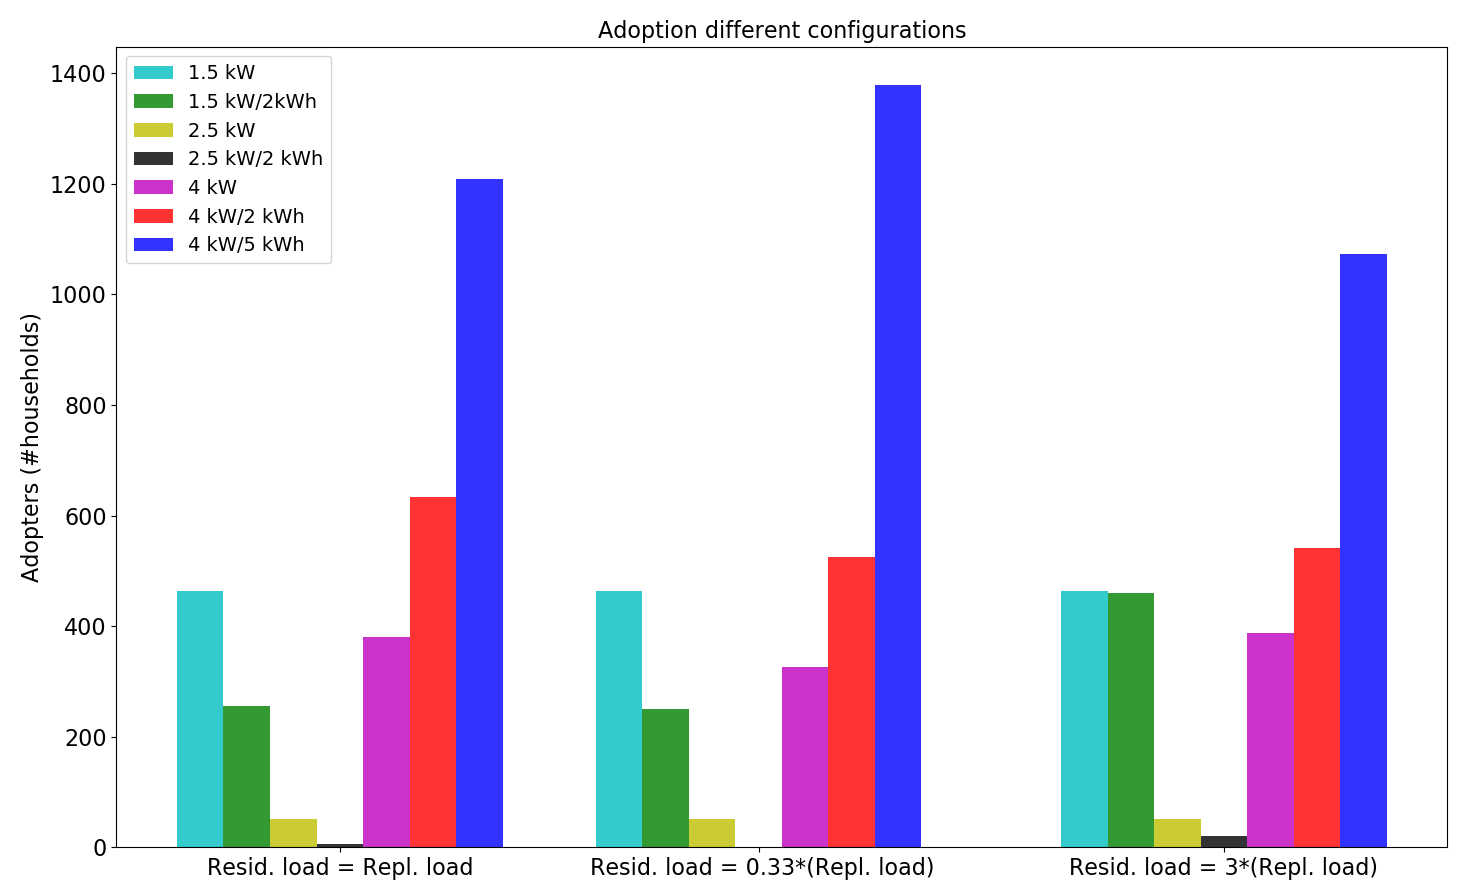
\includegraphics[width=12cm]{ModelAnalysis/ConfigResid.png}
%\caption{Configurations for different residual loads}
%\label{Figure:configresid}
%\end{figure}
% \noindent
 %The resulting configuration distribution can be seen in Figure \ref{Figure:configresid}. Here, the effect of different residual loads becomes more visible. For the lower residual loads, which translates into higher tariffs and savings, the largest configuration (4\textit{kW}/5\textit{kWh}) will become more popular. For the higher residual load, the tariffs and savings will be lower, making this configuration less popular. In fact, the change in battery adoption that can be seen in Figure \ref{Figure:batresid} is mainly due to the variation of this 5\textit{kWh} configuration.
%In addition to the largest configuration, the variation of the residual load will also have an effect on smaller configurations, most notably the 1.5\textit{kW}/2\textit{kWh} installation. Contrary to the larger configurations, this one will become more popular in the high residual load case, when savings are lower, while being less popular in the low residual load case, when savings are higher. The resulting distribution tariff can be found in Figure \ref{Figure:distresid}. In parallel with the adoption levels, the distribution tariff will increase by more than 300\% in the low residual load case, while this increase will only be 33.1\% in the case of a higher residual load. 
%\newline \newline \noindent
%The resulting distribution tariff can be found in Figure \ref{Figure:distresid}. In parallel with the adoption levels, the distribution tariff will increase by more than 300\% in the low residual load case, while this increase will only be 33.1\% in the case of a higher residual load.  
%\begin{figure}[h!]
%\centering
%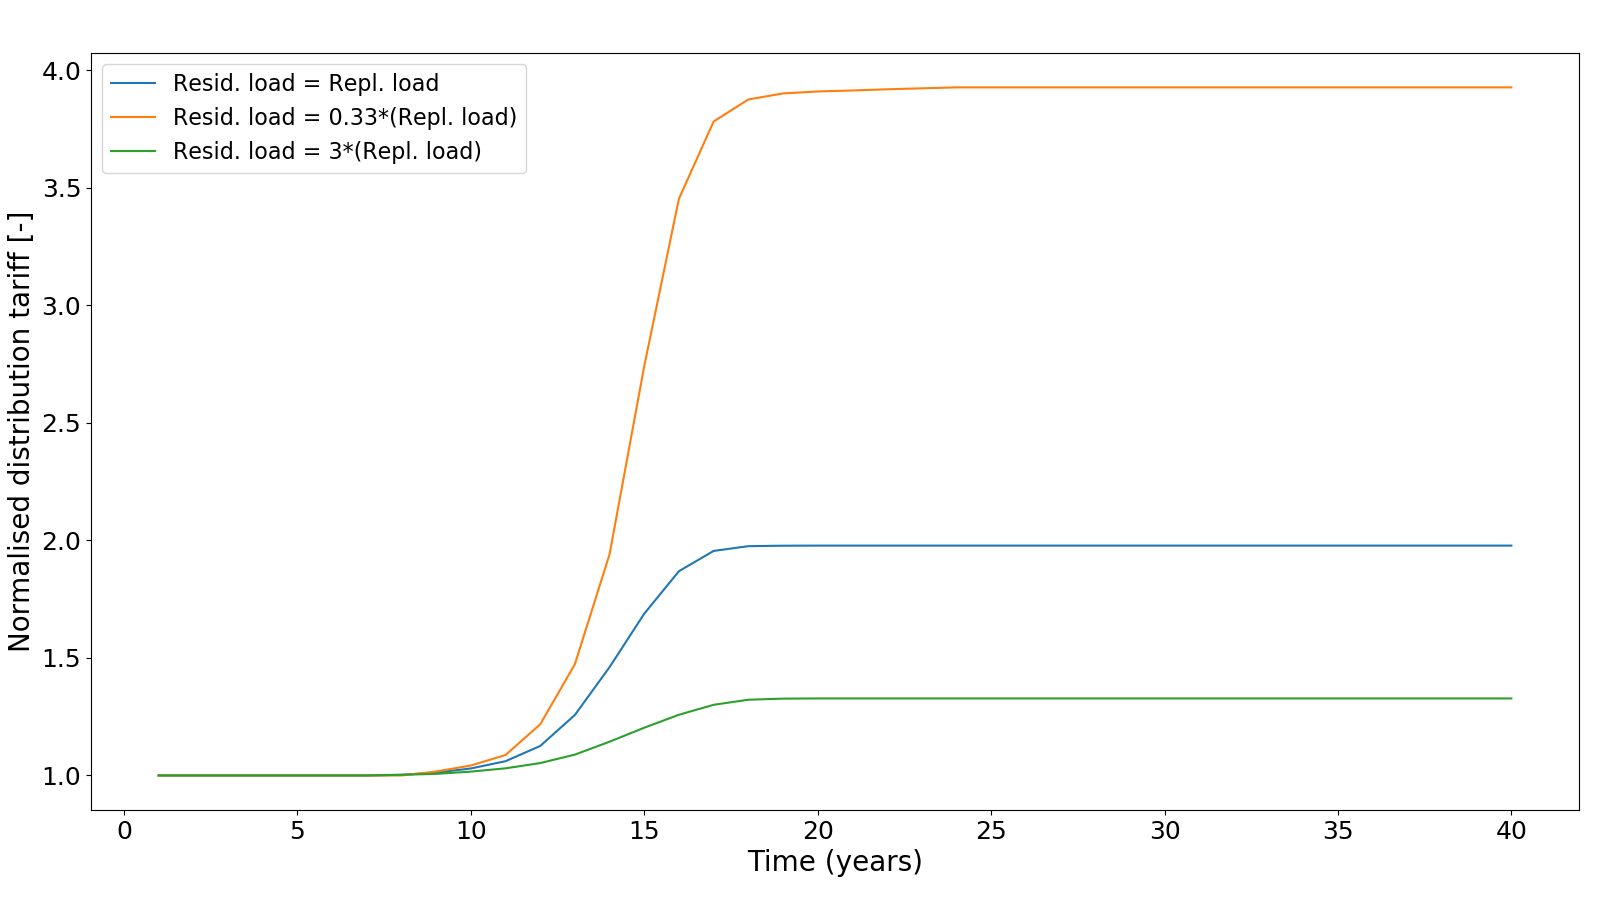
\includegraphics[width=10cm]{ModelAnalysis/distresid.png}
%\caption{Distribution tariff for different residual loads}
%\label{Figure:distresid}
%\end{figure}
%\noindent
%Judging by the data presented in this section, the residual load has an effect on the adoption of certain configurations. Most notably, the adoption of the 1.5\textit{kW}/2\textit{kWh} and 4\textit{kW}/5\textit{kWh} configurations will change as a function of the residual load. This is mainly due to the effect of a change in the network charge on the savings. The lower the residual load, the more popular the large configurations and the less popular the small configurations will be. The higher the residual load, the more popular the smaller configurations are and the less popular the larger configurations. This adoption shift between different configurations will cause the effect on the aggregate adoption fraction and capacity adopted to be rather limited, with the exception of the battery capacity adopted. In parallel with the DER evolution, the network charges will increase in the utility death spiral process. 
\subsection{Battery subsidies}
Since the battery subsidy can decrease the capital requirements for a battery, this incentive could make the technology significantly more popular. An analysis of how different subsidy levels can have an influence on the adoption levels can provide additional insights into this specific policy. Since the policy used in this Thesis is based on the program of the Flemish government for residential battery subsidies, the base case value is 250 \EUR{}/\textit{kWh}. Battery costs, though, are decreasing rapidly and are expected to continue to do so in the future (see Figure \ref{Figure:bloom}). This will most likely cause subsidies to decrease. The different battery subsidy levels that will be tested, therefore, are 150 \EUR{}/\textit{kWh} and 50 \EUR{}/\textit{kWh}.
The PV adoption data for the different subsidies can be found in Figure \ref{Figure:PVsubsvol}:
, \ref{Figure:batsubsvol}, \ref{Figure:configsubsvol} and \ref{Figure:distsubvol}. 
\begin{figure}[h!]
\centering
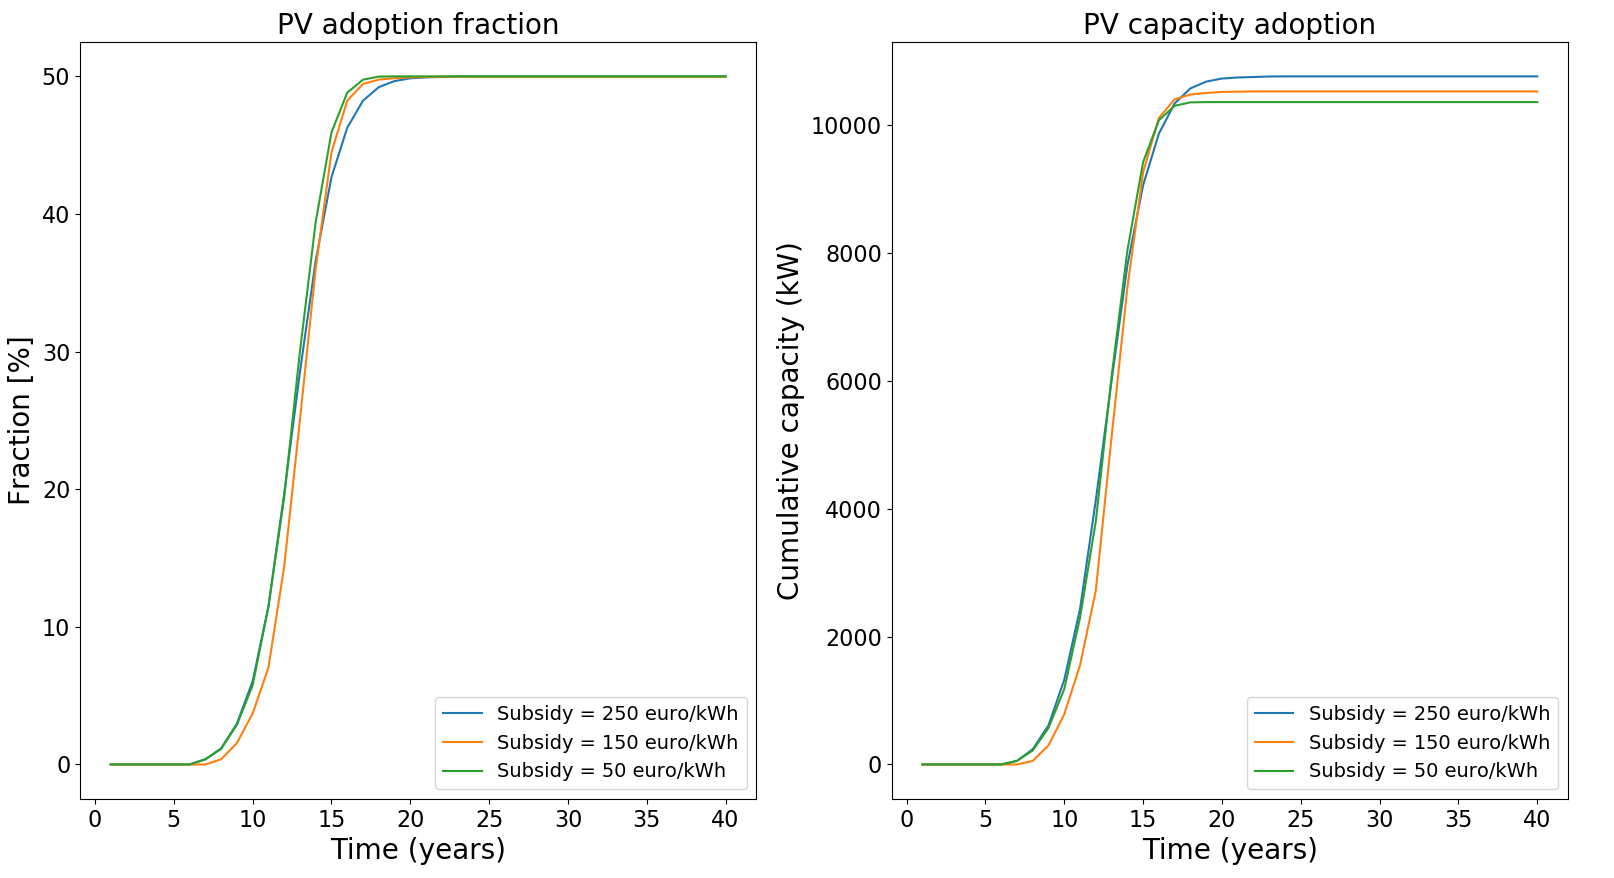
\includegraphics[width=12cm]{ModelAnalysis/PVsubs.png}
\caption{PV adoption for different battery subsidies}
\label{Figure:PVsubsvol}
\end{figure}
 \noindent 
Interestingly, the higher subsidies do not show a visibly higher adoption of PV adopters or capacity. Since higher battery subsidies make the capital costs and payback period of several configurations lower, this should make the adoption incentive for PV-battery systems and PV panels themselves higher. The data in Figure \ref{Figure:PVsubsvol},  however, shows that the difference between the different policies is small. As will become clear from Figure \ref{Figure:configsubsvol}, this is mainly due to a shift in preferences among the three different 4\textit{kW} configurations, which will cause the overall adopted PV capacity to change very little. Between the highest and lowest subsidy, the difference in PV capacity adopted is 3.9\% . 
\begin{figure}[h!]
\centering
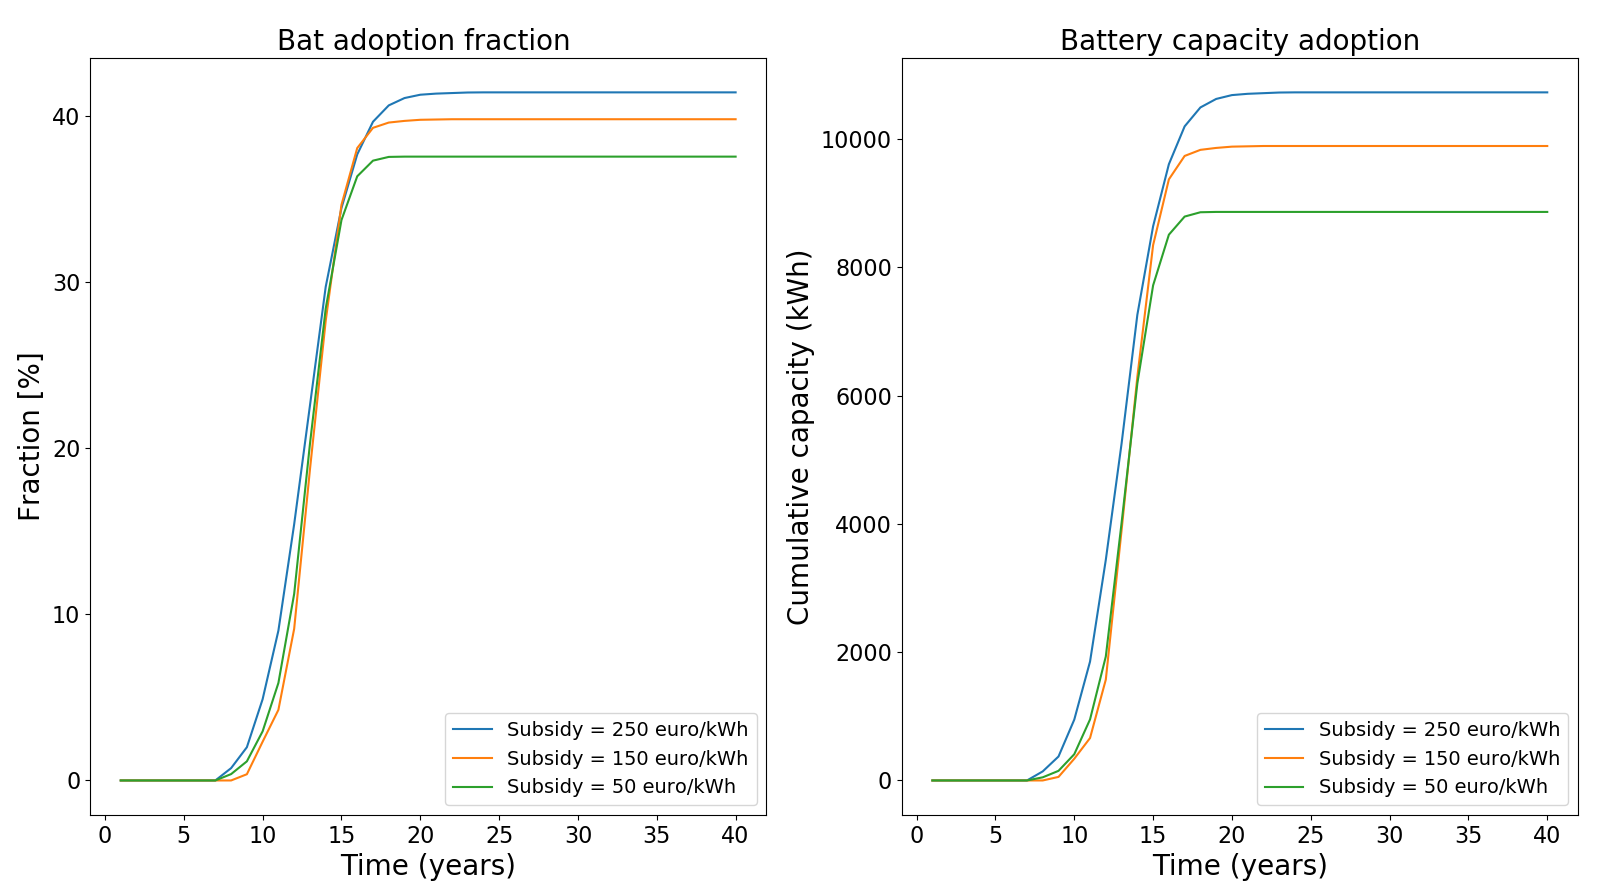
\includegraphics[width=12cm]{ModelAnalysis/Batsubs.png}
\caption{Battery adoption for different subsidies}
\label{Figure:batsubsvol}
\end{figure}
 \noindent
Contrary to the PV results, the battery subsidies show a very clear effect on the battery adoption data, as can be found in Figure \ref{Figure:batsubsvol}. The higher subsidies, the higher the adoption fraction and adopted capacity. The number of adopters for the \EUR{} 150 subsidy is 4.4\% lower than the case while being 9.9\% lower for the \EUR{} 50 subsidy. For the 150 \EUR{} option, the adopted capacity will be 7.5\% lower than in the base case, while for the 50 \EUR{} option, the adopted capacity will be 18.6\% lower than the base case. Both the adoption fraction and the adopted capacity are, therefore, increasing with an increasing subsidy. As can be seen from Figure \ref{Figure:configsubsvol}, one main trend will shape this adoption. 
\begin{figure}[h!]
\centering
\includegraphics[width=12cm]{ModelAnalysis/Configsubs.png}
\caption{Configurations for different subsidies}
\label{Figure:configsubsvol}
\end{figure}
 \noindent
 The higher the subsidies, the more the adoption will focus on the \textit{4kW/5kWh} configuration. 
Since this configuration will experience the effect of the subsidies fivefold (since a \textit{5kWh} battery is installed), this technology will become disproportionately popular (note how the 4\textit{kW}/2\textit{kWh} adopters even decrease for higher subsidies). The other configurations will be less popular since the subsidy effects are less present. In parallel with the adoption levels, the distribution tariff evolves to higher levels for the lowest subsidies, since the PV adoption levels are the highest for this specific policy. For the higher subsidies, the PV adoption is higher, causing the utility death spiral to manifest itself to a fuller extent.  
\begin{figure}[h!]
\centering
\includegraphics[width=6cm]{ModelAnalysis/Distsubs.png}
\caption{Distribution cost for different subsidies}
\label{Figure:distsubvol}
\end{figure}
 \noindent
Higher battery subsidies will, therefore, cause the adoption of the largest PV/battery systems to be encouraged. Lower subsidies can still encourage higher battery adoption without causing the adoption to be focused on one single configuration.
%\subsection{Network charge}
%\label{distanal} As was already discussed in Section \ref{compar}, the different network charges have a different effect on the savings and, therefore, the overall adoption and subsequent utility death spiral. The main driver for this difference in adoption between the net volumetric tariff and annual capacity offtake tariff is the difference in savings between the two tariffs. Both the way in which savings are created as well as the effect of this change in savings on the adoption of DER will be discussed in the next few paragraphs.
%\newline \newline \noindent
%Since the savings for a household due to the adoption of DER consist of both energy costs and (some) distribution costs, the overall savings will evolve with these components. In the case of the net volumetric distribution tariff, the distribution component can be calculated using Equation \ref{distnet}. This cost formula suggest that the savings of the household can increase substantially in case $q_{net}$ reaches a value close to zero. As can be seen in Figure \ref{Figure:netdem}, $q_{net}$  of all but two configurations is equal to zero, meaning that all distribution charges are avoided. Compared to $q_{net}$ for no DER adoption, the savings of the distribution component and by extension the electricity cost are significant. 
%\begin{figure}[h!]
%\centering
%\includegraphics[width=12cm]{ModelAnalysis/Netdemand.%png}
%\caption{Net volumetric demand for different DERs %configurations}
%\label{Figure:netdem}
%\end{figure}
%\noindent
%For the annual capacity offtake tariff, the distribution cost can computed using Equation \ref{qcap}. This network charge formulation suggests that, like in the volumetric case, the distribution cost could decrease to zero. When looking at Figure \ref{Figure:peakdem}, however, it becomes clear that $q_{cap}$ and the distribution cost component will remain strictly positive for all configurations.  
%\begin{figure}[h!]
%\centering
%\includegraphics[width=12cm]{ModelAnalysis/PeakDemand.png}
%\caption{Different peak demands}
%\label{Figure:peakdem}
%\end{figure}
%\noindent
%Due to the previously discussed difference in distribution cost for the two different network charges, the savings will de different, as can be seen in Figure \ref{Figure:Savings} \footnote{The represented data is the average of the savings for all configurations}. Here, it can be seen how the savings realised in the case of the net volumetric distribution tariff are much higher than for the annual capacity offtake tariff. Besides having a larger initial value, the savings for the volumetric network charge also increase more streadily than those in the capacity tariff case: the volumetric savings increase by 39.6\% throughout 40 year simulation, whereas they only increase by 6.8\% in the capacity case pver the same period. This is a direct result of the higher initial value in the volumetric distribution tariff case: the higher savings cause a higher adoption incentive, causing the utility death spiral to manifest itself more clearly, which will cause the distribution tariff to increase further. The results discussed in Section \ref{compar} showed the extent of this utility death spiral for the different policies. 
%\begin{figure}[h!]
%\centering
%\includegraphics[width=12cm]{ModelAnalysis/Savings.png}
%\caption{Savings for the volumetric and capacity tariff}
%\label{Figure:Savings}
%\end{figure}
\subsection{Preliminary analysis \& Conclusion}
Given the analysis of different parameters in the model, several conclusions can be drawn on a preliminary basis. First and foremost, the sensitivity analysis of the loss aversion showed how the adoption data can vary. A lower loss aversion causes the adoption to kick off sooner, while a higher loss aversion will have the opposite effect. Given the consistency of these results, further research into CPT as a decision-making theory in the DER adoption process could add valuable insights. 
%What also became clear from this analysis, is the role of the residual load in the DER adoption process. Since a lower residual load causes the network charges and savings to be higher, the incentive to adopt DER becomes higher, thereby reinforcing the network charge increase once again, creating a vicious circle. Currently, the fraction of DER in the overall electricity landscape still is limited, but rising quickly. Over the next few decades, as policy makers intend to make a large portion of the households adopt DER to reduce emissions, the residual load will become a smaller portion of the overall load, which would cause the utility death spiral effects to be amplified. The distribution cost evolution for low residual loads that was presented in Figure \ref{Figure:distresid} could, therefore, materialize over the next few decades if appropriate action is not taken. As was discussed in Section \ref{compar}, the capacity-based network charge can mitigate these effects. The main reason for this, as was discussed in Section \ref{distanal}, is the change in the distribution cost component and its effects on the savings and adoption incentive. For the net volumetric distribution tariff, this cost component decreases to zero for most configurations, generating more savings to the households and encouraging DER adoption. The design of the capacity offtake tariff, however, will cause the distribution component to decrease by a smaller amount for most configurations, generating less savings to the households, thereby encouraging DER adoption to a lesser extent. 
\newline \newline \noindent
Battery subsidies can help enhancing the adoption of batteries. Higher subsidies result in a higher cumulative PV capacity, higher battery adoption fraction and significantly higher cumulative battery capacity. The main driver for this increase in adoption and capacity is the increased popularity of the 4\textit{kW}/5\textit{kWh} configuration. It is, therefore, questionable if the battery subsidy should be that high, since this configuration will cause a lot of grid injection and grid stability issues. More fundamentally, though, the question is whether battery subsidies are necessary altogether. Since the battery adoption fraction increases from 37.3\% to 41.4\% for the lowest to the highest subsidy (see Figure \ref{Figure:batsubsvol}), the efficiency of these subsidies is questionable. Since the cumulative capacity increases from about 8,600 to 10,600 \textit{kWh}, the subsidies increase from \EUR{} 430,000 to \EUR{} 2,650,000. This 516\% increase in subsidies for a 23.2\% increase in battery capacity and an 11\% increase in adoption seems like a waste of government resources. These subsidies are to be monitored closely and reduced significantly once battery costs decrease and the adoption rates start increasing, since a continuation of these subsidies could be financially wasteful. 
\newline \newline \noindent
Next to the insights gathered in this section, the analysis of different parameters embedded in the model also gives rise so several points of attention. The most important one also relates to the loss aversion. In this Thesis, the used value is the one that based on the measurements performed by Bougherare et al. \cite{lossaversions}, which was set at $\lambda = 1.5$. However, since this value is the result of experimental data, just like the values measured by Kahneman and Tversky, the transposition of the loss and risk aversion value to this Thesis is an assumption that is to be validated by performing field experiments with energy prosumers being the target. As the sensitivity analysis showed, a variation of the loss aversion causes the results to vary significantly. An incorrect estimate of the loss aversion could, therefore, cause the results to deviate significantly. 
\newline \newline \noindent
In addition, the analysis of the battery subsidies was done under the current projections for cost decrease. Since battery technology currently is in a period of rapid growth, the development of this DER can follow many different paths. A sudden change in technology or policies could, therefore, discredit the results discussed in this Thesis. In addition, the combination of constant subsidies throughout the simulation combined with the cost reduction of the battery technology could give a rather optimistic view on the battery adoption.
\newline \newline \noindent
Note that this list of parameters susceptible to a sensitivity analysis is not comprehensive. Note that one important parameter that needs further analysis in this context is the time value of money or discount factor $r$. As was discussed in Section \ref{Investmentss}, many of the characteristics of investments in DER are a function of time, like long-run uncertainties, long payback periods and investment postponement options. This makes the time preference of the investor important in the adoption process. In future work, therefore, different time preference and loss aversion configurations should be tested. 
\section{Comparison to EUT} \label{EUTcompar}
Since this Thesis uses CPT for the simulation of investments in DERs, a comparison to the most common decision-making theory, the EUT, can provide additional insights into the model. By comparing these two decision-making theories, the potential benefits or drawbacks of CPT over EUT can be discussed. This will be done for both the annual net metering and annual capacity offtake tariff. The other policies can be found in Appendix \ref{app:3}. 
\newline \newline \noindent
The decision variable for the EUT is the overall payback period of the different configurations (since this theory does not take into account a reference point of the current situation/level as CPT does). The utility of the payback period will be normalised according to the method proposed by Zhao et al. \cite{ABMPV}:
\begin{equation} \label{EUTnorms}
	NUT_{eco,i} = \frac{Max(UT) - UT_{i}}{Max(UT) - Min(UT)}
\end{equation}
Besides this difference, the implementation of the EUT in the ABM is identical to that of the CPT to guarantee both simulations are as comparable as possible. The analysis is, therefore, done on a "ceteris paribus" basis. In the following sections, the comparison of CPT with EUT will be done in the net metering case for both tariff structures.
\subsection{Annual net metering}
For the annual net metering policy, the PV adoption using EUT can be found in Figure \ref{Figure:PVeut}. This adoption shows an S-shaped adoption pattern, much like the CPT results do, except for the beginning of the adoption process. This shows that the adoption using EUT follows the sequence of innovators, early adopters all the way down to laggards, which corresponds to Rogers' theory of innovation and the results sequence of the CPT. Note that the final adoption fraction in the case of the EUT also is 50\%, meaning that all household that could have adopted DER have done so. Where the EUT simulation shows some significant differences with the CPT, as can be seen in Figure \ref{Figure:PVcompar}, is in the rate of adoption. 
%\begin{figure}[h!]
%\centering
%\includegraphics[width=12cm]{EUTCompar/PVEUT.png}
%\caption{PV adoption under EUT}
%\label{Figure:PVeut}
%\end{figure}
 %\noindent 
 Under CPT, the adoption is a gradual process where the technologies get adopted over a period of about 10 years. The adoption will also kick off in year 6-7, since the adoption threshold is only reached in this period. The EUT results, however, show an adoption process starting in year 1, followed by a very rapid adoption process to full adoption. Comparing the two simulations with each other, CPT does seem to create a more realistic simulation of the PV adoption process. Note that the adoption fraction is 50\% (i.e. full adoption) for both decision making theories, but the overall adopted capacity is higher for the CPT. This is mainly because the EUT simulation tends to focus the adoption on cheap/small configurations with a low capacity, which will be discussed in the next paragraphs.
\begin{figure}[h!]
\centering
\includegraphics[width=12cm]{EUTCompar/PV.png}
\caption{PV adoption comparison}
\label{Figure:PVcompar}
\end{figure}
%\newline \newline
\noindent
Whereas the PV adoption shows an S-shaped adoption curve, this does not apply to the battery technology. The battery adoption results for the EUT remain equal to zero, as can be seen in Figure \ref{Figure:bateut}. A comparison of this adoption data with the data of the CPT can be found in \ref{Figure:batcompar}:
%\newline
%\begin{figure}[h!]
%\centering
%\includegraphics[width=12cm]{EUTCompar/BatEUT.png}
%\caption{Battery adoption under EUT}
%\label{Figure:bateut}
%\end{figure}
%\noindent
%\newline
\begin{figure}[h!]
\centering
\includegraphics[width=12cm]{EUTCompar/Bat.png}
\caption{Battery adoption comparison}
\label{Figure:batcompar}
\end{figure}
%\newline 
\noindent
The main reason for this lack of battery adoption is because the adoption will happen according to the normalised payback period. The higher the payback period, the lower the normalised utility is, according to Equation \ref{EUTnorms}. The preferred options, therefore, will be those with the lowest overall payback. As can be seen from Figure \ref{Figure:payback}, the 1.5 \textit{kW} and 2.5 \textit{kW} configurations without any batteries have the lowest payback period. These technologies will, therefore, have the highest economic utility and will be the preferred options for the households. As a result, no batteries will be adopted under the EUT simulation. In fact, the EUT model would require battery subsidies that exceed the capital cost of the battery technology to encourage any adoption of battery configurations.
\newline 
\begin{figure}[h!]
\centering
\includegraphics[width=12cm]{EUTCompar/Payback.png}
\caption{Initial payback periods}
\label{Figure:payback}
\end{figure}
\newline \newline \noindent
This shows how the EUT is less refined and complex as a decision-making theory, since there is a subtle bias in the selection. Due to the reference level incorporated in the CPT, different households have different utility patterns which will cause the adoption to be more diverse: laggards can have a completely different economic view on a certain configuration than innovators do. The added level of complexity that CPT modeling requires by incorporating loss aversion and reference levels, controversial though these concepts may be, seem to show their added value in the results, since results using this theory are less lopsided than the EUT results. 
\newline \newline \noindent
When looking at how the overall configuration distribution compares for both decision making theories, there is a very clear difference in the results, as can be seen in Figure \ref{Figure:configeut}. This data reconfirms the aforementioned bias of EUT towards small PV configurations without batteries: the overwhelming majority of configurations adopted under EUT is the 1.5\textit{kW} PV installation, with a small minority in 2.5\textit{kW} configurations adopted. When using the CPT, the adoption is more granular between the different technologies, both standalone PVs and PV-battery systems, with 4\textit{kW}/2\textit{kWh} and 4\textit{kW}/5\textit{kWh} being the most popular.
\begin{figure}[h!]
\centering
\includegraphics[width=12cm]{EUTCompar/Config.png}
\caption{Configurations comparison}
\label{Figure:configeut}
\end{figure}
\noindent
In parallel with the adoption for the different decision making theories, the network charge will evolve to very rapidly for the EUT and at a slower but more steady rate for the CPT.
\begin{figure}[h!]
\centering
\includegraphics[width=10cm]{EUTCompar/Dist.png}
\caption{Distribution cost comparison}
\label{Figure:distcompar}
\end{figure}
\subsection{Annual capacity offtake tariff}
The PV adoption for the annual capacity offtake tariff can be found in Figure \ref{Figure:PVeutcap}. Here, the adoption trend of the PV technology can be seen, which starts quickly in the beginning (innovators and early adopters), followed by a period of rapid adoption, only to end with a period of saturated adoption (when the laggards will adopt). The adoption does, therefore, once again follow and S-shaped evolution, except for the start of the adoption. 
\newline
\begin{figure}[h!]
\centering
\includegraphics[width=14cm]{EUTCompar/PVEUTcap.png}
\caption{PV adoption under EUT}
\label{Figure:PVeutcap}
\end{figure}
\noindent 
When comparing the results of the EUT with those of the CPT, as can be seen in Figure \ref{Figure:PVcomparcap}, there is a big difference in the adoption trend. As was the case for the net volumetric distribution tariff, the adoption in the EUT case will happen both earlier in the simulation and more quickly, whereas the adoption in the case of the CPT will both happen in a later stage and happen at a slower but steadier rate. Despite both decision making theories providing results that correspond to the logic behind Rogers' adoption process of innovation diffusion, the scale of this adoption process is rather different. Both simulations start with lower adoption rates, followed by higher adoption rates only to saturate toward the final adoption rate. In the case of the EUT, however, this adoption process happens very sudden, whereas the process is much more gradual for the CPT simulation. As was the case with the net volumetric distribution tariff, these results both confirm the validity of the separate decision making theories with regards to the adoption process, but the vast difference in the overall adoption process gives rise to one major question, which is why the adoption process is so different for the two decision making theories.
 \newline \noindent
 \begin{figure}[h!]
\centering
\includegraphics[width=14cm]{EUTCompar/Pvcap.png}
\caption{PV adoption comparison}
\label{Figure:PVcomparcap}
\end{figure}
\newline \newline \noindent
One of the main reasons, for this difference in adoption, as was the case with the net volumetric distribution tariff, is the incorporation of loss aversion into the simulation by using CPT. According to Equation \ref{EUTnorms}, the normalised economic utility of the configurations cannot be negative. This implies that however large the payback period of the different configurations, there will still be some level of positive economic utility to the investment options under consideration. This will implicitly make the household more prone to adopt one of the DERs available. When using the CPT, on the other hand, there will be a clear distinction between configurations that the household will consider as being economically attractive and those that he considers economically disadvantageous. Given the fact that the loss aversion will make the households "overweight" the negative prospects of those disadvantageous configurations by a factor of 2.25, households will be loss prone to adopt one of the DERs at hand. Since the households will initially be a bit "frightened" by the negative prospects of the DERs, adoption will only happen in a later stage, when cost reduction effects have manifested themselves sufficiently to make the overall prospects more positive. 
\newline \newline \noindent
The battery adoption for the capacity tariff under EUT can be found in Figure \ref{Figure:bateutcap}.
\newline
\begin{figure}[h!]
\centering
\includegraphics[width=14cm]{EUTCompar/BatEUTCap}
\caption{Battery adoption under EUT}
\label{Figure:bateutcap}
\end{figure}
\newline
\noindent 
Contrary to the net volumetric distribution tariff case, the EUT simulation under the annual capacity offtake tariff will result in battery adoption. This adoption process also saturates to a level of full adoption. The adoption process will also follow the known S-curved adoption process, except for the start of the adoption where the adoption rate is higher. When comparing this data to the CPT case, as can be seen in Figure \ref{Figure:batcomparcap}, the adoption data once again shows a big difference for the two different decision making theories. As was the case for PV adoption, the battery adoption using the EUT happens at an earlier stage and at quicker rates.
\begin{figure}[h!]
\centering
\includegraphics[width=14cm]{EUTCompar/BatCap.png}
\caption{Battery adoption comparison}
\label{Figure:batcomparcap}
\end{figure}
\noindent 
Once again, this is due to the popularity of certain configurations. Figure \ref{Figure:paycap} show how the 2.5\textit{kW}/2\textit{kWh} and 4\textit{kW}/2\textit{kWh} configuration have the lowest payback period in the EUT simulation for the annual capacity offtake tariff. This is due a combined effect of the low peak capacity (see Section \ref{distanal}) and the initial investment cost. Although the peak capacity of the 4\textit{kW}/5\textit{kWh} configuration is the lowest of all the options (see Figure \ref{Figure:peakdem}), the savings due to this lower peak capacity are not sufficient to compensate for the higher investment cost. 
\newline 
\begin{figure}[h!]
\centering
\includegraphics[width=10cm]{EUTCompar/PayCap.png}
\caption{Initial payback periods}
\label{Figure:paycap}
\end{figure}
 \newline \newline \noindent 
 This combined effect of savings and investment cost will make the 4\textit{kW}/2\textit{kWh} configuration the most popular, as can be seen in Figure \ref{Figure:comparcap}. Whereas the CPT simulation shows a distribution of the different configurations adopted, the EUT simulations shows a very clear adoption bias towards the two aforementioned configuration. 
 \begin{figure}[h!]
\centering
\includegraphics[width=10cm]{EUTCompar/ConfigCap.png}
\caption{Configurations comparison}
\label{Figure:comparcap}
\end{figure}
\newline \newline \noindent 
 As a final note, the capacity offtake tariff evolution can be found in Figure \ref{Figure:captar}.  Given the further stage of DERs adoption in the case of EUT, the capacity tariff will decrease further, due to reasons explained in Section \ref{distanal}. 
\begin{figure}[h!]
\centering
\includegraphics[width=10cm]{EUTCompar/CapTar.png}
\caption{Capacity tariff evolution}
\label{Figure:captar}
\end{figure}
\subsection{Preliminary analysis \& Conclusion}
With the previously discussed data in mind, EUT does seem to present much cruder results than the CPT. The added complexity of accounting for loss aversion and the reference level of each decision maker (by comparing the expected payback period with the actual payback period of configurations) clearly adds an additional level of complexity to the results. Given the more gradual adoption of technologies due to the loss aversion and the more granular adoption of different technologies by accounting for the reference level of each household, this added level of complexity does appear to add relevance to the results. 
\newline \newline \noindent
Considering the fact that only two utility attributes (economic and social utility) were used in this simulation, whereas other works use three or more utility attributes \footnote{Zhao et al. \cite{ABMPV} consider payback periods, household income, advertisement and neighborhood effects as utility attributes in their model whereas Palmer at al. \cite{ItalyAdoption} consider the payback period, environmental benefits, household income and communication effects as attributes in their model}, elaborating on these utility attributes using CPT could generate results of increased quality and resemblance to real-life adoption data. 
\newline \newline \noindent
Despite the fact that many items still need addressing in this setting, like a further diversification of the economic factors in the model, the constant weighting coefficients in the utility and the extent of the utility attributes themselves, the presented results have made a strong case for CPT as a decision making theory in the simulation of investments in DERs in consumer-centric energy systems.
\section{Discussion \& Future work} \label{future}
In this section, the results of the model were discussed in order to address the research question and the complementary sub-questions. This discussion was separated according to these research questions. The first research question related to the evaluation of different policies with regards to the DER adoption and utility death spiral. The main takeaways here are:
\begin{itemize}
\item The net billing policy can serve as an efficient way to encourage rapid adoption of small-scale DERs. These installations will predominantly serve the inflexible demand of the households and inject a limited amount of electricity into the grid.
\item The net metering policy and additional battery subsidies can serve as a way to encourage large cumulative adoption capacity of DERs installations. These policies will, however, cause larger amounts of grid injection. Their efficiency is, therefore, questionable.
\item The net volumetric distribution tariff will encourage larger and quicker adoption of PV and batteries due to larger savings. In parallel, the utility death spiral (i.e. tariff modification by the DSO) will manifest itself more clearly. The capacity offtake tariff, on the other hand, can partially mitigate the effects on this utility death spiral, indicating that this network charge is preferable in the future grid, where widespread DER adoption and the subsequent utility death spiral are extremely likely prospects. 
\end{itemize}
The second Research Question, which is a sub-question to the main Research Question, relates to the sensitivity of certain parameters embedded in the model. 
\begin{itemize}
\item The selected value for the loss aversion coefficient ($\lambda = 1.5$)  can provide a consistent set of results and suggest that future research into adequate values of this parameter can add valuable insights. 
\item The lower the residual load the DSO can rely on, the more the utility death spiral will manifest itself. In the future grid, where DER adoption becomes more pervasive, this effect will become increasingly present and is a threat that must be anticipated. The capacity tariff is a means to mitigate this utility death spiral effect.
\item Battery subsidies can help encouraging the adoption of residential batteries combined with PV, but the main effect of these subsidies is the increased adoption of the largest configurations available, causing large-scale grid injection. Given the amount of government resources these subsidy programs require, this subsidy may not be necessary if the battery technology sufficiently expands and scales in cost in the near future, since the battery cost reduction also is an important driver in the battery adoption process. 
\end{itemize}
The third Research Question, which also is a sub-question to the main Research Question, relates to the comparison of the model results with the EUT.
\begin{itemize}
\item  CPT as a decision making theory to simulate the adoption of DER in consumer-centric energy systems can complement the results provided by the EUT.
\item The results of EUT compared to the CPT are cruder and less refined, since the adoption does not follow the same adoption trend and tends to focus the adoption or one of two configurations. 
\item Despite uncertainty concerning some of the parameters in CPT, like the loss aversion, risk aversion and reference levels, this theory can capture more complex behavior of decision makers, like being able to describe a more diverse configuration adoption.
\end{itemize}
\newline \newline \noindent
Despite these insights, further work still needs to be done in this field. First and foremost, since this Thesis attempted to provide qualitative insights into this novel approach to the simulation of DER adoption by using CPT, a case test must be performed to relate this research to the real world. This must be complemented by field experiments where energy prosumers are the targets to be able to measure an accurate value of the loss aversion, risk aversion and reference levels. In addition, a number of items need further elaboration:
\begin{itemize}
\item Since the utility calculation only considers economic and social utility but many more factor have an effect on the adoption such as advertisements, household profiles etc, the utility attributes must be extended beyond the two considered in this Thesis.
\item Some implicit assumption made concerning the behavior of the households, like the absence of the rebound effect and the indifference of the residual households towards the increase in distribution tariffs, must be elaborated upon. 
\item Since the diversification of the household was limited to the financial wealth of the household, this diversification must be elaborated to social, geographical and cultural factors influencing the nature of the households and his position towards DERs adoption under uncertainty.
\item The assumption of constant weighting coefficients and the constant adoption nature of the different households must be elaborated to a model where these parameters also become endogenous to the model and change over time: initially the economic weighting coefficient should be larger, but as the adoption proceeds over time, the social weighting coefficient should be larger.
\item Whereas this Thesis considers the different policies separately, different combinations the presented policies should be examined to find an optimal structure that can combine the positive effects of the respective policies while minimizing the negative effects of these programs. An example could be a policy that combines the quick adoption rates of the net billing policy with the limited utility death spiral effects of the annual capacity offtake policy. 
\item In addition to the parameters tested in the model, the time preference behavior of the households, which is captured through the discount factor, must be included in the model analysis. In doing so, this must be related to the loss aversion of the households to test different configurations of this behavior. 
\end{itemize}
Despite these items that need further work in this field, the results in this chapter have made a strong case for further research into CPT in an ABM for the simulation of DER adoption in a consumer-centric energy system, which was assumed to be a CAS. 
    
\chapter{Conclusion}
In the wake of recent trends in the electricity markets like liberalisation and emission reduction, DER like solar PV and residential batteries are experiencing periods of rapid growth and cost reduction. To further enhance the adoption of these technologies, governments have put up incentive programs to encourage households to adopt renewable energy technologies in a residential setting. These include annual net metering, annual capacity offtake, net billing and battery subsidies. The effects of these incentives on the households' behavior are, however, a major point of ongoing research. This is mainly because the simulation of households' behavior requires the arduous task of incorporating human factors like loss aversion and irrational decision making. This Thesis bridges the gap between the ongoing research in DER adoption modeling, which mainly uses EUT, and the novel concept in behavioral economics that is cumulative prospect theory (CPT).
These concepts from behavioral economics will be combined with an agent-based modeling (ABM) framework to simulate the behavior of the system, which is assumed to be a complex adaptive system (CAS). To that end, this Thesis attempts to perform a more accurate simulation of the behavior of households in the DER adoption process. By examining the DER adoption and distribution tariff data for the different policies, insights about the effectiveness of the different policies can be provided. With these insights, policy makers can identify what policies they want to put in place as a function of their priorities with regards to energy policy. 
\newline \newline \noindent
An optimization model was developed to determine the optimal costs and revenues of different PV/battery configurations. These results were be interpreted by a model that incorporates the behavioral factors of CPT like loss aversion and the reference situation of the households. According to these results, households adopted certain configurations. This adoption causes the aggregate energy demand to decrease, putting the revenue of the DSO at risk. This will force the DSO to increase the network charge, causing the savings for the household to increase, creating a vicious circle of increasing savings and adoption. This model was tested for four cases: (i) annual net metering, (ii) annual capacity offtake, (iii) net billing and (iv) battery subsidies. In this setting, the main Research Question and two sub-questions were answered.
\newline \newline  \noindent
\textbf{Research question 1: What is the effect of annual net metering, annual offtake capacity tariff, net billing, feed-in tariffs, and subsidies on both households' DERs adoption under uncertainty and the utility death spiral?}
\newline \newline \noindent
As became clear from the results discussion, different policies have different benefits. If the policy put in place by the government intends to encourage the rapid adoption of small-scale DER that mainly serve the households' residential demand without injecting vast amounts of electricity into the grid, the net billing policy is a good candidate. This policy will cause the adoption to kick off earlier and happen more quickly. The overall adopted capacity, however, will be rather low. This has both benefits as well as drawbacks. Since the adoption by households in the net billing case happens mainly with the intention of supplying the residential demand without injecting vast amounts of excess electricity into the grid, net billing will cause less stresses onto the grid. Since the frequency and voltage stability issues due to grid injection by intermittent RES are also a major concern in the energy transition, net billing can serve as an effective policy to avoid these grid stability issues indirectly. The overall adopted capacity and produced energy by the DER will, however, be lower in the case of the net billing policy. The overall RES penetration will, therefore, be lower. 
\newline \newline \noindent 
If the policy makers intend to maximize the cumulative adopted capacity of RES, both in PV and battery technology, the net metering policy is more suitable. Since this policy incentivizes households to adopt larger installations, the overall capacity will be visibly larger. This will, however, cause the grid injection to be larger. The grid stability could, therefore, deteriorate under a net metering policy. If policy makers anticipate this and intend to encourage widespread injection into the grid, which is unlikely, net metering is the appropriate policy. 
\newline \newline \noindent
If policy makers want to increase the rate of battery adoption, battery subsidies can be introduced. Although this will not cause the adopted battery capacity to increase exponentially, this incentive can have a visible effect on the batteries, since this technology has not yet had the same adoption and popularity as PV, causing the costs to remain high. The analysis in this Thesis showed that the battery subsidies do not need to be extremely large and that the effect of increasing the subsidies will have a saturating effect on the battery adoption. To limit waste of government resources, therefore, these subsidy programs must be closely monitored. 
\newline \newline \noindent
In addition to the main Research Question of this Thesis, two complementary sub-questions were also part of this research. 
\newline \newline \noindent
\textbf{Research sub-question 1: What is the effect of risk aversion, peer influence and network charges on both the DERs adoption on a household level and the utility death spiral?}
\newline \newline \noindent
For all these policies, the utility death spiral will manifest itself. The annual capacity offtake policy, however, will limit the extent of the utility death spiral. Due to lower savings for the households, however, this policy will cause slower adoption.  Depending on the residual load, the extent of the utility death spiral will vary: the lower the residual load, the less reserve revenue the DSO can rely on and the more the distribution tariff will have to be adapted. Consequently, the lower residual load will cause the DER adoption to happen more quickly. The analysis that has been performed in this Thesis, therefore, was able to show how the DSO should beware of this effect for the volumetric distribution tariff. A possible solution to this problem, as was also analysed in this Thesis, is the introduction of the annual capacity offtake tariff. Due to the different approach of this tariff structure (i.e. as a function of the peak capacity instead of the electricity consumption), the tariff will have to be changed to a lesser extent for DER adoption. Since the tariff will increase less quickly, the savings will be be lower than in the volumetric tariff case. This will cause the subsequent DER adoption to be lower. 
\newline \newline \noindent
\textbf{Research sub-question 2: What is the added value of using a cumulative prospect theory to model investment decision making, compared to expected utility theory?}
\newline \newline \noindent
With regards to the implementation of CPT into this model, the loss aversion sensitivity analysis that was discussed clearly showed how the loss aversion variation causes the adoption to be delayed or occur earlier. This analysis showed the consistency of the results, making a case for further research into this decision-making theory for the simulation of DER adoption. Compared to the EUT results, the added complexity and uncertainty concerning CPT parameters like loss aversion and reference levels also showed to pay off, since the adoption data of the EUT showed much cruder patterns.
\newline \newline \noindent
In future work, the utility attributes can be extended beyond the economical and social one that were considered in this Thesis. Since earlier work (using the EUT) considered additional factors like advertisement effects and household income effects, these can be integrated into the developed model to further refine the model and capture additional behavioral factors. This item has two sub-items that also need further addressing in future work.
\newline \newline \noindent
First of all, since the utility was calculated as a weighted average of social and economical utility using constant coefficients, these coefficients were treated as exogenous variables. In reality, however, these coefficients will change over time, since economical considerations no longer prevail once widespread adoption has been reached, which was assumed in this model. By capturing this shift in weighting coefficients, the model will become even more representative of the adoption process. 
\newline \newline
Secondly, the economic assumptions with regards to the household can be further elaborated upon. Since the model in this Thesis only considers the financial wealth of the households as a proxy for the variation in residential electricity demand, many additional factors can be considered, such as the household size, household age etc. An elaboration of the economic characteristics of the agents in the model could, therefore, also refine the model even further. 
\newline \newline \noindent
In addition, with the knowledge gathered in this Thesis concerning the different policies, these policies can be combined to determine the optimal combination of these different programs in order to maximize the benefits of the different programs, like combining the adoption speed of the net billing policy with the limited utility death spiral of the annual capacity offtake. In doing so, the negative effects of these respective policies must be minimized with regards to all actors in the DER fueled grid transformation process. Furthermore, the sensitivity analysis must be elaborated to more parameters, most notably the time preference of the decision maker. 
\newline \newline \noindent
As a final point of further work, the qualitative study of this model must be extended to a case study taking into account the insights provided in this model. This will allow for the model to be set up under the correct assumptions to simulate the behavior in a real world case. To measure accurate values of the CPT parameters, a field experiment where energy prosumers are the target could also add significant value to this field of research. 





    

% Indien er bijlagen zijn:
\appendixpage*          % indien gewenst
\appendix
%\chapter{Household optimization model}
\label{app:A}
The optimization model discussed in section \ref{submodel} describes how the savings of a household PV-battery configuration can be calculated. To provide some insights into the underlying results of this submodel, an overview of some results will be presented to show the validity of the results the model gives.
\newline \newline \noindent
The main variables of the optimization problem are the net demand $q[t]$, battery charging $ch[t]$, battery discharging $dch[t]$ and battery energy level $e_{BAT}[t]$. The charging and discharging power for a $4kW_p - 5kWh$ battery configuration can be found in figure \ref{figure:charge}.
\newline 
\begin{figure}[h!]
\centering
\includegraphics[width=8cm]{(Dis)charge.png}
\caption{Charging and discharging profile of the residential battery}
\label{figure:charge}
\end{figure}
\newline 
The associated energy levels of the battery can be found in figure 
\newline 
\begin{figure}[h!]
\centering
\includegraphics[width=12cm]{energy.png}
\caption{Energy levels battery}
\label{figure:charge}
\end{figure}
\newline
%%% Local Variables: 
%%% mode: latex
%%% TeX-master: "thesis"
%%% End: 

\chapter{Sensitivity analysis other policies}
\label{app:2}
In this Appendix, the sensitivity analysis of the parameters discussed in Section \ref{analysis} will be presented for the remaining policies: battery subsidies, net billing and the annual offtake capacity tariff. 
\section{Residual load}
\subsection{Battery subsidies}
The data for the residual load sensitivity analysis of the battery subsidy policy (combined with the net metering policy) can be found in Figures \ref{fig:M}, \ref{fig:N}, \ref{fig:O} and \ref{fig:P}. 
\newline 
\begin{figure}[h!]
    \centering
    \includegraphics[width=10cm]{AppendixA/PVSubsresid.PNG}
    \caption{PV adoption for different residual loads}
    \label{fig:M}
\end{figure}
\noindent
\newline 
\begin{figure}[h!]
    \centering
    \includegraphics[width=10cm]{AppendixA/BatSubsresid.PNG}
    \caption{Battery adoption for different residual loads}
    \label{fig:N}
\end{figure}
\noindent
\newline 
\begin{figure}[h!]
    \centering
    \includegraphics[width=10cm]{AppendixA/ConfigSubsresid.PNG}
    \caption{Configurations for different residual loads}
    \label{fig:O}
\end{figure}
\noindent
\newline
\begin{figure}[h!]
    \centering
    \includegraphics[width=10cm]{AppendixA/DistSubsresid.PNG}
    \caption{Normalised capacity tariff for different residual loads}
    \label{fig:P}
\end{figure}
\subsection{Net billing}
The data for the residual load sensitivity analysis of the net billing policy can be found in Figures \ref{fig:R}, \ref{fig:S}, \ref{fig:T} and \ref{fig:U}. 
\newline 
\begin{figure}[h!]
    \centering
    \includegraphics[width=10cm]{AppendixA/PVNBresid.PNG}
    \caption{PV adoption for different residual loads}
    \label{fig:Q}
\end{figure}
\noindent
\newline 
\begin{figure}[h!]
    \centering
    \includegraphics[width=10cm]{AppendixA/BatNBresid.PNG}
    \caption{Battery adoption for different residual loads}
    \label{fig:R}
\end{figure}
\noindent
\newline 
\begin{figure}[h!]
    \centering
    \includegraphics[width=10cm]{AppendixA/ConfigNBresid.PNG}
    \caption{Configurations for different residual loads}
    \label{fig:S}
\end{figure}
\noindent
\newline
\begin{figure}[h!]
    \centering
    \includegraphics[width=10cm]{AppendixA/DistNBresid.PNG}
    \caption{Normalised capacity tariff for different residual loads}
    \label{fig:T}
\end{figure}%
\subsection{Annual capacity offtake}
The data for the residual load sensitivity analysis of the annual capacity offtake 
\newline 
\begin{figure}[h!]
    \centering
    \includegraphics[width=10cm]{AppendixA/PVCapresid.PNG}
    \caption{PV adoption for different residual loads}
    \label{fig:U}
\end{figure}
\noindent
\newline 
\begin{figure}[h!]
    \centering
    \includegraphics[width=10cm]{AppendixA/BatCapresid.PNG}
    \caption{Battery adoption for different residual load}
    \label{fig:V}
\end{figure}
\noindent
\newline 
\begin{figure}[h!]
    \centering
    \includegraphics[width=10cm]{AppendixA/ConfigCapresid.PNG}
    \caption{Configurations for different residual loads}
    \label{fig:W}
\end{figure}
\noindent
\newline
\begin{figure}[h!]
    \centering
    \includegraphics[width=10cm]{AppendixA/CapTarresid.PNG}
    \caption{Normalised distribution tariff for different residual loads}
    \label{fig:X}
\end{figure}

\chapter{EUT comparison}
\label{app:3}
\section{Net billing}
The data for the loss aversion sensitivity analysis of the battery subsidy policy (combined with the net metering policy). 
\newline 
\begin{figure}[h]
    \centering
    \includegraphics[width=12cm]{EUTAppendix/PVNB.PNG}
    \caption{PV adoption for CPT \& EUT}
\end{figure}
\noindent
\newline 
\begin{figure}[h]
    \centering
    \includegraphics[width=12cm]{EUTAppendix/BatNB.PNG}
    \caption{Battery adoption for CPT \& EUT}
\end{figure}
\noindent
\newline 
\begin{figure}[h]
    \centering
    \includegraphics[width=12cm]{EUTAppendix/ConfigNB.png}
    \caption{Configurations for CPT \& EUT}
\end{figure}
\noindent
\newline
\begin{figure}[h]
    \centering
    \includegraphics[width=12cm]{EUTAppendix/DistNB.png}
    \caption{Normalised distribution tariff for CPT \& EUT}
\end{figure}
\newpage}

\section{Battery subsidies}
The data for the loss aversion sensitivity analysis of the battery subsidy policy (combined with the net metering policy). 
\newline 
\begin{figure}[h]
    \centering
    \includegraphics[width=12cm]{EUTAppendix/PVSubs.png}
    \caption{PV adoption for CPT \& EUT}
    \label{fig:}
\end{figure}
\noindent
\newline 
\begin{figure}[h]
    \centering
    \includegraphics[width=12cm]{EUTAppendix/BatSubs.png}
    \caption{Battery adoption for CPT \& EUT}
    \label{fig:}
\end{figure}
\noindent
\newline 
\begin{figure}[h]
    \centering
    \includegraphics[width=12cm]{EUTAppendix/ConfigSubs.png}
    \caption{Configurations for CPT \& EUT}
    \label{fig:}
\end{figure}
\noindent
\newline
\begin{figure}[h]
    \centering
    \includegraphics[width=12cm]{EUTAppendix/DistSubs.png}
    \caption{Normalised distribution tariff for CPT \& EUT}
    \label{fig:}
\end{figure}
\newpage}


%%% Local Variables: 
%%% mode: latex
%%% TeX-master: "thesis"
%%% End: 

% ... en zo verder tot


\backmatter
% Na de bijlagen plaatst men nog de bibliografie.
% Je kan de  standaard "abbrv" bibliografiestijl vervangen door een andere.
\bibliographystyle{ieeetr}
\bibliography{references}
\end{document}

%%% Local Variables: 
%%% mode: latex
%%% TeX-master: t
%%% End: 
